\documentclass{report}
\usepackage[utf8]{inputenc}
\usepackage{graphicx}
\graphicspath{ {./images/} }
\usepackage{subfig}

\usepackage{algorithm}
\usepackage{algpseudocode}
\usepackage{pdfpages} 
\usepackage{xcolor}


\begin{document}

\includepdf[page={1}]{capa_dissertacao}
\newpage
\begin{abstract}
This thesis presents a comprehensive machine learning approach to model and predict the power output of photovoltaic (PV) panels. It investigates the influence of various factors on the performance of PV panels, including weather conditions and external influences. The study develops a machine learning model using the Python programming language and the scikit-learn library.\\
\\
The model is trained and evaluated on a carefully curated dataset of PV power output measurements. Rigorous performance metrics are employed to assess the accuracy and reliability of the model's predictions. The results demonstrate the effectiveness of the machine learning techniques in accurately forecasting the power output of PV systems.\\
\\
Furthermore, the project delves into the potential implications of government policies and incentives in facilitating the growth and development of the PV industry. It highlights the significant benefits of expanding the utilization of renewable solar energy sources. Detailed discussions on the role of supportive policies and incentives shed light on how the PV industry can thrive in the future.\\
\\
While achieving commendable results, this project acknowledges the need for continuous improvements and future research in the modeling and measurement of PV panels. Specific areas for future exploration include advanced feature engineering techniques, incorporation of real-time weather data, and the integration of additional data sources to enhance the accuracy and robustness of the models.\\
\\
In summary, this project showcases a machine learning-based approach to accurately predict the power output of PV panels. It underscores the importance of supportive government policies and incentives for the growth of the PV industry. The findings and future research directions presented in this study contribute to the advancement of renewable energy technologies and their sustainable integration into our energy systems.\\
\\
\textbf{Keywords:} Photovoltaic panels, Power output prediction, Machine learning, Weather conditions, External influences, Python programming, Scikit-learn library, Dataset, Performance metrics, Accuracy, Reliability, Government policies, Incentives, Renewable energy, Solar energy, Feature engineering, Real-time weather data, Data integration, Sustainable energy, Energy systems, Future research.
\end{abstract}\\

\section*{Resumo}
Esta tese apresenta uma abordagem abrangente de aprendizado de máquina para modelar e prever a saída de energia de painéis fotovoltaicos (PV). Investiga a influência de vários fatores no desempenho dos painéis PV, incluindo as condições climáticas e influências externas. O estudo desenvolve um modelo de aprendizado de máquina usando a linguagem de programação Python e a biblioteca scikit-learn.\\
\\
O modelo é treinado e avaliado em um conjunto de dados cuidadosamente elaborado de medições de saída de energia PV. Métricas rigorosas de desempenho são utilizadas para avaliar a precisão e confiabilidade das previsões do modelo. Os resultados demonstram a eficácia das técnicas de aprendizado de máquina em prever com precisão a saída de energia de sistemas PV.\\
\\
Além disso, o projeto explora as possíveis implicações das políticas governamentais e incentivos no que diz respeito à promoção do crescimento e desenvolvimento da indústria de PV. Ele destaca os benefícios significativos da expansão da utilização de fontes de energia solar renovável. Discussões detalhadas sobre o papel de políticas de apoio e incentivos lançam luz sobre como a indústria de PV pode prosperar no futuro.\\
\\
Apesar de alcançar resultados louváveis, este projeto reconhece a necessidade de melhorias contínuas e pesquisas futuras na modelagem e medição de painéis PV. Áreas específicas para exploração futura incluem técnicas avançadas de engenharia de características, incorporação de dados meteorológicos em tempo real e a integração de fontes de dados adicionais para aprimorar a precisão e robustez dos modelos.\\
\\
Em resumo, este projeto apresenta uma abordagem baseada em aprendizado de máquina para prever com precisão a saída de energia de painéis PV. Ele destaca a importância de políticas governamentais de apoio e incentivos para o crescimento da indústria de PV. As descobertas e direções futuras de pesquisa apresentadas neste estudo contribuem para o avanço das tecnologias de energia renovável e sua integração sustentável em nossos sistemas de energia.\\
\\
\textbf{Palavras-chave:} Painéis fotovoltaicos, Previsão de saída de energia, Aprendizado de máquina, Condições climáticas, Influências externas, Programação Python, Biblioteca scikit-learn, Conjunto de dados, Métricas de desempenho, Precisão, Confiabilidade, Políticas governamentais, Incentivos, Energia renovável, Energia solar, Engenharia de características, Dados meteorológicos em tempo real, Integração de dados, Energia sustentável, Sistemas de energia, Pesquisa futura.

\tableofcontents
\break
\section*{Acknowledgement}
I would like to extend my heartfelt gratitude to Professor Mouhaydine Tlemcani and Irene Pimenta Rodrigues, my two supervisors, for their invaluable guidance, support, and encouragement throughout this project. Their expertise and unwavering dedication have been instrumental in the success of this project.\\
\\
I would also like to express my sincere appreciation to Professor Pedro Macias Marques for his role as my professor during the first year of my program. Even though he was not directly involved in this project, his teachings on mathematics fundamentals during his course have greatly contributed to my understanding and application of these concepts in this project.\\
\\
Additionally, I would like to acknowledge the invaluable support I received from the Instrumentation and Control Laboratory, which provided me with the resources and facilities needed to complete this project. I am grateful for the opportunity to work in this laboratory and would like to express my appreciation to the staff and colleagues there.\\
\\
I would like to extend my sincere thanks to the Department of Computer Science and the Department of Mechatronics for providing me with a comprehensive education and the foundation necessary to undertake this project.\\
\\
Last but not least, I am deeply grateful to my family and friends for their unconditional love and support throughout my academic journey. Their encouragement and motivation have been a source of strength and inspiration to me, and I could not have completed this project without them.\\
\\
This project is a testament to the collective efforts of all those who have supported me along the way, and I am deeply grateful to each and every one of them.
\chapter{Introduction}
This project aims to enhance our understanding of photovoltaic (PV) panels by developing a machine learning system to predict their power output accurately. The research is divided into four chapters, each focusing on different aspects of the project.\\
\\
Chapter 2 introduces fundamental concepts related to solar energy and PV panels. It explores modeling and simulation techniques to analyze the characteristics of PV panels and investigates factors influencing their performance. Additionally, the chapter scrutinizes the influential factors, both internal and external, that impact the performance of PV panels. A vital component of this chapter involves the presentation of a meticulously curated database, providing a robust foundation for data analysis.\\
\\
In Chapter 3, we configure and program an ESP32 model to collect necessary data. This step involves integrating sensors with the ESP32 to retrieve sensor values efficiently and store them in a designated database.\\
\\
Chapter 4 focus on the development of a cutting-edge machine learning system using the Python programming language and the powerful scikit-learn library. This system represents the heart of the research project, propelling the accurate prediction of PV panel power output. The chapter meticulously outlines the comprehensive steps involved in the system's development, encompassing data exploration, preparation, model selection, evaluation, and deployment. By leveraging state-of-the-art machine learning techniques, this chapter paves the way for achieving the primary objective of the project.\\
\\
Chapter 5 explores future prospects and potential enhancements in PV panel modeling and measurement. It encompasses improving data quality and diversity, refining measurement systems, and delves into the crucial role that government policies and incentives can play in fostering the growth of the PV industry. The chapter concludes by discussing the vast potential benefits that accompany the expansion of renewable solar energy usage. Providing a roadmap for future research and development, this chapter contributes to the continuous advancement of PV panel technology.\\
\\
In summary, this project revolves around the pivotal goals of precise modeling and measurement of PV panels, complemented by the development of an advanced machine learning system for accurately predicting their power output. Each chapter serves a vital role in addressing specific facets of the research, propelling our understanding of PV panels and advocating for the widespread adoption of renewable solar energy. By amalgamating fundamental concepts, cutting-edge data acquisition techniques, state-of-the-art machine learning methods, and future considerations, this project aims to make significant contributions to the field of PV panels, driving their seamless integration into our sustainable energy systems.
\chapter{State Of The Art}
\noindent\rule{13cm}{1.2pt}\hfill \break
The introductory chapter provides an overview of solar energy and its utilization through photovoltaic panels. It begins by establishing the context for subsequent discussions on modeling and simulating these panels. These techniques are crucial for understanding their behavior and performance in various applications. The chapter explores the analysis of I-V and P-V characteristics using both five and seven-parameter models. This analysis enables researchers to gain insights into the electrical behavior and efficiency of photovoltaic systems. Furthermore, it examines the influence of external and internal parameters on the performance of these panels, encompassing factors such as temperature, irradiance, series resistance, and shunt resistance, among others. The significance of each parameter is discussed, emphasizing its impact on the overall performance and efficiency of photovoltaic systems. Lastly, the chapter includes a comprehensive review of the database utilized in the project, providing insights into its purpose and relevance in supporting the research and analysis conducted throughout the chapter.
\hfill \break
\noindent\rule{13cm}{1.2pt}

\newpage
\hfill \break
\section{Current Advances in Photovoltaic Panel Technology}
In recent years, photovoltaic (PV) technology has emerged as a promising renewable energy source, providing a clean and sustainable alternative to traditional fossil fuels. PV panels convert sunlight directly into electricity, making them an environmentally friendly and cost-effective solution for generating electricity. As the demand for renewable energy continues to grow, PV technology has gained increasing attention from researchers and policymakers worldwide.\\
\\
The current state of the art in PV technology is constantly evolving, with advancements being made in both the materials and structures used in PV panels, as well as the techniques used to optimize their performance. This chapter provides an overview of the global state of the art in PV technology, followed by a discussion of recent developments in the field of PV parameter extraction and sensitivity analysis. Additionally, the chapter explores the growing use of machine learning algorithms in PV technology, specifically in the areas of power prediction and parameter extraction.
\subsection{Global State of the Art in Photovoltaic Systems}
Photovoltaic (PV) panels have been a rapidly growing technology in recent years due to the increasing demand for renewable energy sources. The global market for PV panels has been expanding at a compound annual growth rate of over 20\% in the past decade, with an estimated installed capacity of 635 GW as of 2021. The market is dominated by several major players, including China, the United States, and India, which collectively account for over 70\% of the installed capacity.\\
\\
Recent advancements in PV technology have focused on improving the efficiency and durability of PV panels. These efforts have included the development of new materials, such as perovskite and organic photovoltaic materials, as well as improvements in the manufacturing process to reduce costs and increase production capacity\cite{CAPV}.\\
\\
Additionally, there has been a growing interest in integrating PV panels with energy storage systems to provide reliable and stable renewable energy generation. The use of microinverters and power optimizers has also become increasingly common, as they allow for better control and monitoring of the PV system performance.\\
\\
\\
Moreover, there has been a growing interest in using artificial intelligence (AI) and machine learning (ML) techniques to optimize the performance and efficiency of PV systems. These techniques can be used to predict power output, optimize panel placement, and monitor system health. The use of ML algorithms is expected to further improve the accuracy and efficiency of PV systems, leading to increased adoption and a more sustainable future\cite{GSA}.
\subsection{Recent Development on Photovoltaic Parameters Estimation: Total Least Squares Approach and Metaheuristic Algorithms}
Photovoltaic parameter extraction is a crucial aspect of PV panel characterization, as it allows for the identification of internal parameters that affect the performance of the panel. A recent study has proposed a new cost function based on Total Least Squares (TLS) for parameter extraction and compared its performance with the traditional Ordinary Least Squares (OLS) approach. The study also employed eleven different metaheuristic optimization methods to evaluate the performance of the two cost functions for both single and double diode PV cell models.\\
\\
The results showed that the TLS method outperformed the OLS approach in parameter estimation, with the best results obtained when using the Teaching Learning Based Optimization algorithm for the double diode model. The convergence properties of the two cost functions were also evaluated, with the Dragonfly method showing the biggest difference in mean value of RMSE between the two methods\cite{RDPP}.
\subsection{Photovoltaic Panel Characterization and Sensitivity Analysis}
Another recent study has investigated the behavior of a photovoltaic system using single and double diode models. The study conducted a sensitivity analysis and a comparative study of two numerical algorithms to characterize the system from the internal parameters point of view. The study also analyzed the influence of temperature, ideality factor, and serial resistance on the PV panel's performance and studied the degradation of the panel.\\
\\
The results showed that the internal parameters had a significant effect on the PV panel's performance, with the temperature having the largest influence. The study also demonstrated that the use of a double diode model provided better accuracy in predicting the PV panel's behavior compared to the single diode model\cite{PVCS}.
\subsection{Sensitivity Analysis of a New Approach to Photovoltaic Parameters Extraction based on the Total Least Squares Method}
To address the issue of photovoltaic module degradation and subsequent loss of performance, another recent study proposed a new algorithm based on the TLS method to extract the parameters of a PV cell from the output voltage and current measurements. The study compared the performance of the TLS and OLS approaches and demonstrated the effectiveness of the TLS method in identifying the parameters while taking into consideration the uncertainties in the measured quantities\cite{SANPV}.
\subsection{Advancements in Photovoltaic Technology through Machine Learning}
In recent years, there has been a growing interest in using machine learning techniques to improve the efficiency and performance of photovoltaic panels. Various machine learning algorithms have been developed and applied to optimize the design and operation of photovoltaic systems. The most commonly used machine learning algorithms for photovoltaic applications include Artificial Neural Networks (ANNs), Support Vector Machines (SVMs), Decision Trees (DTs), Random Forests (RFs), and Gradient Boosting Machines (GBMs). These algorithms can be used to predict the energy output of photovoltaic panels, optimize their operation, and monitor their performance.\\
\\
Recent studies have shown that machine learning algorithms can significantly improve the accuracy of photovoltaic panel energy output prediction. For instance, a study showed that using SVM  algorithm where its parameters are optimized using ant colony optimization (ACO)  can increase  the accuracy of photovoltaic panel energy output prediction, predicting the energy output of photovoltaic panels\cite{MLPV1}. Another study compared the performance of different machine learning algorithms in predicting the energy output of photovoltaic panels and found that the RF algorithm had the highest accuracy\cite{MLPV2}.\\
\\
Machine learning-based condition monitoring  have also been used to optimize the design and operation of photovoltaic systems. For instance,  machine learning-based PV condition monitoring has been discussed in three groups, shallow, hybrid, and deep networks\cite{MLPV}.
\section{Modelization and simulation of photovoltaic panel}
\subsection{Solar Energy}
The Sun is a star, a significantly large ball made up of scorching gases(75\% hydrogen, 24\% helium, and 1\% other materials) and dusty (small solid particles) plasma at a temperature of about 15 million degrees Celsius. The Hydrogen atoms are transformed into helium by a massive thermonuclear fusion reaction, taking into consideration the famous Einstein's formula E=mc$^2$ where E is the energy, m the mass, and c the velocity of light. Mass is converted into energy and radiated in the form of electromagnetic radiation. 
This radioactive activity is the source of the Sun's energy. The Sun's energy is emitted in the form of electromagnetic radiation, which is a form of energy that can travel through space. The Sun emits electromagnetic radiation in the form of light, which is visible to the human eye. The Sun also emits electromagnetic radiation in the form of infrared radiation, ultraviolet radiation, X-rays, and gamma rays that are not visible to the human eye. Visible light is a small part of the electromagnetic spectrum but is the one that is more important for solar energy. Solar energy comes from the Sun, and it's captured by green plants through photosynthesis.\\
\\
The size of the Sun is about 1.4 million kilometers, about 333 000 times the size of the Earth planet. Each, directly or indirectly, our Sun provides all the facilities that has existed and supports all life on earth. Within one hour, the Sun radiates more energy than the entire world consumes in one year.  Electromagnetic waves that generates light energy known as photons. These photons do not have any physical mass of their own. However, they carry vast amounts of energy. Different photons carry different wavelengths of sunshine. Figure 2.1 shows the wavelengths of the visible light spectrum\cite{MLPV}:
\\
\begin{figure}[h!]
    \centering
    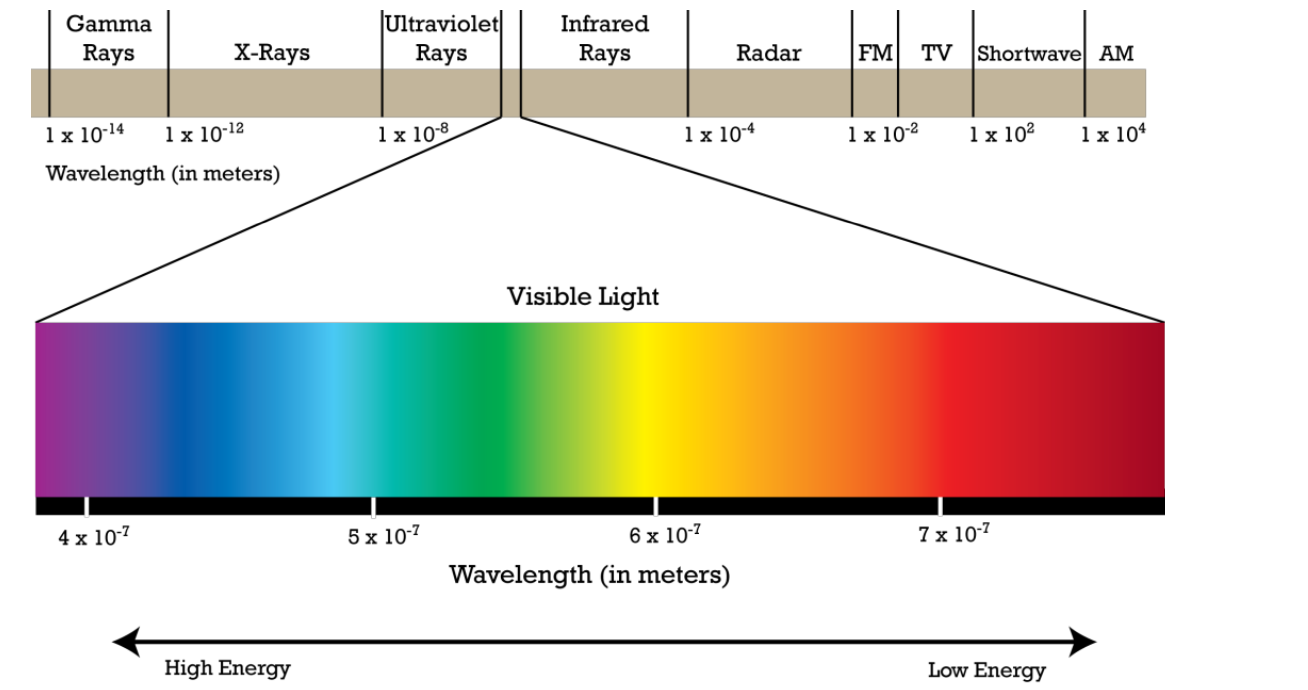
\includegraphics[width=12cm, height=3.5cm] {light.png}
    \caption{Light´s Wavelength\cite{fig1}}
    \label{fig:my_label}
\end{figure}
\\
\\
The figure depicts the wavelength of light in meters along a single axis. The x-axis displays the wavelength in meters, ranging from the shortest to the longest. The representation showcases the varying wavelengths of light and their corresponding values in meters. This information provides an understanding of the differences in wavelength, which is a crucial aspect of light and electromagnetic radiation.\\
\\
The process of the photovoltaic effect is observed when photons, which are the energy carriers of the Sun, are absorbed by solar cells and then transformed into either thermal or electrical energy. The significance of this process lies in its ability to harness the tremendous energy of the Sun for a variety of uses. The structure of solar cells is comprised of a junction between two distinct types of semiconductors, and it is through these semiconductors' properties that the photovoltaic effect is enabled. The following section will delve into the semiconductor world to examine their properties and how they play a role in the functioning of solar cells\cite{CAPV}.


\subsection{Semiconductors}
Atoms consist of a nucleus surrounded by negatively charged electrons. The nucleus is made up of positively charged protons and neutral neutrons. The number of protons in the nucleus determines the type of atom. The number of electrons determines the charge of the atom. And the number of neutrons determines the mass of the atom. Electrons of an isolated atom can have only specific discrete or quantized energy levels  due to the quantum and mechanical nature of the motion of the electrons. When atoms are close together, the electronic energy of individual atoms is changed by the interaction with the other atoms. The electrons of an atom can be excited to a higher energy level by absorbing energy from the environment. The electrons can also be de-excited to a lower energy level by emitting energy into the environment. The energy emitted or absorbed by an atom is equal to the difference in energy between the two energy levels and is called a photon. Thus the energy levels are sorted into energy bands\cite{atom}.\\
\\
The theory of energy bands categorizes the energy levels into energy bands, with the lowest energy band referred to as the valence band and the highest band referred to as the conduction band.
\newpage
\begin{figure}[h!]
    \centering
    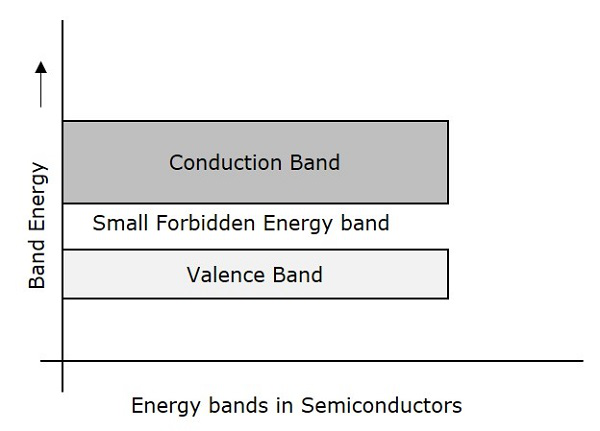
\includegraphics[width=12cm, height=6cm] {semiconductors.png}
    \caption{Bands Energy\cite{semfig}}
    \label{fig:my_label}
\end{figure}
\hfill \break
The figure above represents a band diagram for a semiconductor. A band diagram is a visual representation of the energy levels of electrons in a solid material. The diagram shows the conduction band, the small forbidden energy band, and the valence band. The conduction band is the energy level where electrons are free to move and conduct electricity. The small forbidden energy band is the energy gap between the conduction and valence bands, where no electrons are allowed to exist due to forbidden energy levels. The valence band is the highest energy level occupied by electrons and is where electrons are tightly bound to their parent atoms.\\
\\
The valence band is the band of lower energy electrons.  When electrons in this band are excited, they can jump into the conduction band.  The valence band is just the outermost electron orbital of an atom of any specific material that electrons occupy.\\
\\
The conduction band is the band of higher energy electrons and electrons in it are highly mobile.  When the electrons are in these orbitals, they move freely throughout the material. These are the electrons which carry electricity.\\
\\
The energy difference between the highest occupied energy state of the valence band and the lowest unoccupied state of the conduction band is called the forbidden gap. The forbidden gap is like an electrical energy barrier, as the electrons can not move from the valence band to the conduction band, because it needs energy for this. The gap is called forbidden because the transition from the valence to the conduction band is only possible by absorbing a photon with energy equal to or larger than the energy of the forbidden gap.\\
\\
Semiconductors are materials that are imperfect conductors of electricity, materials that exhibit an intermediate electrical conductivity between conductors such as metals and insulators such as glass. The conductivity of semiconductors is in general lower than the conductors and higher than the insulators. In electrical engineering, semiconductors are used as active components in solid-state devices such as diodes, transistors, and integrated circuits. In a semiconductor, an electric current is favored by two types of carriers: electrons and holes\cite{texbook}.\\
\\
Pure silicon is an intrinsic semiconductor with a gap of about 1.12 eV.  The properties of a semiconductor can be controlled by doping it with impurities. A semiconductor with more electrons than holes is then said to be of type N, and the number of electrons exceeds the number of holes by one electron per dopant atom. A semiconductor with more holes than electrons is said to be of type P, and the number of holes exceeds the number of electrons by one hole per dopant atom\cite{texbook2}.

\subsection{Silicon Doping}
Doping of silicon means that atoms of other elements are added to the silicon lattice. The substitution should be carried out by atoms with three or five valence electrons. There wise the replaced atom creates a hole in the valence band, and consequently, the semiconductor is in a short circuit situation\cite{texbook3}.

\begin{itemize} 
    \item Type N doping : If an atom with five valence electrons is incorporated into the crystal lattice, then this atom will have four bonds covalent and a free electron. This weakly bonded electron can be easily excited to the conduction band. In this kind of material, the number of electrons exceeds the number of holes.
    \item Type P doping : If a trivalent atom is substituted for a silicon atom in the crystal lattice, this atom creates three covalent bonds and one hole. The transition from the valence band to the conduction band is then favored since it decreases the electronic energy. In this kind of material, the number of holes is larger than the number of electrons.
\end{itemize}
\subsection{p-n Junction}
A p-n junction is formed by two adjacent semiconductors of different doping types.
The semiconductor, whose doping is higher in one type of charge carrier, is called a p-type semiconductor, and the semiconductor with an excess of the other type of charge carrier is called an n-type semiconductor.
When a p-type and an n-type semiconductor are brought together, a junction is formed. The junction will contain electrons on one side and holes on the other side. Since electrons and holes are mobile charges, and because they are moving from one side of the junction to the other, there is a spontaneous build-up of the electrical field at the junction.  This creates a potential current of electrons from the n-type material across the metallurgical junction into the p-type material. The term “metallurgical junction” denotes the interface between the n-type and p-type regions. \\
\\
The p-n junction is the key component of a solar cell, which converts the light energy into electricity. When two materials with different electrical conductivities are joined together, the excess electrons from the n-type jump to fill the holes in the p-type, and the holes from the p-type diffuse to the n-type side, leaving the n-side of the junction positively charged, and the p side negatively charged. The negative charge on the p-type side attracts the electrons from the n-type side, and the positive charge on the n-type side attracts the holes from the p-type side. The excess electrons from the n side then flow into a neighboring region called the diffusion region to make an electrically neutral junction. Therefore, a p-n junction behaves like a diode. The diffusion of electrons and holes into the opposite regions is the reason why diodes have asymmetric IV characteristics, i.e., they work as rectifiers. This is the essential property of a solar cell, which makes the production of electricity out of sunlight possible. \\
\\
In the p-type semiconductor, because the doped atoms are of the same type as the majority charge carriers, the doped atoms are not able to accept electrons. Therefore, the doped atoms are called acceptors. In the n-type semiconductor, because the doped atoms are of the same type as the minority charge carriers, the doped atoms are able to accept electrons. Therefore, the doped atoms are called donors\cite{bib1}. \\
\\
\begin{figure}[h!]
    \centering
    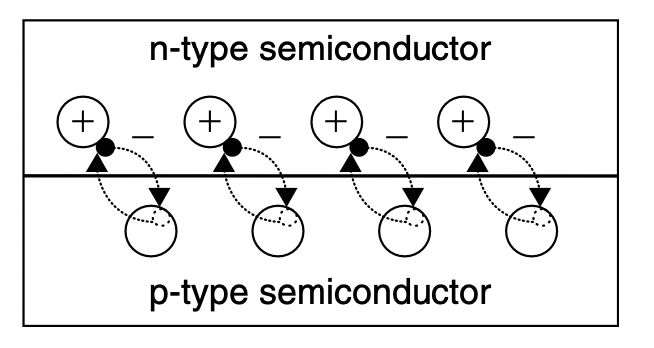
\includegraphics[ height=4cm]{pnj.png}
    \caption{Schematic diagram of a p-n junction\cite{kalogiroubook}}
    \label{fig:my_label}
\end{figure}
\hfill \break
The figure above represents a schematic diagram of a p-n junction. It shows both types of semiconductors, n-type in the part above, and p type in the part below, forming a junction where they meet. The n-type semiconductor is created by doping the semiconductor material with impurities that have one less valence electron than the semiconductor material, and is represented by a negative sign (-). On the other hand, the p-type semiconductor is created by doping the semiconductor material with impurities that have one more valence electron than the semiconductor material, and is represented by a positive sign (+).
\subsection{Photovoltaic Effect}
The photovoltaic effect is a phenomenon discovered in the early 19th century when a French physicist Alexandre-Edmond Becquerel, observed that light falling on certain semiconductor materials creates an electric field in it. When a photon enters a photovoltaic material,  it can be reflected, absorbed, or transmitted depending on the amount of energy this photon has.The energy of the electron is increased by the amount of energy of the photon absorbed by a valence electron of an atom. If the energy of the photon is more than the energy required for the electron to jump to the conduction band, the electron will jump to the conduction band, where it can move freely. In the case of a silicon material, which has an energy gap of 1.12 eV the energy of the photon must be more than this, for the transition of an electron to take place which generate an electrical charge. So the more photons that are absorbed by the solar cell, the more charge is generated. Typically a photovoltaic cell that absorbs 1 J of energy generates 1 C of charge.\\
\\
But even the energy of the photon is very high,  it can make jump only one electron it can make jump only one electron, the rest of the energy is lost as hit. \\
\\
\begin{figure}[h!]
    \centering
    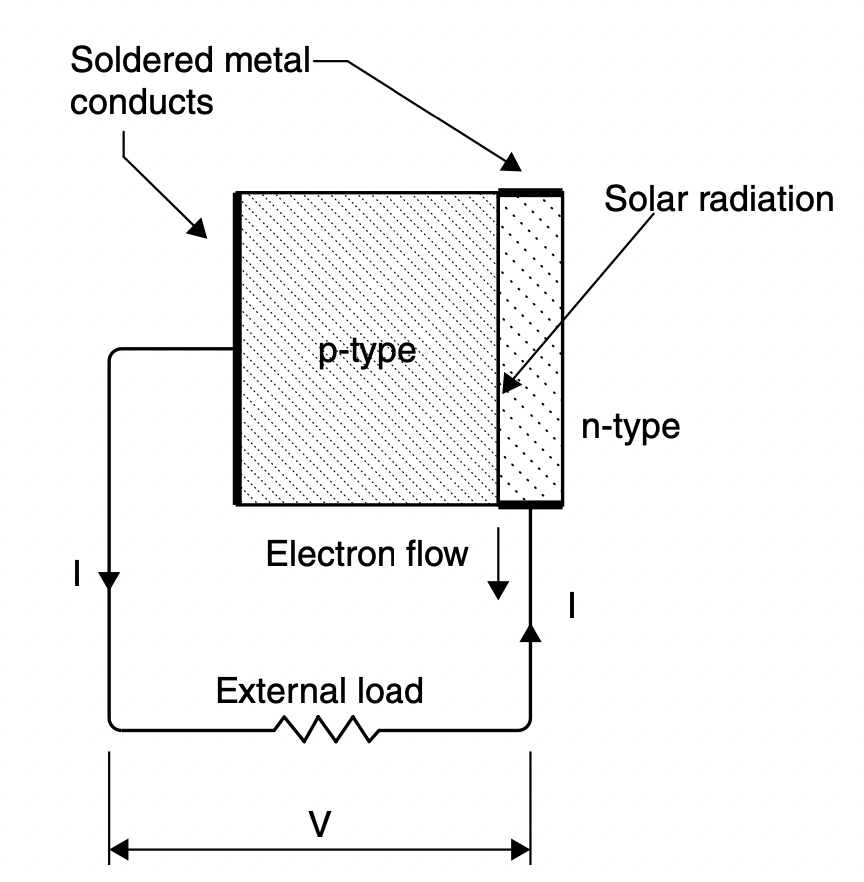
\includegraphics[width=7cm, height=7cm]{phe.png}
    \caption{Photovoltaic effect\cite{kalogiroubook}}
    \label{fig:my_label}
\end{figure}
\hfill \break
The figure above shows a diagram of a typical photovoltaic cell, which consists of two semiconducting materials with different doping levels, typically p-type and n-type silicon. The p-type semiconductor has an excess of positively charged "holes" (vacancies in the valence band) while the n-type semiconductor has an excess of negatively charged electrons.\\
\\
When light (photons) from the sun hits the surface of the photovoltaic cell, it excites electrons in the semiconductors, causing them to move from the n-type semiconductor to the p-type semiconductor. This creates a potential difference or voltage between the two layers of the cell, which causes electrons to flow from the p-type to the n-type semiconductor through an external circuit, generating an electrical current. This flow of electrons creates the electrical power output of the photovoltaic cell.



\subsection{Photovoltaic Cell}
Semiconductors are the electronic components of PV cells. PV cells consist of two or more thin layers of semiconducting material, most commonly silicon, that is prepared in such a way that one part of the atoms of the material becomes negatively charged and the other part becomes positively charged.  Facing the sun to convert directly the sunlight into electricity is known as the Photovoltaic effect. PV cells have been marketed under the name Solar Cells for about a century.\\
\\
Solar cells generate most of their electricity from direct sunlight. However, solar cells typically generate little electricity under clouds or during the night on bright moonlit nights. Individual solar cells typically only generate tiny amounts of electricity. If any of these cells are connected and stacked up, a panel of cells is created. Larger arrays of solar cells provide more electricity and more power than single solar cells.
\subsection{PV Cell Modelization}
A PV generator is mainly an assembly of solar cells, connections, protective parts, and supports. The photovoltaic effect applied into a photovoltaic cell could be represented as the electrical circuit in figure 1 where the diode represents the n-p junction, the current source represents the photon energy, the series resistance  $R_{S}$ represents the resistance inside each cell and the diode´s internal shunt resistance $R_{SH}$.\\
\begin{figure}[h!]
    \centering
    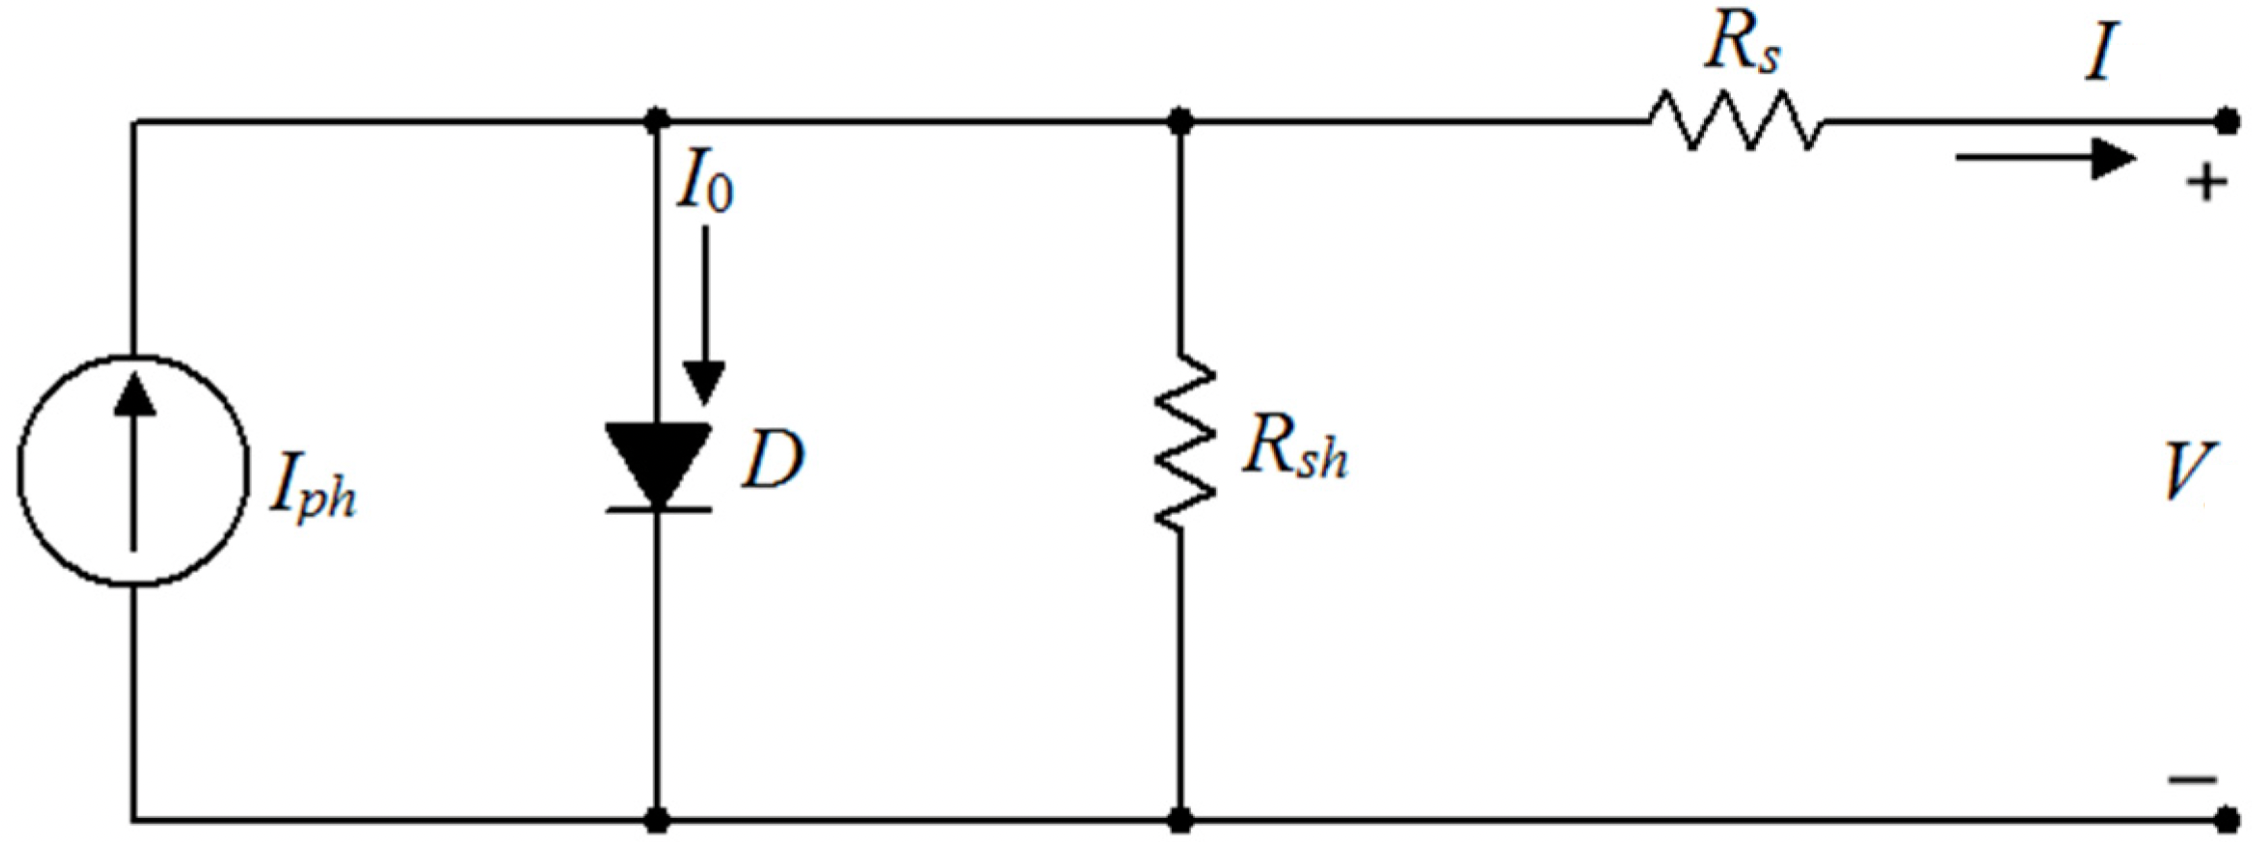
\includegraphics[width=12cm, height=4cm] {fivep.png}
    \caption{Single-diode electrical equivalent circuit of the PV  cell\\ \cite{mughalpaper}}
    \label{fig:my_label}
\end{figure}
\newpage
\hfill \break
The figure above represent a single-diode electrical equivalent circuit of a photovoltaic (PV) cell, it consists of four main components: a current source, a shunt resistance, a series resistance, and a single diode. The current source represents the current generated by the PV cell in response to sunlight, while the shunt resistance represents the current leakage caused by defects in the cell's semiconductor material. The series resistance accounts for the internal resistance of the cell, which can be due to various factors, such as the resistance of the metal contacts and interconnects. Finally, the single diode models the non-linear relationship between the cell's current and voltage, which arises from the properties of the semiconductor material.\\
\hfill \break
The mathematical model of a photovoltaic cell using Kirchhoff law :


\begin{equation}
I = I_{ph} - I_{D} = I_{ph} - I_{s} \{ exp
 \left[  \frac{q(V+IR_{s})}{nk_{B}T_{c}} \right] - 1 \} - \frac{V+IR_{s}}{R_{sh}}
\end{equation}

\begin{enumerate}

    \item $k_{B} : Boltzmann’s gas constant = 1.381 \times 10^{-23}$  J/K
    \item $T_{c}$ : absolute temperature of the cell (K)
    \item V  : voltage imposed across the cell (V)
    \item $I_{s}$ : dark saturation current, which depends strongly on temperature (A)
    \item n : junction idealisation factor
    \item q : electronic charge = 1.602 \times $10^{-19}$ J/V
    \item $R_{s}$ : series resistance ($\Omega$)
    \item $R_{sh}$: Shunt resistance or the parallel resistance ($\Omega$)
\end{enumerate}

\hfill \break
When the cell is short-circuited, the current is at maximum (short-circuit current, $I_{sc}$), and the voltage across the cell is 0.
\hfill \break
And when the PV cell circuit is open,  the voltage is at its maximum (open-circuit voltage, $V_{oc}$), and the current is 0.

\hfill \break
In this subsection, the topic of discussion was the photovoltaic cell modelization. It is considered a vital aspect in determining the behavior and performance of a photovoltaic system. To model the photovoltaic cell accurately, it is necessary to estimate its parameters. That's where the Newton-Raphson method comes into play. This method is a popular numerical method used to estimate parameters in many applications, including photovoltaic cell modelization. In the following section, the application of the Newton-Raphson method to photovoltaic cell modelization will be explored, leading to a more accurate and dependable estimation of the cell parameters.
\subsection{The Newton Raphson Method }
The Newton-Raphson Method is an iterative method used to find the roots of a function. It consists of in estimate of a given function f(x) with an initial guess. It´s a very simple method, but it is very effective. The method is based on the fact that the tangent line to a function at a point is a good approximation to the function itself\cite{NRM}.\\
\\
The method is obtained through the Taylor series
expansion in (x -− $x_{0}$) given below:\\
\begin{equation}
f(x) = f(x_{0}) + f'(x_{0})(x-x_{0})  + \frac{1}{2} f''(x_{0})(x-x_{0}) + ... = 0
\end{equation}
\\
It is said that when the initial guess is close to the real root of the equation, the value of (x-$x_{0}$) is small, and only the first terms are significant for calculating the root, based on $x_{0}$. By cutting off the series in the second term, the general formula of the Newton-Raphson method can be derived\cite{nr2}.

\begin{equation}
x_{1} = x_{0} - \frac{f(x_{0})}{f'(x_{0})}
\end{equation}
\\
Therefore, given $x_{n}$, the point $x_{n+1}$ will be obtained by intersecting the tangent line at f(x) in $x_{n}$ with the x axis.

\begin{equation}
x_{n+1} = x_{n} - \frac{f(x_{n})}{f'(x_{n})}
\end{equation}
\\
The convergence of the Newton Raphson Method is
guaranteed for a certain interval [a,b] containing the root of f(x), provided that f(x) and f'(x) are continuous in this interval and that f($\alpha$) = 0, where $\alpha$ is the root of f(x).

\begin{figure}[h!]
    \centering
    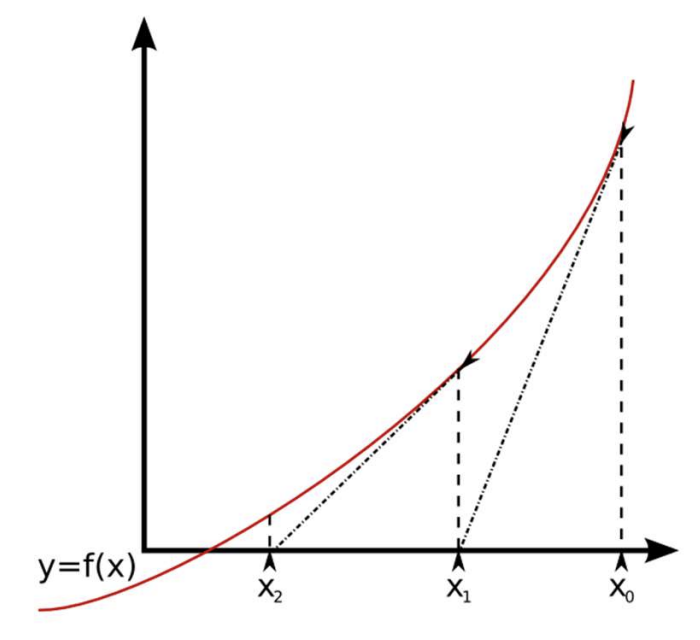
\includegraphics[width=9cm, height=4cm] {d.png}
    \caption{Illustration of the Newton Raphson Method\cite{nr2}.}
    \label{fig:my_label}
\end{figure}
\hfill \break
The x-axis of the graph above represents the iteration number, while the y-axis represents the error between the current estimate of the root and the actual root. It shows a curve that starts at an initial error value $x_{0}$ and decreases as the algorithm progresses through its iterations. While the curve approach zero, the algorithm converges on the root.
\subsection{Theoretical Simulation}
Using \begin{math} I_{ph}=0.8 A, I_{s}=10^{-5}A, T_{c}=198,5 K, n=1.5, R_{s}=0.01 \Omega, R_{sh}=50 \Omega, \end{math} the following graphics (Figure 3 and 4) of current depending on voltage and power depending on voltage has been reached.
\begin{figure}[h!]
    \centering
    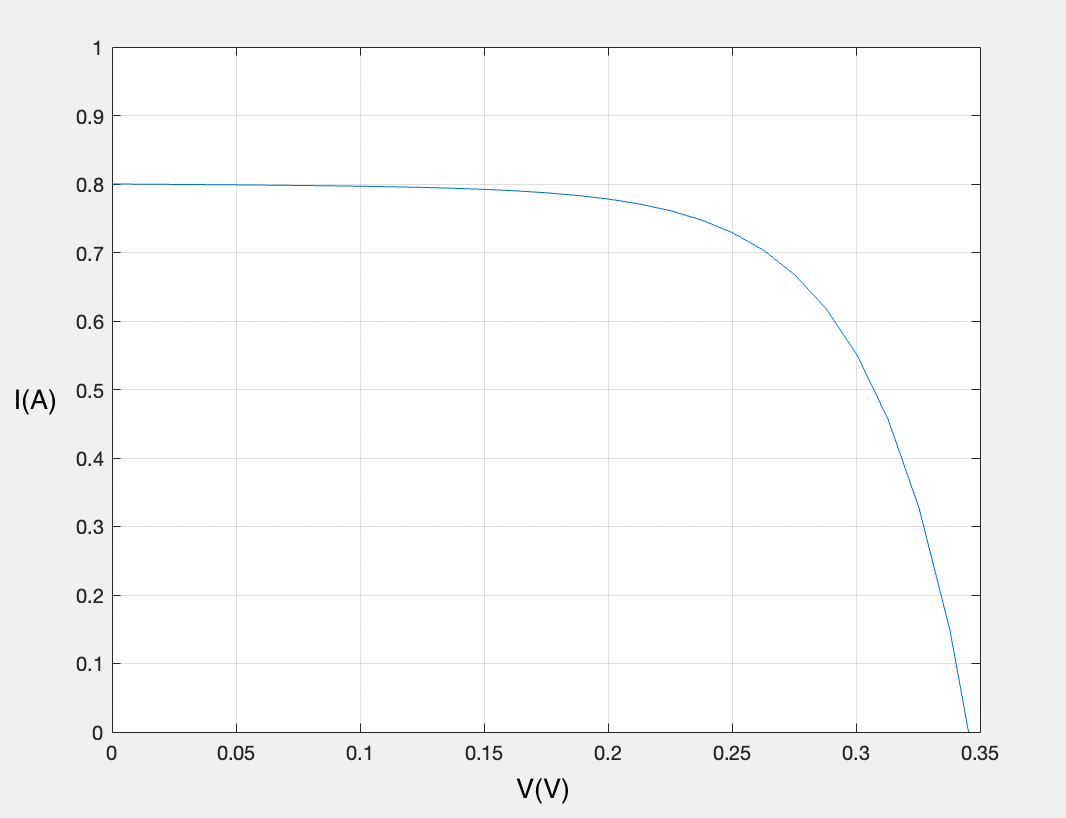
\includegraphics[width=9cm, height=4cm] {IV.png}
    \caption{Representative current-voltage curve for photovoltaic cells}
    \label{fig:my_label}
\end{figure}

\hfill \break
Figure 2.7 is a graphical representation of the relationship between the current generated by the PV cell and the voltage applied across it. The curve is used to determine the operating point of the PV cell and to calculate its efficiency. The current-voltage (I-V) curve is created by plotting the current generated by the cell against the voltage applied to it. The I-V curve is unique for each PV cell and is dependent on various factors such as temperature, light intensity, and material quality.\\
\\
The I-V curve's shape exhibits a sharp rise in current at lower voltage levels, followed by a gradual decline as voltage increases. At the point where the curve reaches its highest value, it is designated as the maximum power point (MPP). The MPP is considered the optimal operating point for the PV cell, as it corresponds to the maximum power that the cell can generate given specific circumstances\\
\\
Shunt resistance is usually much bigger than a load resistance, whats means that less power is dissipated internally within the cell.Therefore, by ignoring these two resistances, the equation become:

\begin{equation}
I = I_{ph} - I_{D} = I_{ph} - I_{s} \{ exp
 \left[  \frac{qV}{nk_{B}T_{c}} \right] - 1 \}  - \frac{V}{R_{sh}}
\end{equation}
\\
The output power, P, from a photovoltaic cell is given by
\begin{equation}
P = IV
\end{equation}
\begin{equation}
P =  \{I_{ph} - I_{s} \{ exp
 \left[  \frac{qV}{nk_{B}T_{c}} \right] - 1 \} - \frac{V}{R_{sh}} \} V
\end{equation}
\begin{figure}[h!]
    \centering
    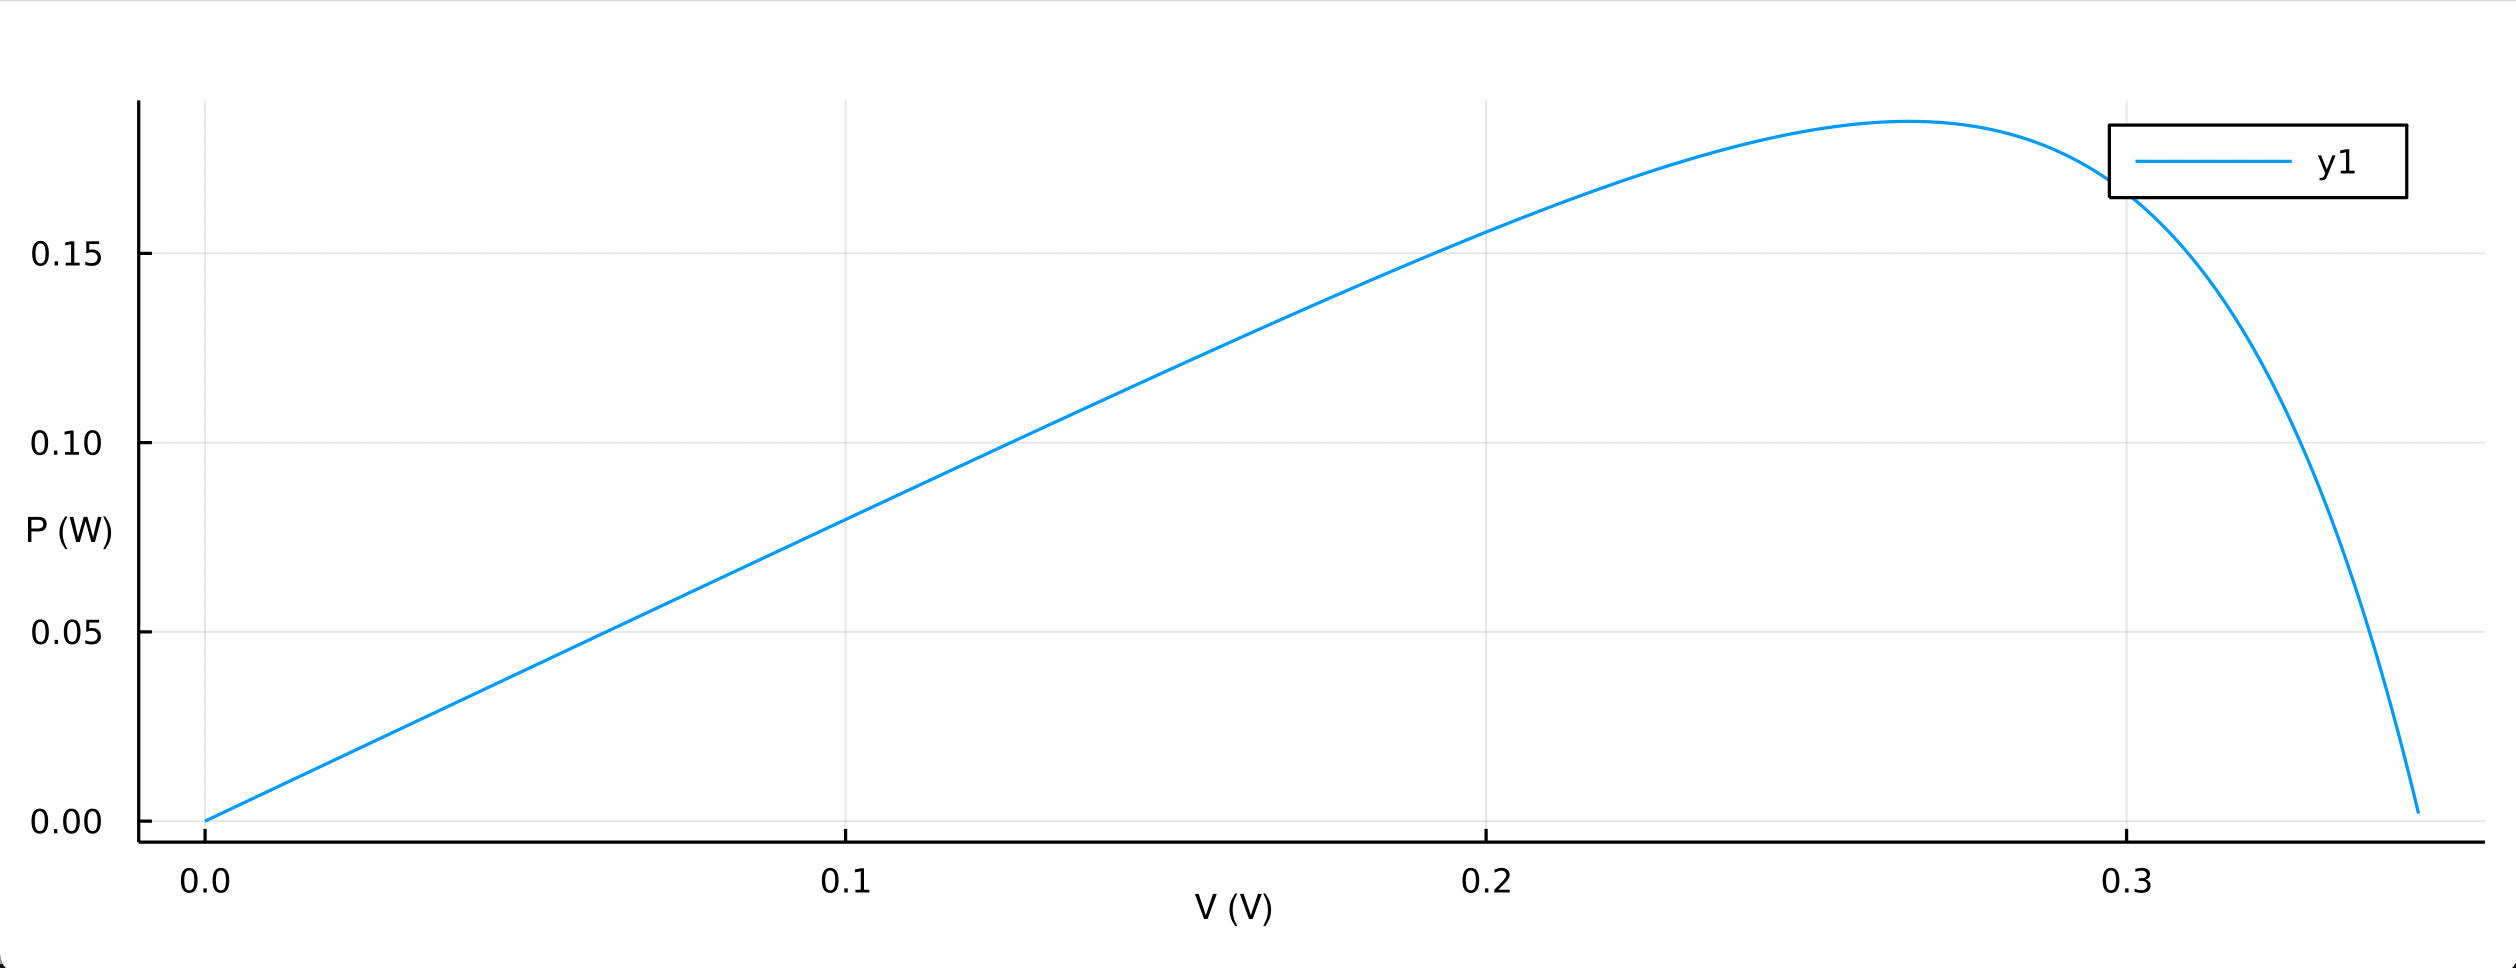
\includegraphics[width=9cm, height=4cm] {PV.png}
    \caption{Representative power-voltage curve for photovoltaic cells}
    \label{fig:my_label}
\end{figure}

\hfill \break
Figure 2.8 is a graphical representation of the output power of a photovoltaic cell as a function of the voltage. This curve is typically plotted using the characteristic values of the photovoltaic cell, such as the photocurrent, the saturation current, the temperature coefficient, and the shunt resistance. The curve is important because it allows us to determine the maximum power point (MPP), which is the operating point of the photovoltaic cell that produces the maximum output power. This information is crucial in designing photovoltaic systems as it helps to optimize the system's efficiency.
\subsection{Simulation With Noise}

Theoretical values often yield results that differ from experimental findings. To achieve results that more closely reflect reality and follow a normal distribution, a degree of randomness with a certain standard deviation can be introduced.
The graphics shown below (Figure 6 and 7) utilize a standard deviation of 2.5\%:
\begin{figure}[h!]
    \centering
    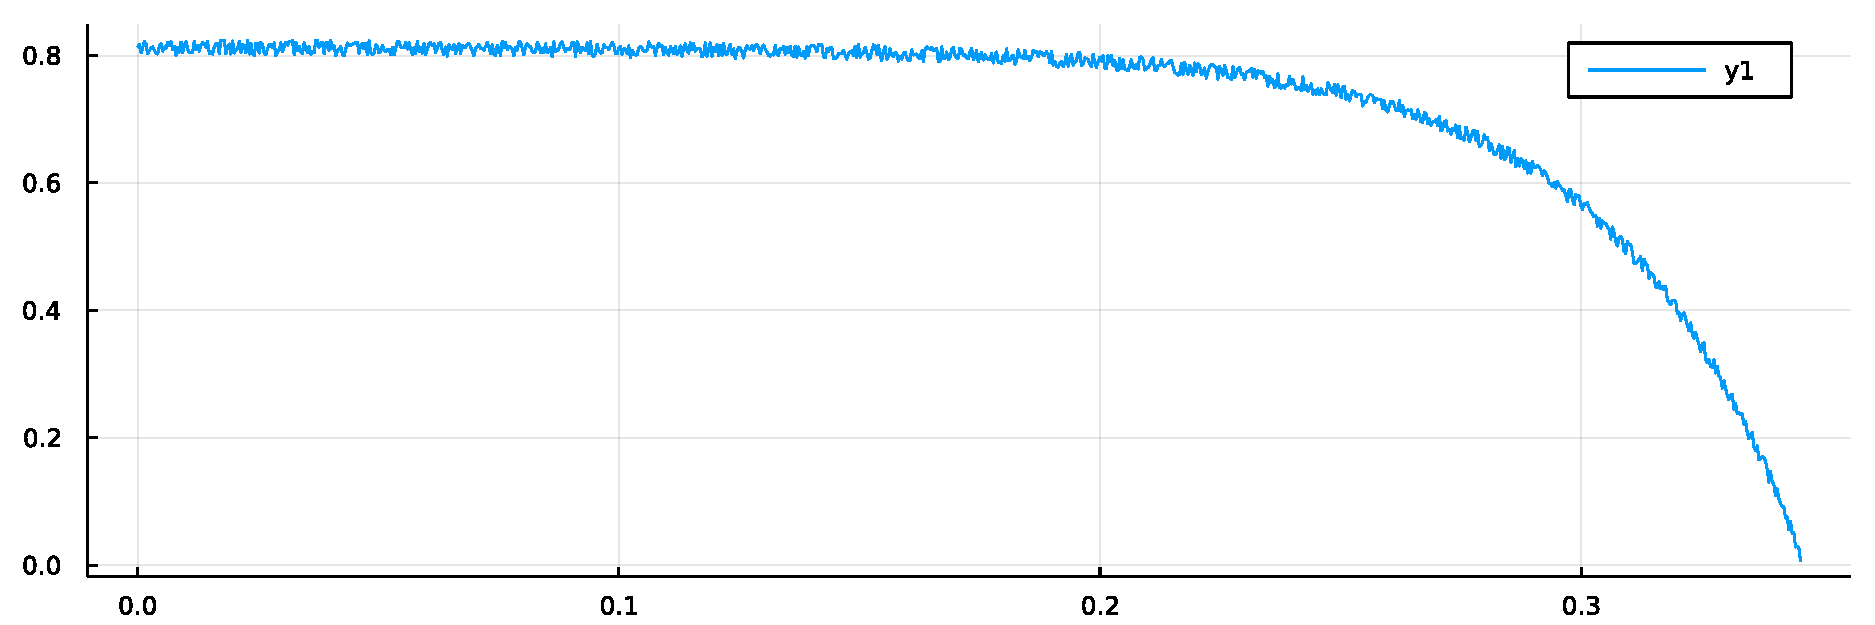
\includegraphics[width=9cm, height=4cm] {test.pdf}
    \caption{Representative current-voltage curve for photovoltaic cells with noise}
    \label{fig:my_label}
\end{figure}

\hfill \break
Figure 2.9 shows the relationship between the current and voltage of a photovoltaic cell when there is external interference, such as electrical noise, that affects the performance of the cell. The presence of noise can cause fluctuations in the current-voltage curve, resulting in deviation from the expected results. This deviation can be seen as variations in the slope or shape of the curve, which can have a significant impact on the output power of the photovoltaic cell. It is therefore important to consider the effects of noise in photovoltaic cell modeling and simulation to accurately predict the performance of the cell in real-world applications.

\begin{figure}[h!]
    \centering
    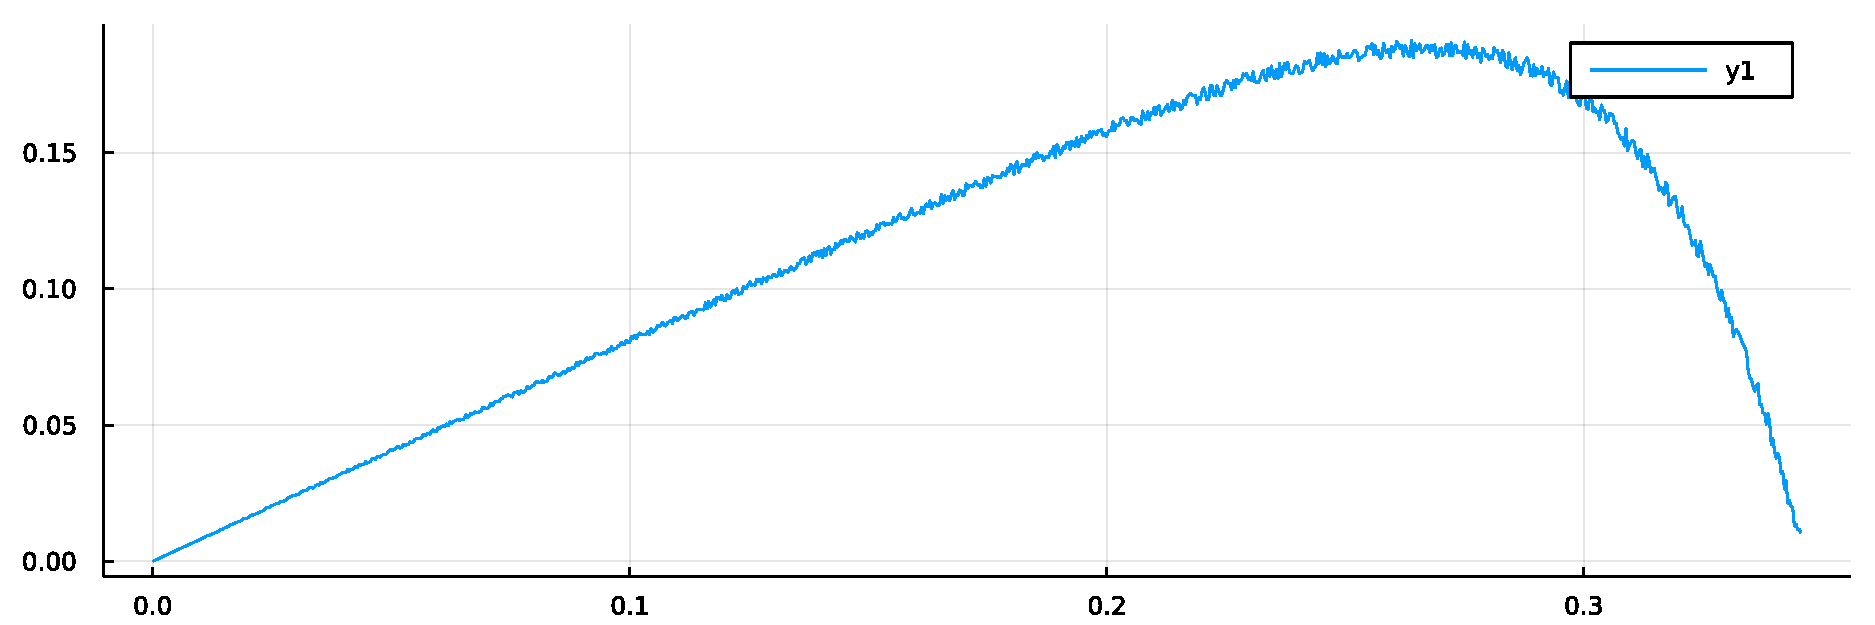
\includegraphics[width=9cm, height=4cm] {sd.pdf}
    \caption{Representative power-voltage curve for photovoltaic cells with noise}
    \label{fig:my_label}
\end{figure}
\newpage
\hfill \break
Figure 2.10 shows the relationship between the power and voltage of a photovoltaic cell, with added noise. The curve shows how the power output of the photovoltaic cell varies with the voltage, while taking into account the effect of noise. 
\hfill \break
The new findings, while not deviating significantly from theoretical values, are more realistic. The results reveal that the region of the curve most impacted by the introduced randomness is the area of the MMP.\\
\\
Despite the simulation incorporating randomness, the measurements obtained are not entirely indistinguishable from real-world data. To enhance the accuracy of the results, it is recommended to process them through an Analog to Digital Converter (ADC)\cite{texbook4}.
\subsection{Analog To Digital Converter}
An analog-to-digital converter is a device that converts an analog signal, such as those captured by microphones, into a digital signal. This type of electronic device is commonly used in electronic devices. The resolution of an ADC differs from one to another, and its complexity is also decided to depend on the complexity of the operation. An ADC converts continuous time and amplitude into digital time and amplitude.
The process is showed in the Flow Chart below in figure 2.11:
\begin{figure}[h!]
    \centering
    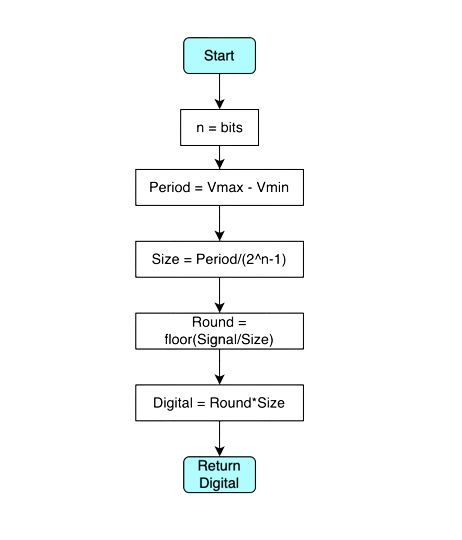
\includegraphics[width=6cm, height=8cm] {ADC.png}
    \caption{ADC Flowchart}
    \label{fig:my_label}
\end{figure}
\hfill \break
The ADC flowchart describes a step-by-step process for converting an analog signal into a digital signal using an Analog-to-Digital Converter (ADC). It begins by determining the number of bits that will be used to represent the digital signal. Next, the voltage range of the analog signal is determined by subtracting the maximum voltage from the minimum voltage, and this value is assigned to a variable called "Period". The voltage range is then divided into equal intervals, each of which is assigned a value called "Size". The analog signal is then divided into intervals of size, and each interval is assigned a digital value. The digital value is obtained by multiplying the rounded interval value with the interval size. Finally, the digital value obtained is returned as the output of the ADC conversion process. Overall, the ADC flowchart provides a systematic and logical approach for converting analog signals into digital signals with a fixed number of bits, a defined voltage range, and a specific resolution.
\section{Analysis of I-V and P-V characteristics}
\subsection{Effect of Solar Radiation Variation}

The variation of both I-V and P-V curves will be examined by altering the solar radiation values. Specifically, three distinct values (500, 1000, and 2000 W/$m^2$) will be utilized for this purpose.\\

\begin{figure}[h!]
  \centering
  \subfloat[I-V characteristics]{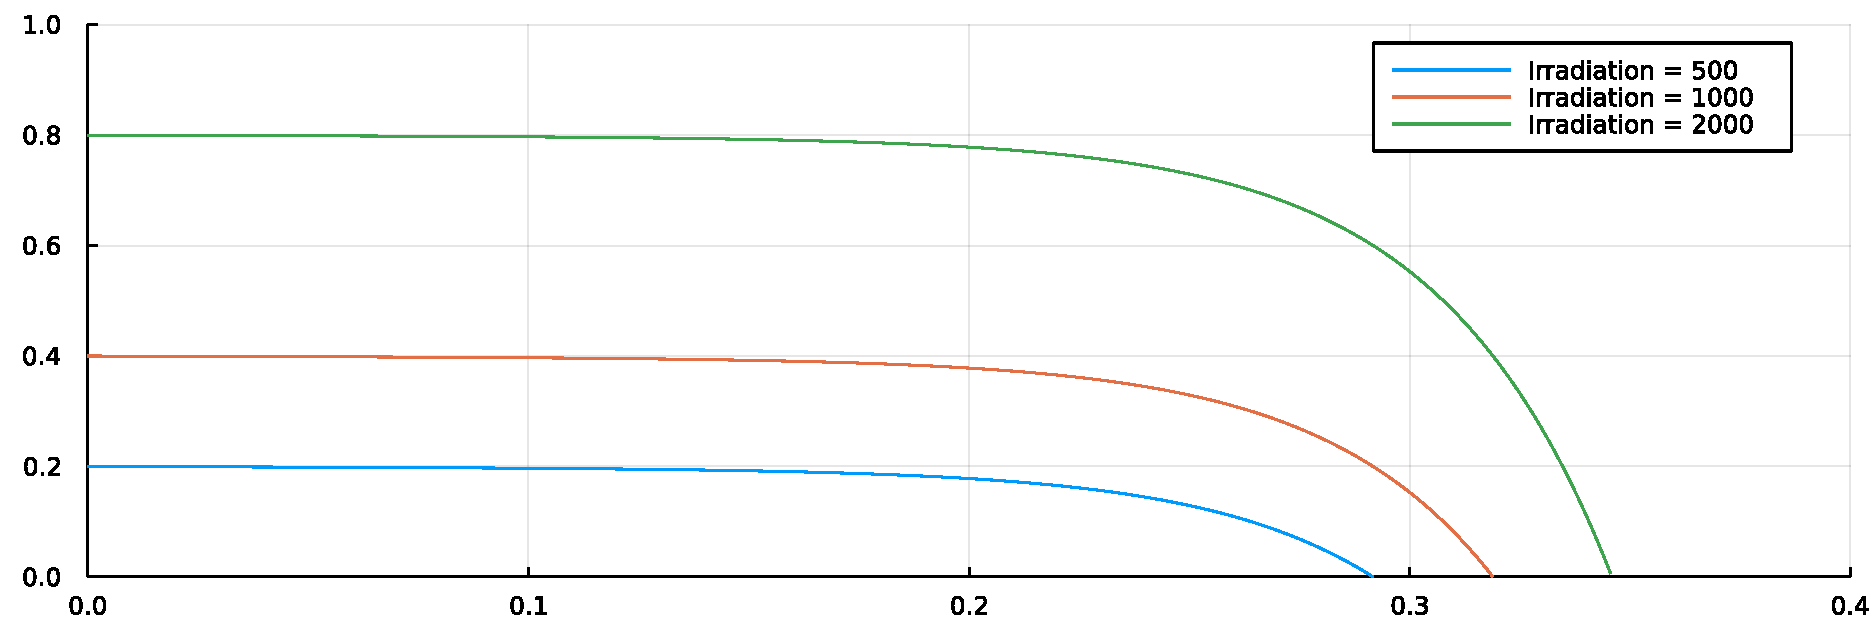
\includegraphics[width=6cm, height=4cm]{SRIV.pdf}\label{fig:f1}}
  \hfill
  \subfloat[P-V characteristics]{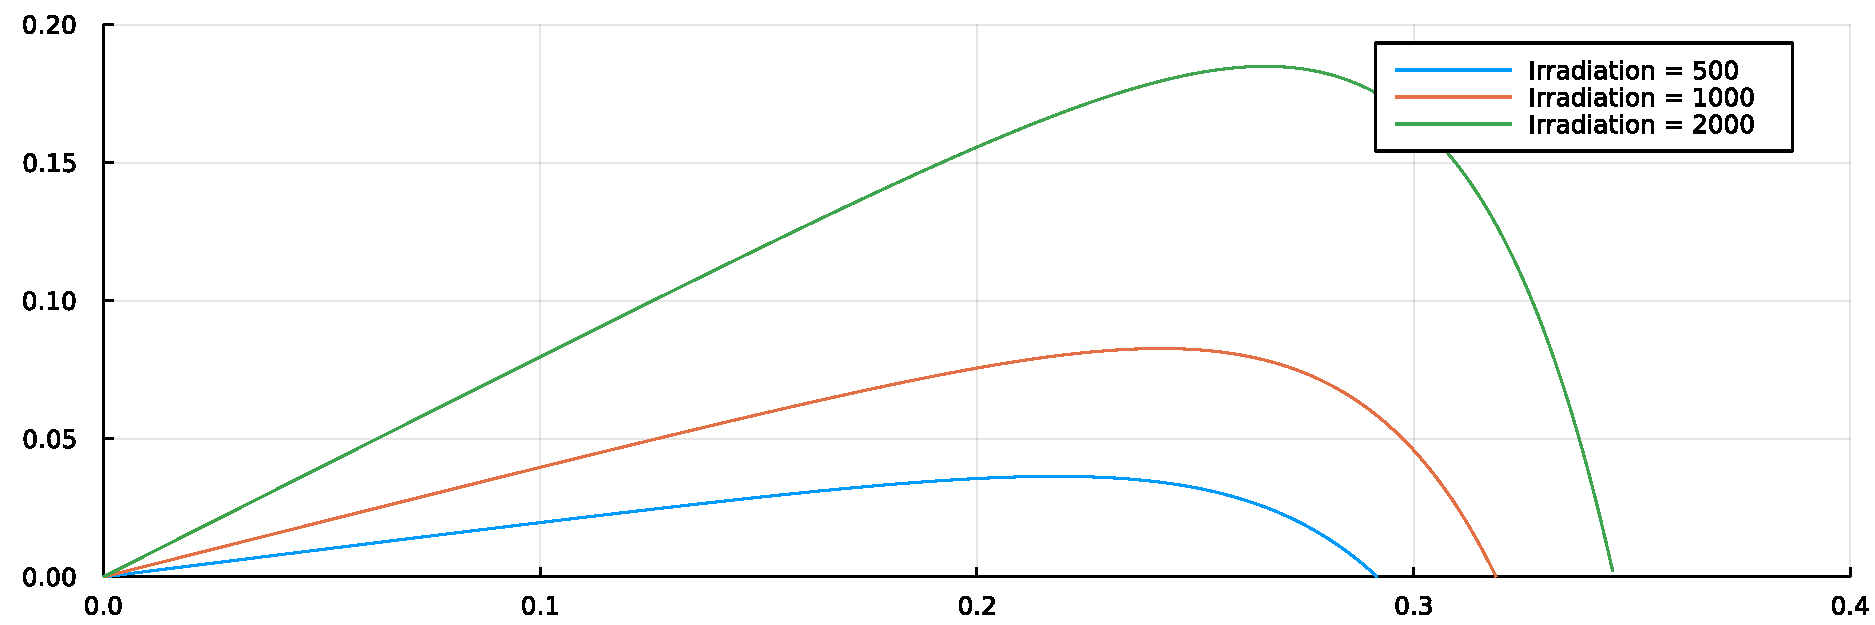
\includegraphics[width=6cm, height=4cm]{SRPV.pdf}\label{fig:f2}}
  \caption{Characteristics with varying solar irradiation}
\end{figure}

The figure presented above demonstrates that:
\begin{itemize}
    \item In a current-voltage curve (I-V), the increase of solar radiation is accompanied by a logarithmic increase of short circuit current  ($I_{sc}$) and a linear increase in open circuit voltage ($V_{oc}$) \newpage
    \item  An increase in solar radiation from 500 to 1000 W/$m^2$ resulted in a 0.2 A increase in $I_{sc}$ and a 0.01 V increase in $V_{oc}$, while an increase in solar radiation from 1000 to 2000 W/$m^2$ resulted in a 0.4 A increase in $I_{sc}$ and a 0.025 V increase in $V_{oc}$
    \item In a power-voltage curve (P-V), the increase in solar radiation is accompanied by a logarithmic increase in maximum power
    \item  An increase in solar radiation from 500 to 1000 W/$m^2$ resulted in a 0.0422 W increase in $P_{max}$ and a 0.01 V increase in $V_{oc}$, while an increase in solar radiation from 1000 to 2000 W/$m^2$ resulted in a 0.0971 W increase in $P_{max}$ and a 0.025 V increase in $V_{oc}$
\end{itemize}

\subsection{Effect of Cell Temperature Variation}

The variation of both I-V and P-V curves will be examined by altering the temperature values. Specifically, three distinct values (20, 40, and 60 °C) will be utilized for this purpose.

\begin{figure}[h!]
  \centering
  \subfloat[I-V characteristics]{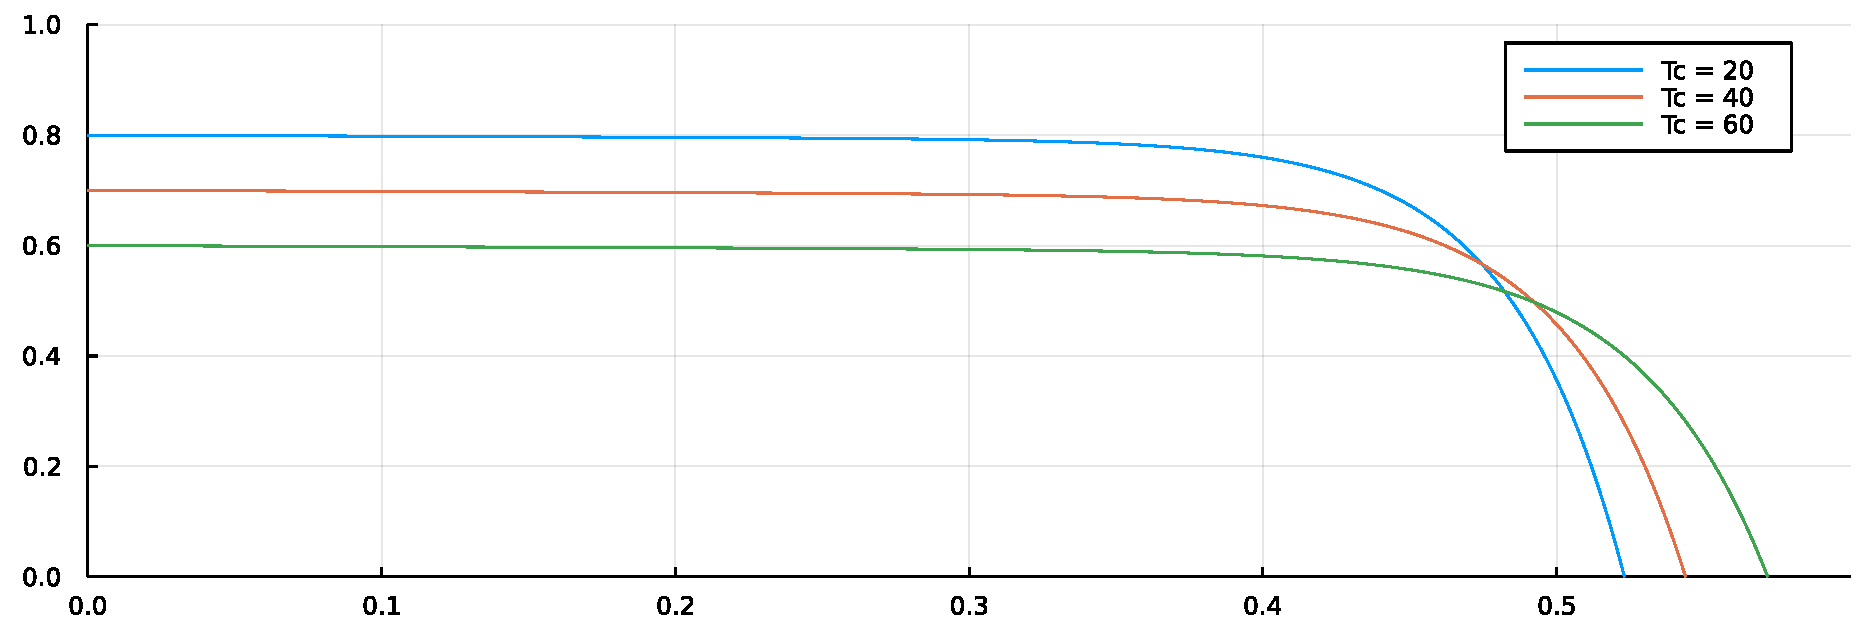
\includegraphics[width=6cm, height=4cm]{newIV.pdf}\label{fig:f1}}
  \hfill
  \subfloat[P-V characteristics]{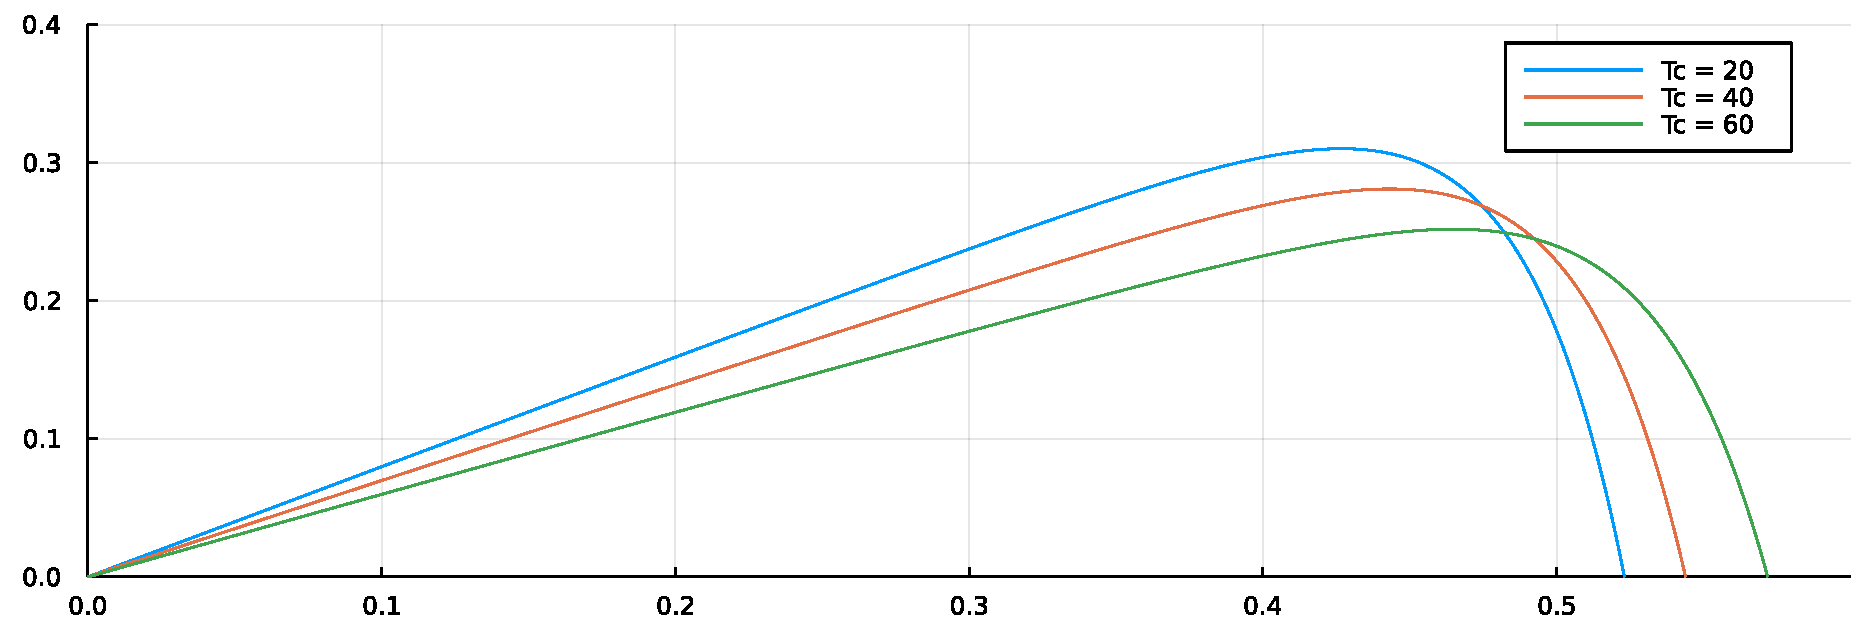
\includegraphics[width=6cm, height=4cm]{newPV.pdf}\label{fig:f2}}
  \caption{Characteristics with varying cell temperature}
\end{figure}


The figure above displays that:
\begin{itemize}
    \item The increase in cell temperature is accompanied by a linear decrease in open circuit voltage and an increase in short-circuit current
    \item  An increase in cell temperature from 20 to 40 °C resulted in a 0.1 A increase in $I_{sc}$ and a 0.01 V decrease in $V_{oc}$. On the other hand, an increase in cell temperature from 40 to 60 °C resulted in a 0.1 A increase in $I_{sc}$ and a 0.005 V decrease in $V_{oc}$
    \item The increase in cell temperature is accompanied by a linear decrease in maximum power \newpage
    \item  An increase in cell temperature from 20 to 40 °C resulted in a 0.02 W decrease in $P_{max}$ and a 0.03 V decrease in $V_{oc}$. Moreover, an increase in cell temperature from 40 to 60 °C resulted in a 0.017 W decrease in $P_{max}$ and a 0.02 V decrease in $V_{oc}$
\end{itemize}
\subsection{Effect of Shunt Resistance Variation}
The variation of both I-V and P-V curves will be tested by changing the shunt resistance values, using three different values of 10, 50, and 100 $\Omega$.

\begin{figure}[h!]
  \centering
  \subfloat[I-V characteristics]{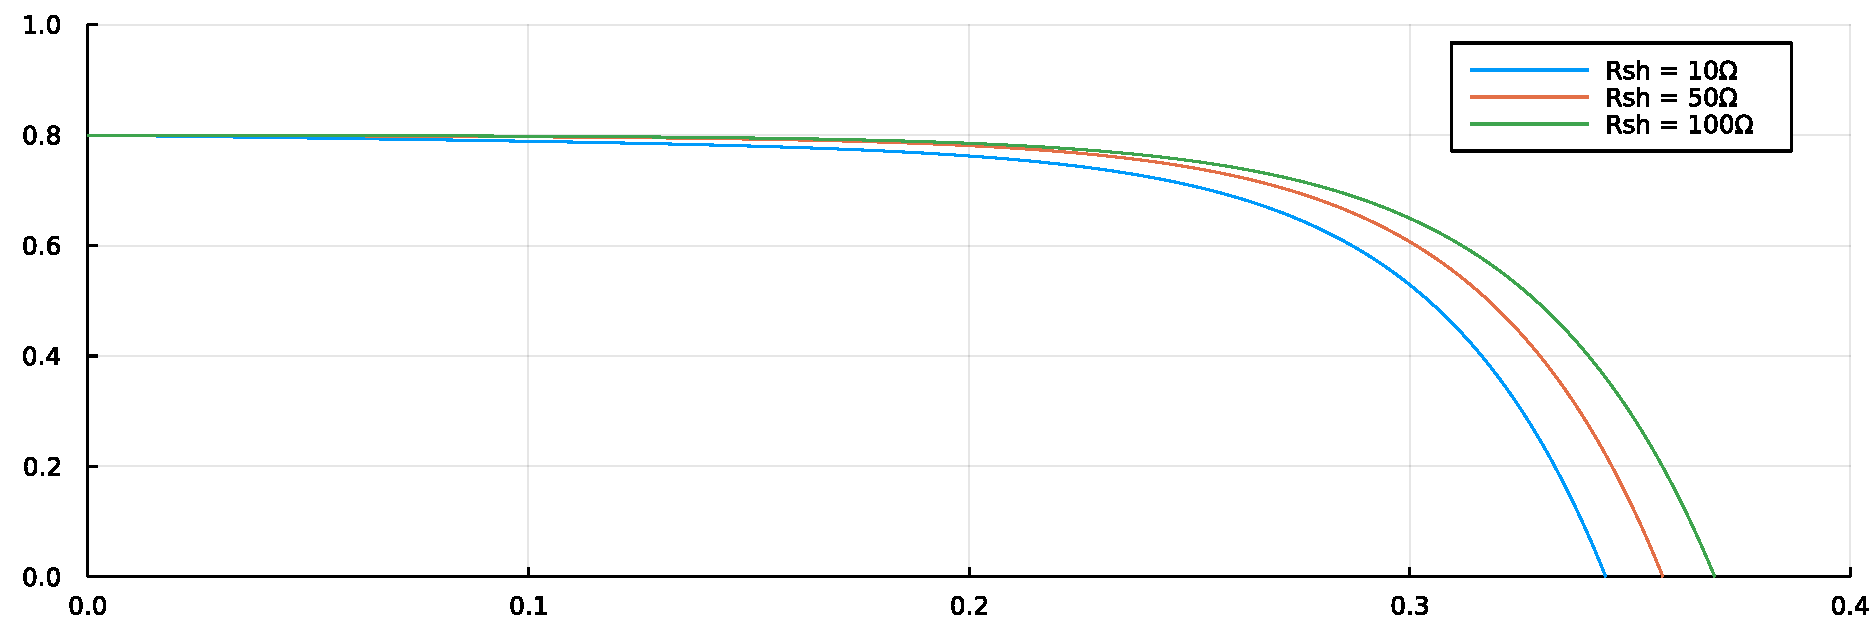
\includegraphics[width=6cm, height=4cm]{RshIV.pdf}\label{fig:f1}}
  \hfill
  \subfloat[P-V characteristics]{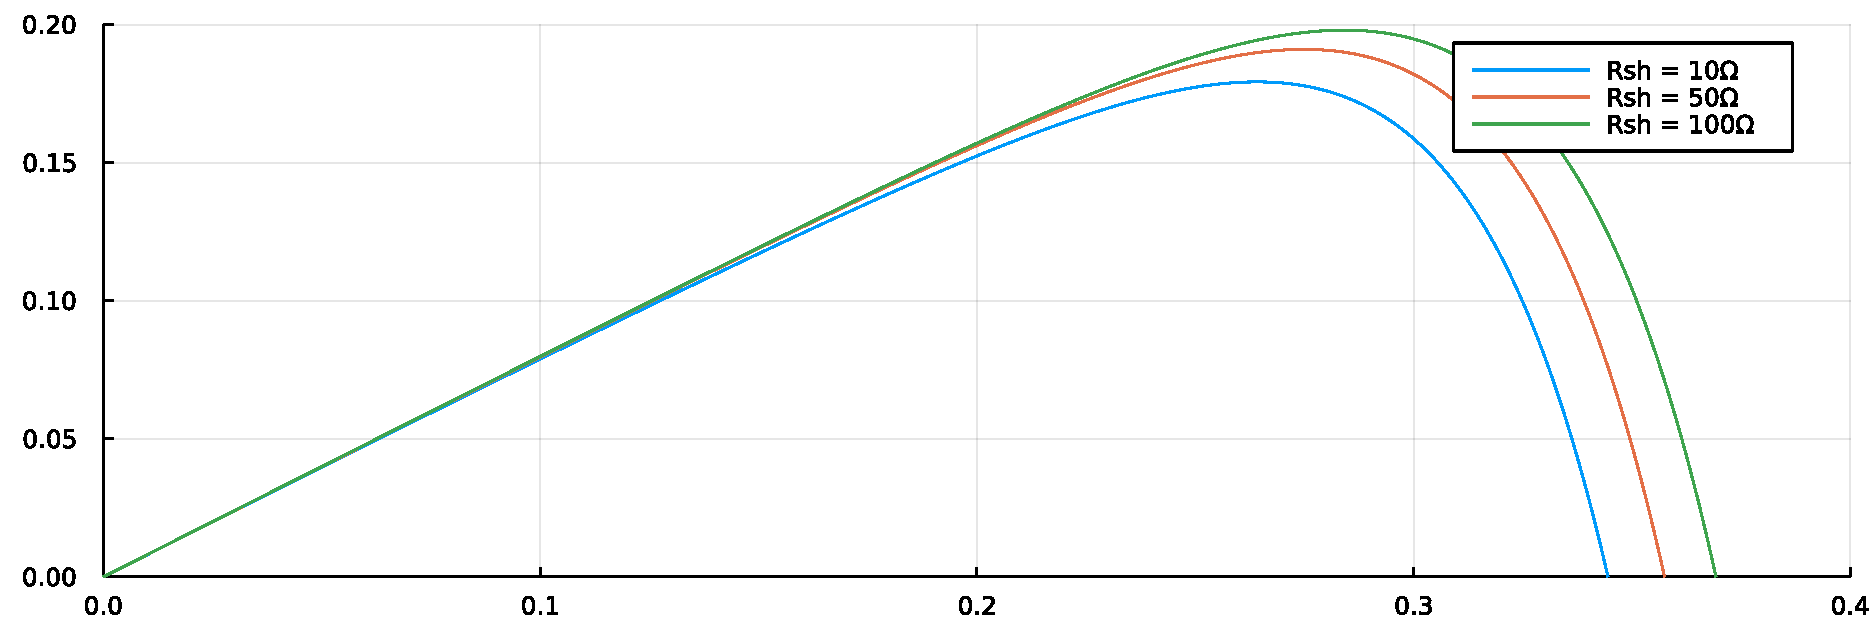
\includegraphics[width=6cm, height=4cm]{RshPV.pdf}\label{fig:f2}}
  \caption{Characteristics with varying Shunt Resistance}
\end{figure}

\hfill \break
The figure above shows that:
\begin{itemize}
    \item The increase of shunt resistance is accompanied by a linear increase in open circuit voltage and stability in short circuit current
    \item  Shunt resistance is used to measure high currents and it is connected in parallel. With the increase of shunt resistance, both open circuit voltage, and maximum power
    \itemIn both the current-voltage (I-V) and power-voltage (P-V) curves, it can be observed that increasing the shunt resistance results in a decrease in the drop of the functions.
\end{itemize}

\subsection{Effect of Diode Reverse Saturation Current Variation}

The variation of both the current-voltage (I-V) and power-voltage (P-V) curves will be tested by changing the diode reverse saturation current $I_{s}$ values. In this case, three different values will be used: 1, 20, and 100 nA.

\begin{figure}[h!]
  \centering
  \subfloat[I-V characteristics]{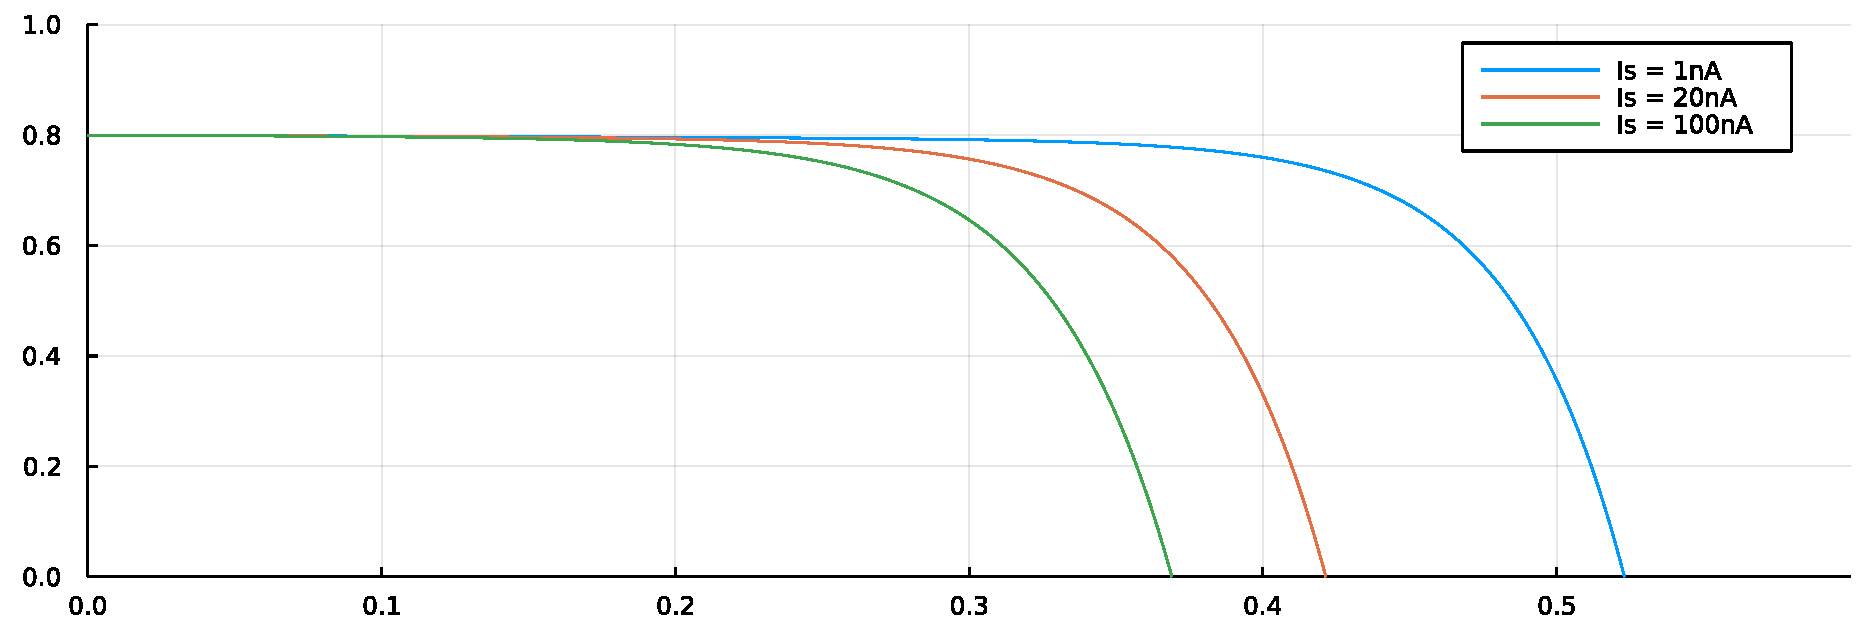
\includegraphics[width=6cm, height=4cm]{IsIV.pdf}\label{fig:f1}}
  \hfill
  \subfloat[P-V characteristics]{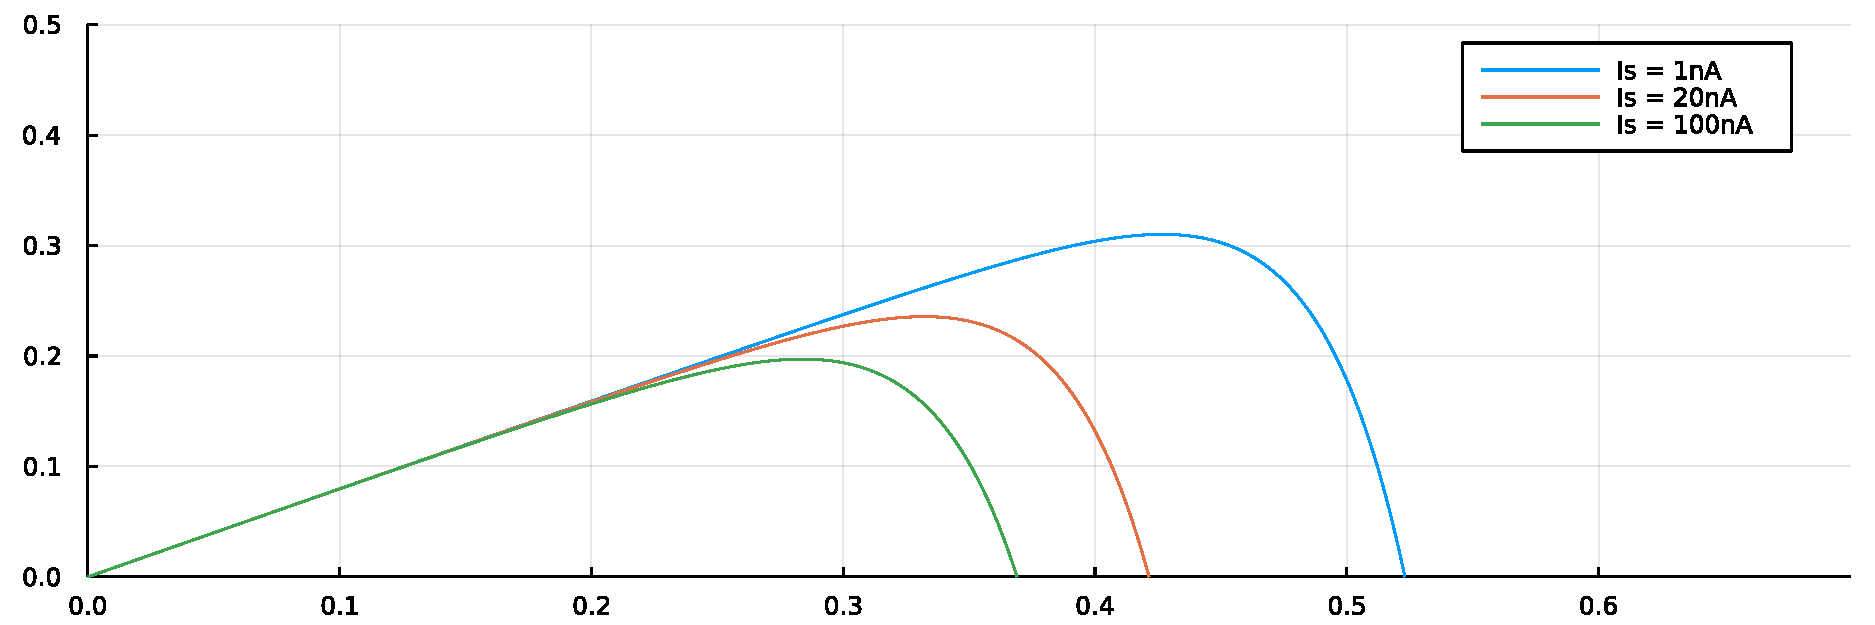
\includegraphics[width=6cm, height=4cm]{IsPV.pdf}\label{fig:f2}}
  \caption{Characteristics with varying diode reverse saturation current}
\end{figure}

\newpage
\hfill \break
The figure above illustrates that:
\begin{itemize}
    \item The increase of diode reverse saturation current ($I_{s}$) is accompanied by a logarithmic decrease in open circuit voltage and stability in short circuit current 
    \item The increase of diode reverse saturation current ($I_{s}$) is also accompanied by a logarithmic decrease in maximum power output
    \item In both the current-voltage (I-V) and power-voltage (P-V) curves, it can be observed that increasing the shunt resistance results in an increase in the drop of the functions.
\end{itemize}


\section{Five Parameters Model}

This photovoltaic cell is characterized by its equivalent plan consisting of a constant current source representing a solar cell's photocurrent. This current varies according to the temperature of the photovoltaic cells and the irradiance level to which they are subjected. This current is connected in parallel to a diode that has an ideality factor n to account for the recombination of electrons in the depletion region of a p-n junction solar cell.  In other words, the voltage drop across the p-n junction of a solar cell. This model accounts for the losses due to the module´s series and parallel resistance. The serial resistance is due to the contact resistance and the resistance of the conductors and the shunt´s resistance is due to resistance in the electrical connection of the solar cells. \\
\newpage
The equivalent circuit of this model is represented in the figure bellow:\\


\begin{figure}[h!]
  \centering
    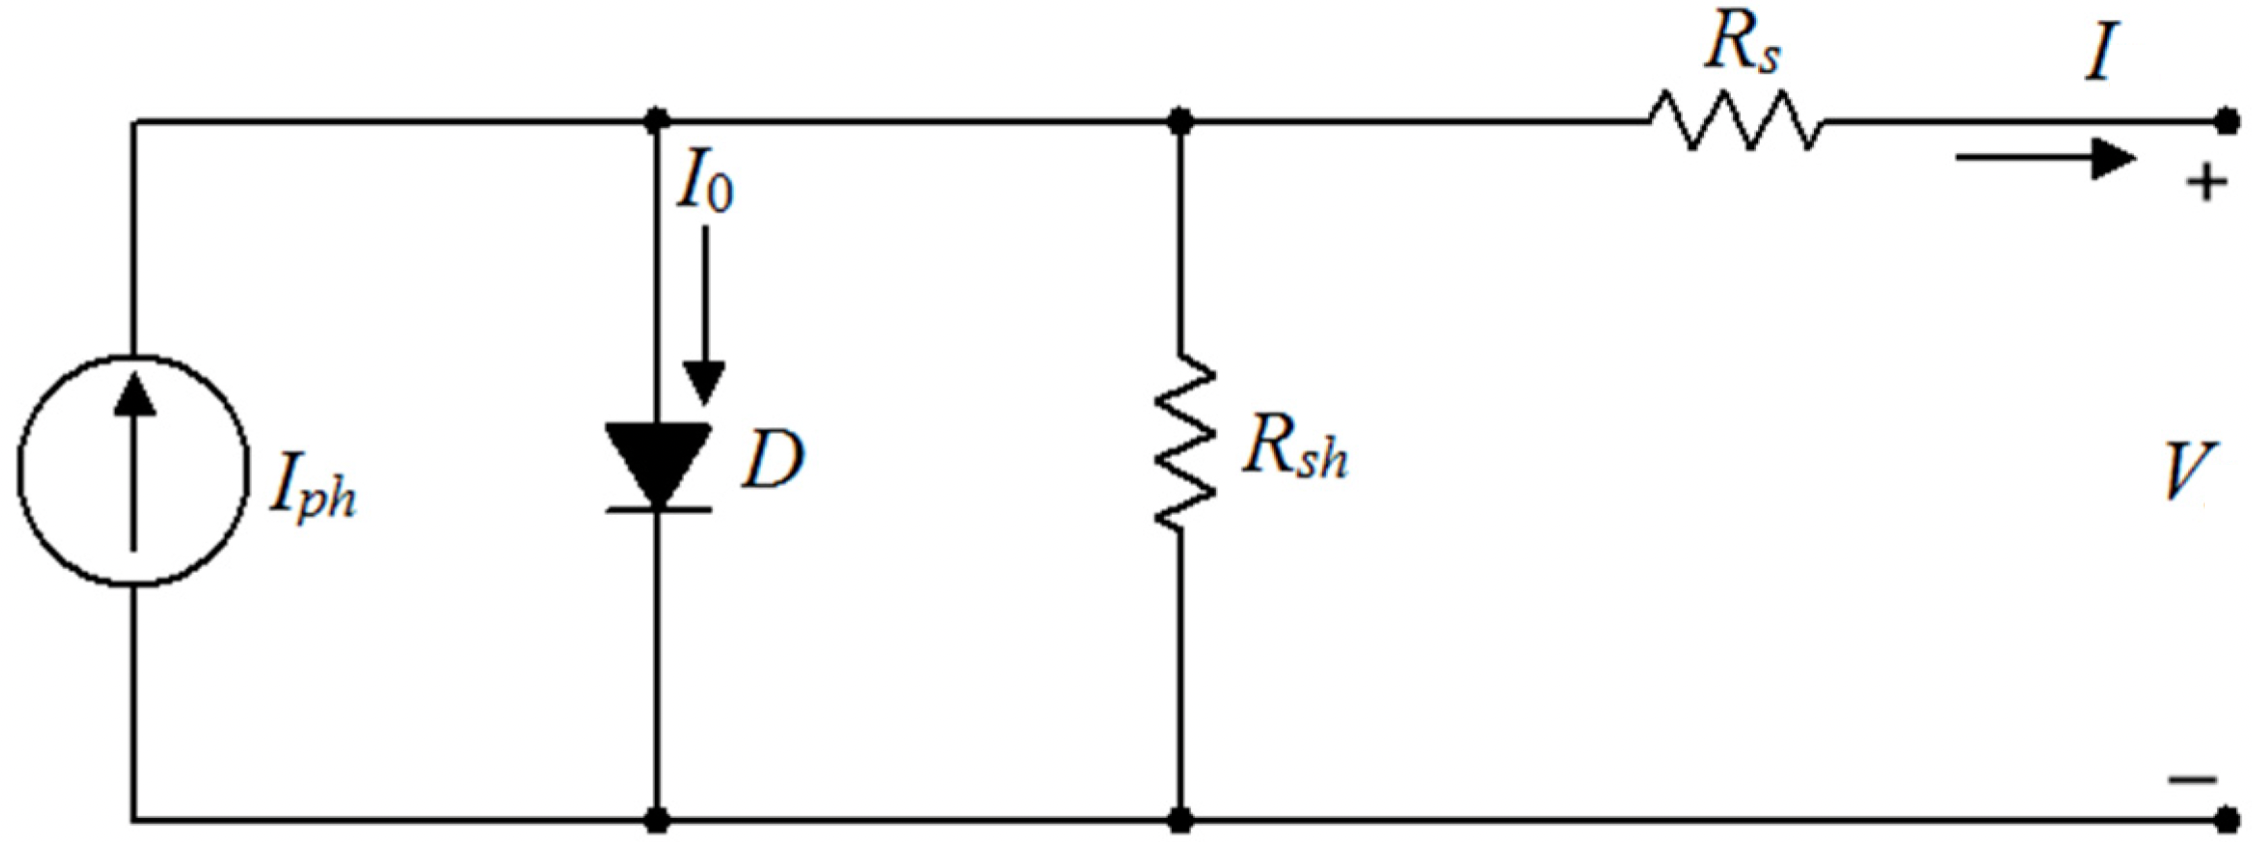
\includegraphics[width=8cm, height=3cm] {fivep.png}
    \caption{Single diode model \cite{kalogiroubook}}
    \label{fig:my_label}
\end{figure}
\hfill \break
The mathematical model is given by :
\begin{equation}
I = I_{ph} - I_{s} \{ exp
 \left[  \frac{q(V+IR_{s})}{nk_{B}T_{c}} \right] - 1 \} - \frac{V+IR_{s}}{R_{sh}}
\end{equation}
\\
Its an equation with 2 unknowns (I and V) and five parameters to determinate. These parameters are:

\begin{itemize}
    \item $I_{ph}$: photo-current (A)
    \item $I_{s}$: diode reverse saturation current (A)
    \item n: diode ideality factor
    \item $R_{s}$: series resistance ($\Omega$)
    \item $R_{sh}$: Shunt resistance or the parallel resistance ($\Omega$)
\end{itemize}

\section{Seven Parameters Model}
The Seven Parameter Model is a mathematical representation of the performance of photovoltaic (PV) panels. This model accounts for the effects of various environmental factors on the performance of a PV panel, such as temperature, light intensity, and angle of incidence. The seven parameters include the short-circuit current, open-circuit voltage, maximum power point voltage, maximum power point current, temperature coefficient of short-circuit current, temperature coefficient of open-circuit voltage, and temperature coefficient of power. These parameters are used to create an accurate model of a PV panel's electrical performance, which is crucial for optimizing the design and performance of solar power systems. By considering these seven parameters, engineers can predict the energy output of a PV panel under different conditions and make necessary adjustments to improve its efficiency.\\
\\
This photovoltaic cell is the same as a five parameters photovoltaic cell, but instead of one diode, this model consists of 2 diodes in parallel. 
The equivalent circuit of this model becomes:

\begin{figure}[h!]
  \centering
    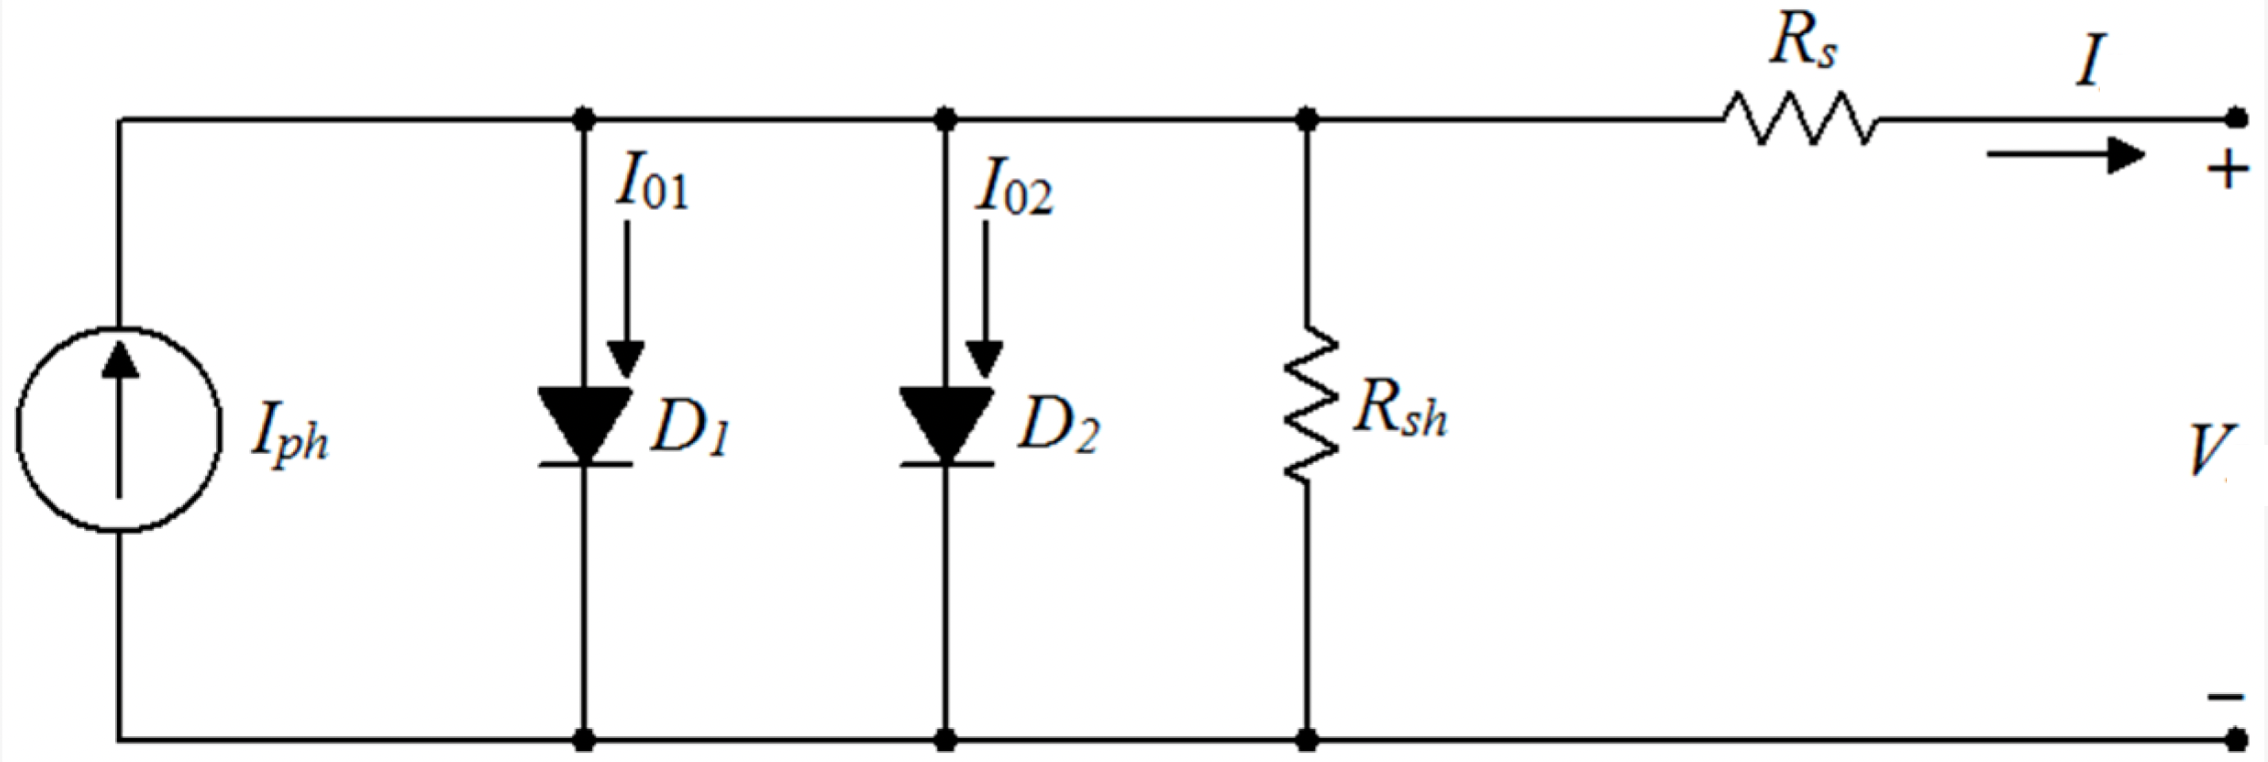
\includegraphics[width=8cm, height=3cm] {sevenp.png}
    \caption{double diodes model \cite{kalogiroubook}}
    \label{fig:my_label}
\end{figure}
\hfill \break
The figure above represents the double-diode electrical equivalent circuit of a photovoltaic (PV) cell, which is a more complex model than the single-diode equivalent circuit. In addition to the four components of the single-diode model - a current source, a shunt resistance, a series resistance, and a diode. The double-diode model includes an additional diode to account for the recombination losses that occur within the PV cell. This more accurate model better represents the behavior of the PN junctions in the PV cell, and is therefore more suitable for analyzing and optimizing the performance of PV cells in practical applications.\\
\hfill \break
The mathematical model becomes:\\
\begin{equation}
I = I_{ph} - I_{s1} \{ exp
 \left[  \frac{q(V+IR_{s})}{n_{1}k_{B}T_{c}} \right] - 1 \} - I_{s2} \{ exp
 \left[  \frac{q(V+IR_{s})}{n_{2}k_{B}T_{c}} \right] - 1 \} - \frac{V+IR_{s}}{R_{sh}}
\end{equation}
\\
Which is an equation with 2 unknowns (I and V) and seven parameters to determinate. These parameters are:

\begin{itemize}
    \item $I_{ph}$: photo-current (A)
    \item $I_{s1}$: first diode reverse saturation current (A)
    \item $I_{s2}$: second diode reverse saturation current (A)
    \item  $n_{1}$: first diode ideality factor
    \item  $n_{2}$ second diode ideality factor
    \item $R_{s}$: series resistance ($\Omega$)
    \item $R_{sh}$: Shunt resistance or the parallel resistance ($\Omega$)
\end{itemize}

\section{Dependency on external and internal parameters}

Several parameters affect, directly and indirectly, the efficiency and the power output of a photovoltaic panel. To improve the performance of the device and to make it more predictable, it is important to understand the relation between the most important characteristics of a photovoltaic panel and the different parameters. Those parameters divide into internal and external ones\cite{texbook6}. 
\subsection{Internal parameters}
Internal parameters, or device-dependent parameters, determine the behavior of the photovoltaic panel and have a significant influence on its performance. These parameters are typically identified using simple electrochemical measurements, such as short-circuit current Isc, open-circuit voltage Voc, maximum power point MPP, the maximum power generated by the photovoltaic panel, and the fill factor (FF).

\subsubsection{Photocurrent}
The photocurrent is produced in PV cells in direct proportion to the intensity of incident radiation and depending on the technical characteristics of the PV panel. Under normal operating conditions, the intensity of solar radiation changes by a few percent, resulting in a change in the amount of photocurrent generated in the cell. It should be noted that the temperature also affects the output of the PV panel and reduces its efficiency. The current $I_{ph}$ for a period of hours, when the sensor is illuminated, is calculated by the following expression:
\begin{equation}
I_{ph} = \frac{G}{G_{n}} 
 \left[ I_{sc} + 	\alpha(T- T_{n}) \right] 
\end{equation}
Where:
\begin{itemize}
    \item G: intensity of solar radiation $(W/m^2)$
    \item $G_{n}$: intensity of solar radiation at standard conditions $(W/m^2)$
    \item $\alpha$: Temperature coefficient of the short circuit current (A/K)
    \item T: cell´s internal temperature (K)
    \item $T_{n}$: cell´s internal temperature in the standard test condition (K)
    \item $I_{sc}$: short circuit current (A)
\end{itemize}

\subsubsection{Internal cell temperature}
The internal cell temperature is the temperature of the PV cell, which is the main factor affecting the efficiency of the photovoltaic panel. The temperature of the PV cell is determined by the temperature of the environment, the intensity of solar radiation, and the heat generated by the PV cell itself. 
\subsubsection{Fill factor}
The fill factor (FF) is another important parameter that characterizes the performance of a photovoltaic panel. It represents the ratio of the maximum power that can be obtained from a solar cell to the product of the open-circuit voltage and short-circuit current. In other words, the fill factor indicates how well a solar cell can convert sunlight into electricity.\\
\\
The fill factor is influenced by various factors, such as the internal resistance of the cell, the quality of the contacts between the cell and the external circuit, and the non-uniformity of the cell material. Typically, the fill factor ranges from 0.5 to 0.8, and higher fill factors indicate better performance of the solar panel.\\
\\
To optimize the performance of a photovoltaic panel, it is important to carefully select the materials and manufacturing processes used in its construction, as well as to take into account factors such as the internal cell temperature and the diode ideality factor. By optimizing these parameters, it is possible to increase the efficiency and performance of a solar panel, making it a more effective and sustainable source of energy.\\
\\
The fill factor (FF) is defined as the ratio of the maximum power output of a solar cell to the product of its open-circuit voltage (Voc) and short-circuit current (Isc), and is expressed mathematically as:
\begin{equation}
FF  = \frac{P_{max}}{Voc \times Isc} 
\end{equation}
Where Pmax is the maximum power output of the cell, and Voc and Isc are the open-circuit voltage and short-circuit current, respectively. 
\subsubsection{Diode ideality factor}
The diode ideality factor is a parameter that compares how much our diode differs from an ideal diode. It describes the level of imperfection in the diode. For an ideal diode, this factor would be equal to 1. This parameter depends on the manufacturing process of the diode and especially on the kind of material used. For instance, the ideality factor of a silicon diode is usually 1.5.

\subsubsection{Diode reverse saturation current}
The diode reverse saturation current is the current that flows through the diode when it is reverse-biased. It has a high impact on the behavior of solar panels. Mainly, it affects the current-voltage characteristic and limits the maximum current in the circuit. It is controlled by temperature. Diode reverse saturation current depends on the quality of solar panels and manufacturing process technology. The mathematical equation to calculate this current is as the following:
\begin{equation}
I_{s} = I_{sn}\left(\frac{T}{T_{n}}\right)^3  exp\left[ \frac{qE_{g}}{nk_{B}} \left( \frac{1}{T_{n}} - \frac{1}{T} \right)\right] 
\end{equation}


Where:
\begin{itemize}
    \item $E_{g}$: band gap energy (eV)
    \item $k_{B}$: Boltzmann constant (J/K)
    \item n:  diode ideality factor
    \item T: cell´s internal absolut temperature (K)
    \item $T_{n}$: cell´s internal temperature in the standard test condition (K)
    \item q: electronic charge (C)
    \item $I_{sn}$: internal diode current in the standard test condition (A) and it's calculated as the following :
    \begin{equation}
I_{sn} = \frac{I_{sc}}{exp\left( \frac{V_{oc}}{nV_{T}} \right)}
\end{equation}
Where:
\begin{itemize}
    \item $I_{sc}$: short circuit current (A)
    \item $V_{oc}$: open circuit voltage (A)
    \item $V_{T}$: thermal voltage and its calculated as the following : 
    \begin{equation}
V_{T} = \frac{k_{B} T}{q}
\end{equation}
\end{itemize}
\end{itemize}

\subsubsection{Series resistance}
Series resistance is situated in series with the diode and it affects the model output but not significantly, especially if the load resistance is large enough  The influence of series resistance is negligible compared to the influence of shunt resistance. Its initialized by the following equation:
\begin{equation}
R_{S} = -\left( \frac{dV}{dI} \right)_{V=V_{oc}}
\end{equation}

\subsubsection{Shunt resistance}
Shunt resistance is situated parallel to the diode so, when there is a voltage applied and the current flows through the diode, it creates a voltage drop. It also affects the model´s output. Lower shunt resistance causes a higher voltage drop and a lower output current of the model. Increased temperature leads to a lower shunt resistance value. Its initialized by the following equation:
\begin{equation}
R_{sh} = -\left( \frac{dV}{dI} \right)_{I=I_{sc}}
\end{equation}

\subsection{external parameters}
The external parameters that affect the performance of a photovoltaic panel could be environmental such as irradiation and temperature and could be physical such as the shadow of an obstacle that interrupts irradiation or decreases temperature.

\subsubsection{Environmental Parameters}
There are different environmental parameters such as irradiation, wind speed, ambient temperature, humidity, and rain that influent the performance of the photovoltaic system. Most of the parameters influence indirectly the system's efficiency by affecting the two most important parameters that have a high impact on the performance of PV systems. The most important parameters are solar irradiation and ambient temperature:

\begin{enumerate}
    \item Irradiation: is a key factor in solar energy conversion and it could be measured using a pyranometer. It is the amount of energy received by a surface per unit of time. This energy is received as electromagnetic radiation from the sun. The amount of energy received by a surface depends on the angle of incidence of the sun's rays, the angle of inclination of the surface, the time of the day, the season of the year, the latitude of the place, the presence of clouds, etc. The amount of energy received by a surface is measured in $W/m^2$. With sufficient solar radiation, photovoltaic cells generate DC voltage and current, which can be used to power electrical equipment.
    \item Ambient temperature: this is an important factor in solar energy conversion and it could be measured easily by a thermometer. Photovoltaic cells operate with ideal efficiency in the range of 20 to 70°C. If the temperature is lower than 20°C, the efficiency decreases slightly. The reason for this is the reduction in mobility of the photovoltaic cells' atoms, which has a direct impact on the energy produced. Conversely, if the temperature is greater than 70°C, the efficiency decreases significantly, as the photovoltaic cells increase their resistance and limit the current flow. In addition to the decrease in efficiency, temperature increases the degradation rate of the photovoltaic panels, so they should be kept at a temperature as low as possible.
\end{enumerate}

\subsubsection{Shadow of Obstacle on PV Panel}

The photovoltaic panels have their potential power affected by the shadow of obstacles. This can result in a decrease or even complete loss of performance for the PV array. Shadows from buildings, trees, or other objects, as well as dust and physical damage to the panels, are examples of obstacles that can cause this reduction. These obstacles can be divided into two categories:
\begin{enumerate}
    \item Short-period shading: a short-term shadowing or temporary shadow. It usually lasts only a few seconds. Short-term shadows can be caused by birds, leaves, or clouds. There are also shadows from passing clouds, that are moving with the clouds.  It is also called a time-dependent obstacle because time can change obstacle behavior.
    \item Long-period shading : or long-time shadow is a long, fixed obstruction and is also called a time-independent obstacle. This type of obstacle is fixed to a certain place and does not change its position over time, and it creates a permanent shadow (for example, buildings, trees, land cover, etc...). 
\end{enumerate}

\section{Generation of measurements database}
An existing database is utilized for the purpose of training the model. The database comprises 21046 samples of location, weather, and power measures gathered over a period of 14 months, from May 2017 to October 2018. These measures were taken at 12 distinct locations situated in the northern hemisphere and consist of 17 features that provide descriptions of the weather, location, and output power of the photovoltaic panels.\\
\\
Let take a look of the first five rows of the data:
\begin{figure}[h!]
    \centering
    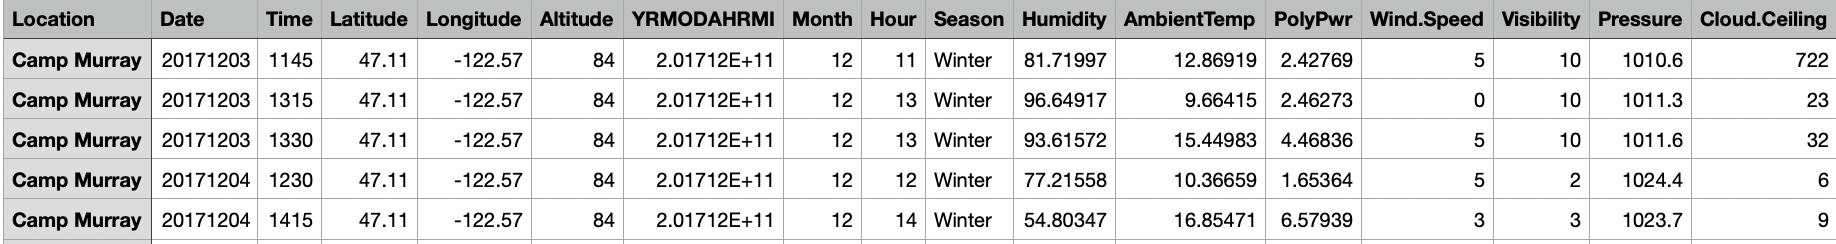
\includegraphics[width=15cm, height=3cm] {rowsdata.png}
    \label{fig:my_label}
\end{figure}
\newpage
\hfill \break
The data can be separated into 3 types or categories: 
\begin{itemize}
    \item Location: are inputs that describe or have relation to the place of this data was measured. It consists of location, latitude, longitude, and altitude inputs.
    \item Date or timing: are inputs that describe or have relation to the position of the panels. It consists of date, time, month, YRMODAHRMI, hour, and season.
    \item Weather: are inputs that describe or have relation to the weather. It consists of humidity, ambient temperature, wind speed, visibility, pressure, and cloud ceiling.
\end{itemize}
\hfill \break
\begin{figure}[h!]
    \centering
    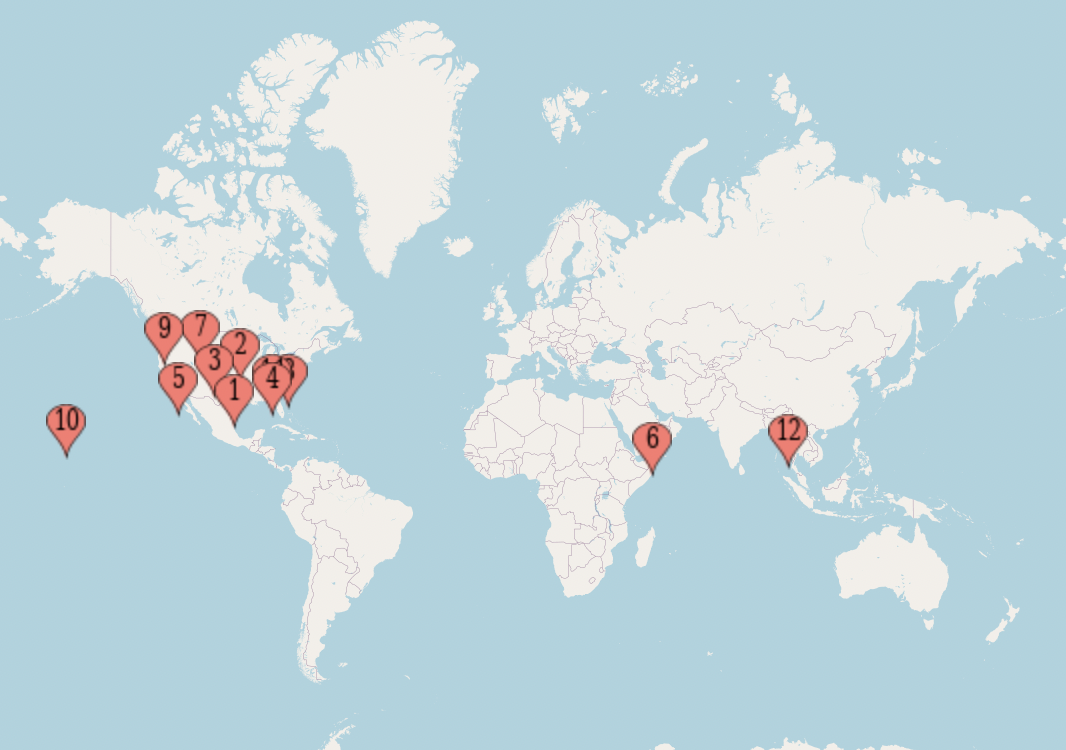
\includegraphics[width=13cm, height=8cm]{map.png}
    \caption{Locations}
    \label{fig:my_label}
\end{figure}
Figure 2.18 represent the different locations that will be use within this project.\\
\newpage
The locations in our data consist of :
\begin{enumerate}
    \item Travis
    \item Peterson
    \item USAFA
    \item Hill Weber
    \item March AFB
    \item JDMT
    \item Malmstrom
    \item Grissom
    \item Camp Murray
    \item Kahului
    \item Offutt
    \item MNANG
\end{enumerate}
In the subsequent chapter, a measurement system is established using an ESP32 model and a variety of sensors, in order to obtain new and realistic data related to the solar panel. This will aid in enhancing the accuracy of the machine-learning model.\\
\chapter{Embedded system}
\noindent\rule{13cm}{1.2pt}\hfill \break
In this chapter, the configuration and programming of an ESP32 model is carried out for the purpose of taking the necessary measurements, formatting them, and storing them in the database. The measurement system plays a crucial role in data acquisition in the project. Given the limited time and resources, the measurement will be added to the existing database to improve the model in the future. The configuration of the ESP32 circuit using a few sensors is the first step. Then, the model is programmed to retrieve values from the sensors. Finally, the obtained data is formatted and stored in the database.
\hfill \break
\noindent\rule{13cm}{1.2pt}

\newpage
\hfill \break
\section{Literature Review of Supporting Techniques} The data acquisition processes described in this chapter are supported by several techniques that have been documented in the literature. These techniques include the use of microcontrollers such as the ESP32 for data collection and processing, and the use of breadboards for connecting sensors and other hardware components.\\
\\
Microcontrollers have been widely used for data acquisition due to their ability to collect and process data from various sensors. Some articles discusses how microcontrollers can be programmed to perform specific tasks such as filtering and analyzing data. This makes them a versatile tool for data acquisition in various applications\cite{Smith2018}.\\
\\
Breadboards are also commonly used for connecting hardware components in data acquisition systems. Some books provides step-by-step instructions on how to use a breadboard to connect various components such as sensors and microcontrollers. She also provides tips on how to troubleshoot common issues that may arise when using a breadboard\cite{Doe2017}.\\
\\
In conclusion, the literature reviewed in this section provides valuable support for the data acquisition processes described in this chapter. Further research can uncover additional techniques that may be applicable to specific applications.
\section{Configuration}
To successfully complete the data acquisition processes described in this report, several pieces of hardware must be configured to take the necessary measurements. This section describes the hardware requirements for achieving this step and includes images of the devices.

\subsection{Hardware requirements}
An ESP32 microcontroller is utilized and connected to a breadboard for this project. Additional sensors are also connected to the breadboard.\newpage
\begin{itemize}
    \item ESP32 : a Wi-Fi-enabled 32-bit ARM Cortex-M0 + microcontroller that features a dual-core ARM® Cortex™-M0 processor operating at 80 MHz. It has 512 KB flash memory and is integrated with 2 MB RAM. It also has a low-power Bluetooth Low Energy and a 128 MB SD card slot. The ESP32 is manufactured with a 180 nm CMOS process and is an ideal general-purpose microcontroller with a wide range of applications. It's presented in the following figure :
    \begin{figure}[h!]
  \centering
    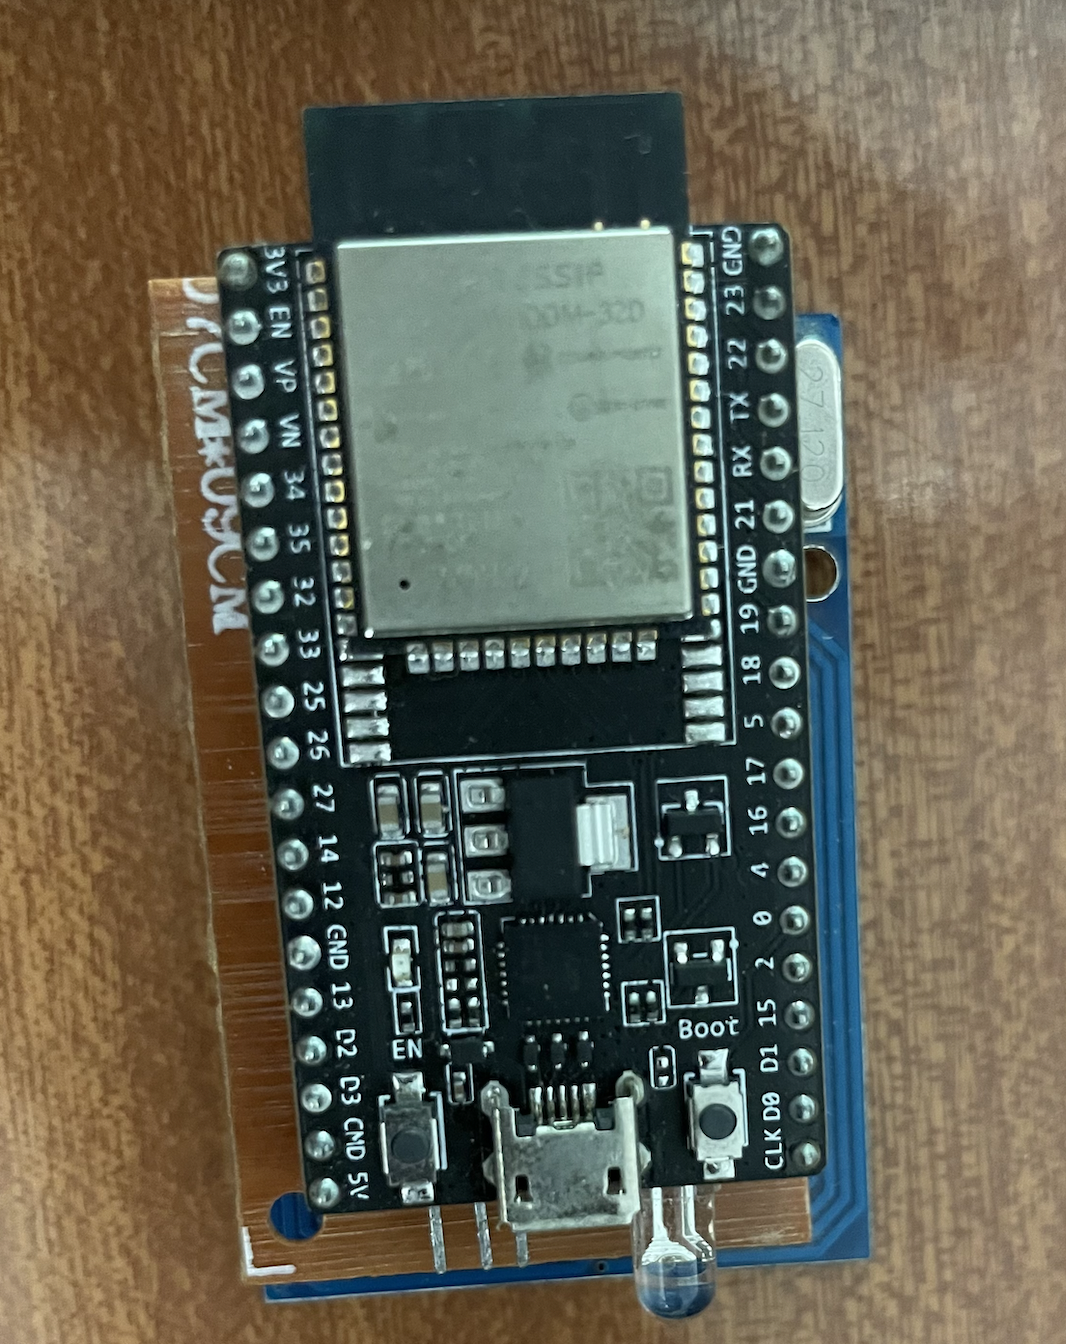
\includegraphics[width=5cm, height=8cm, angle=90] {esp32.png}
    \caption{ESP32 model}
    \label{fig:my_label}
\end{figure}
    \item Breadboard : a rectangular plastic board with tiny holes arranged in rows and columns. Small pieces of metal wire called breadboard straps can be inserted to connect wires running to components mounted on the breadboard such as sensors. It's presented in the following figure :
    \begin{figure}[h!]
    \centering
    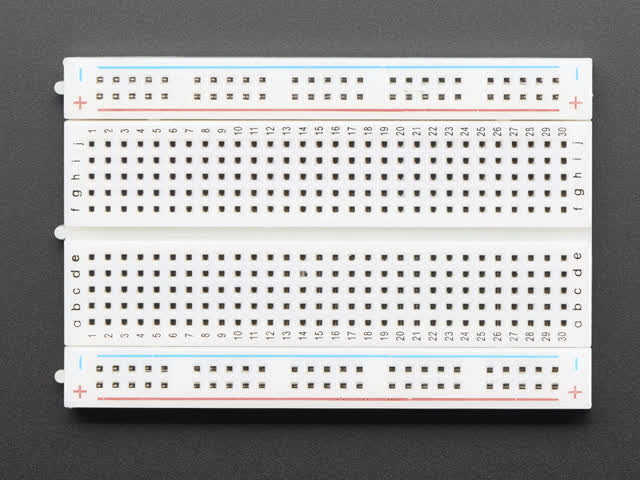
\includegraphics[width=8cm, height=5cm] {Breadboard.jpeg}
    \caption{Breadboard}
    \label{fig:my_label}
    \end{figure}\newpage
    \item Quectel L86 GPS Module : is an embedded patch antenna GPS receiver module that comes with a built-in antenna, MCU with U-Blox GPS receiver, and tracking telemetry circuit. It can work with a smart device through a BlueTooth connection, making it convenient for collecting data from the solar system. It's presented in the following figure :
    \begin{figure}[h!]
    \centering
    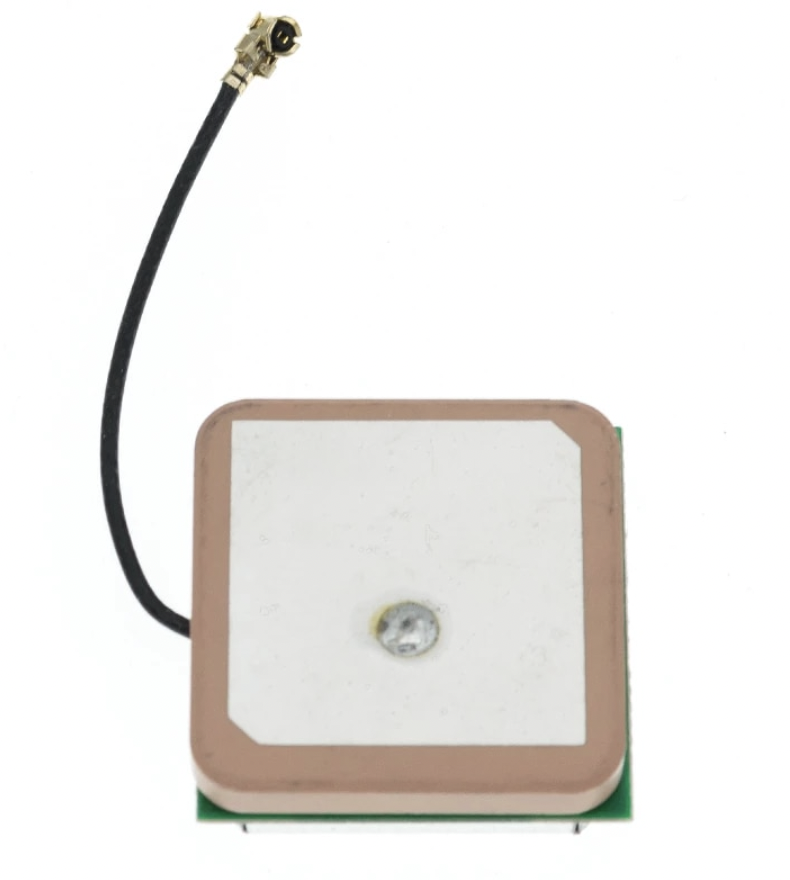
\includegraphics[width=8cm, height=5cm] {gps.png}
    \caption{Quectel L86 GPS}
    \label{fig:my_label}
    \end{figure}\hfill \break
    \item AM2301B : a temperature and humidity sensor designed for environment measurement. It is a self-integrated circuit, with low power consumption, low cost, high performance, and easy to interface. It can be used to measure solar irradiation, indoor and outdoor temperature, and humidity. It's presented in the following figure :
    \begin{figure}[h!]
    \centering
    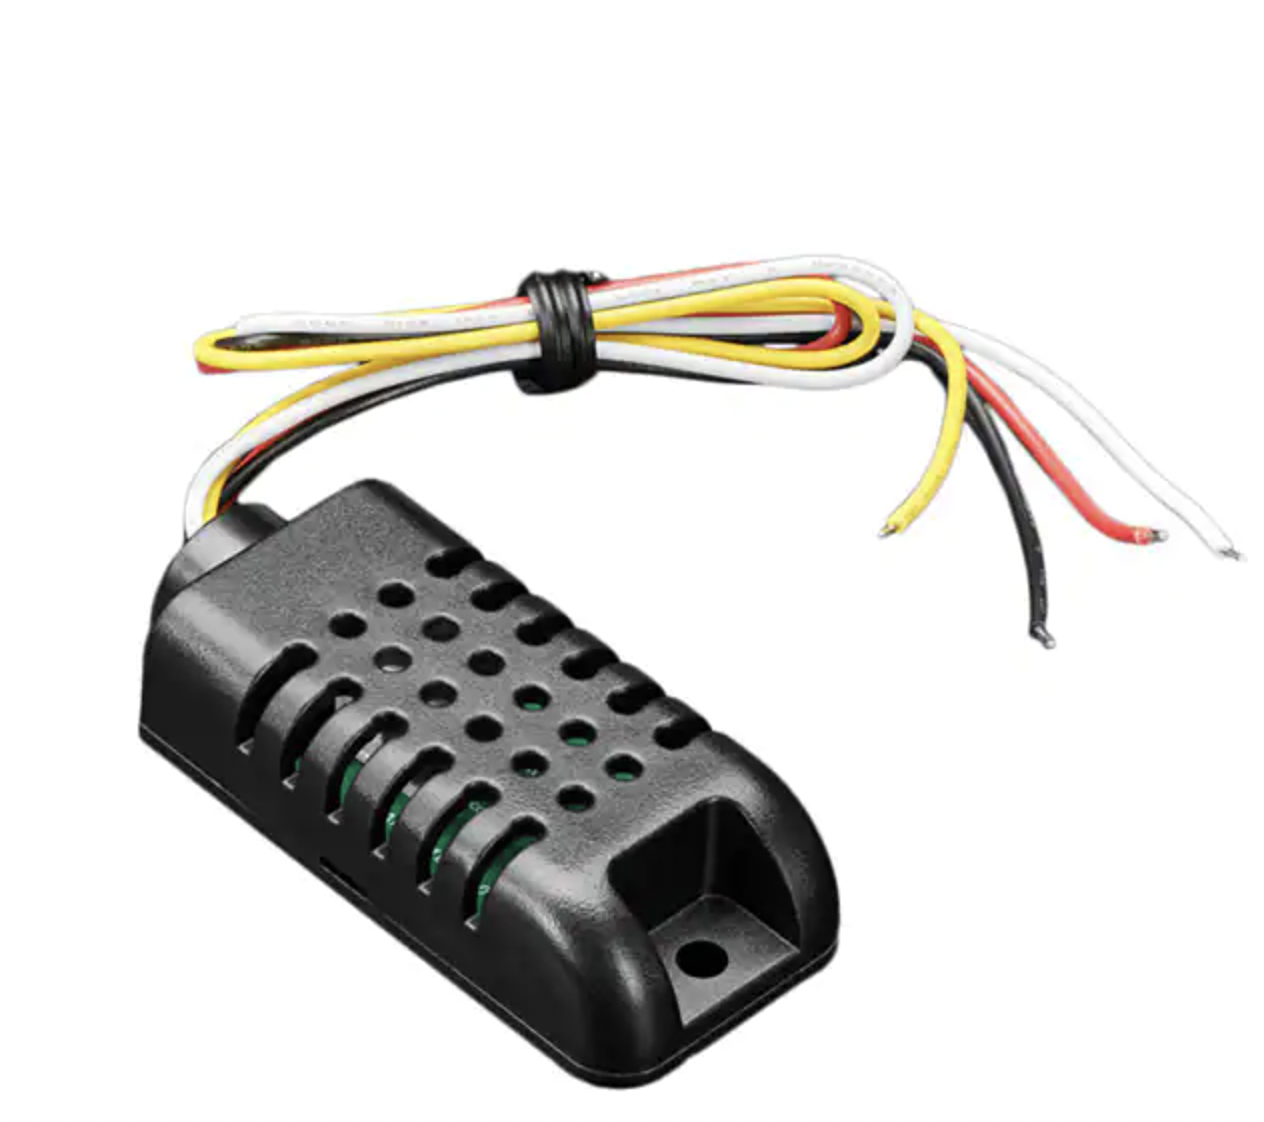
\includegraphics[width=8cm, height=5cm] {temper.png}
    \caption{AM2301B}
    \label{fig:my_label}
    \end{figure}\hfill \break \\
    
    \item  BGT-FS1 : a wind speed sensor that uses a hot wire anemometer system. The air velocity is measured with a probe and the total static pressure is with a Pitot tube. By the end, the wind speed is calculated by the pressure difference between the two tubes. It's presented in the following figure :
    \begin{figure}[h!]
  \centering
    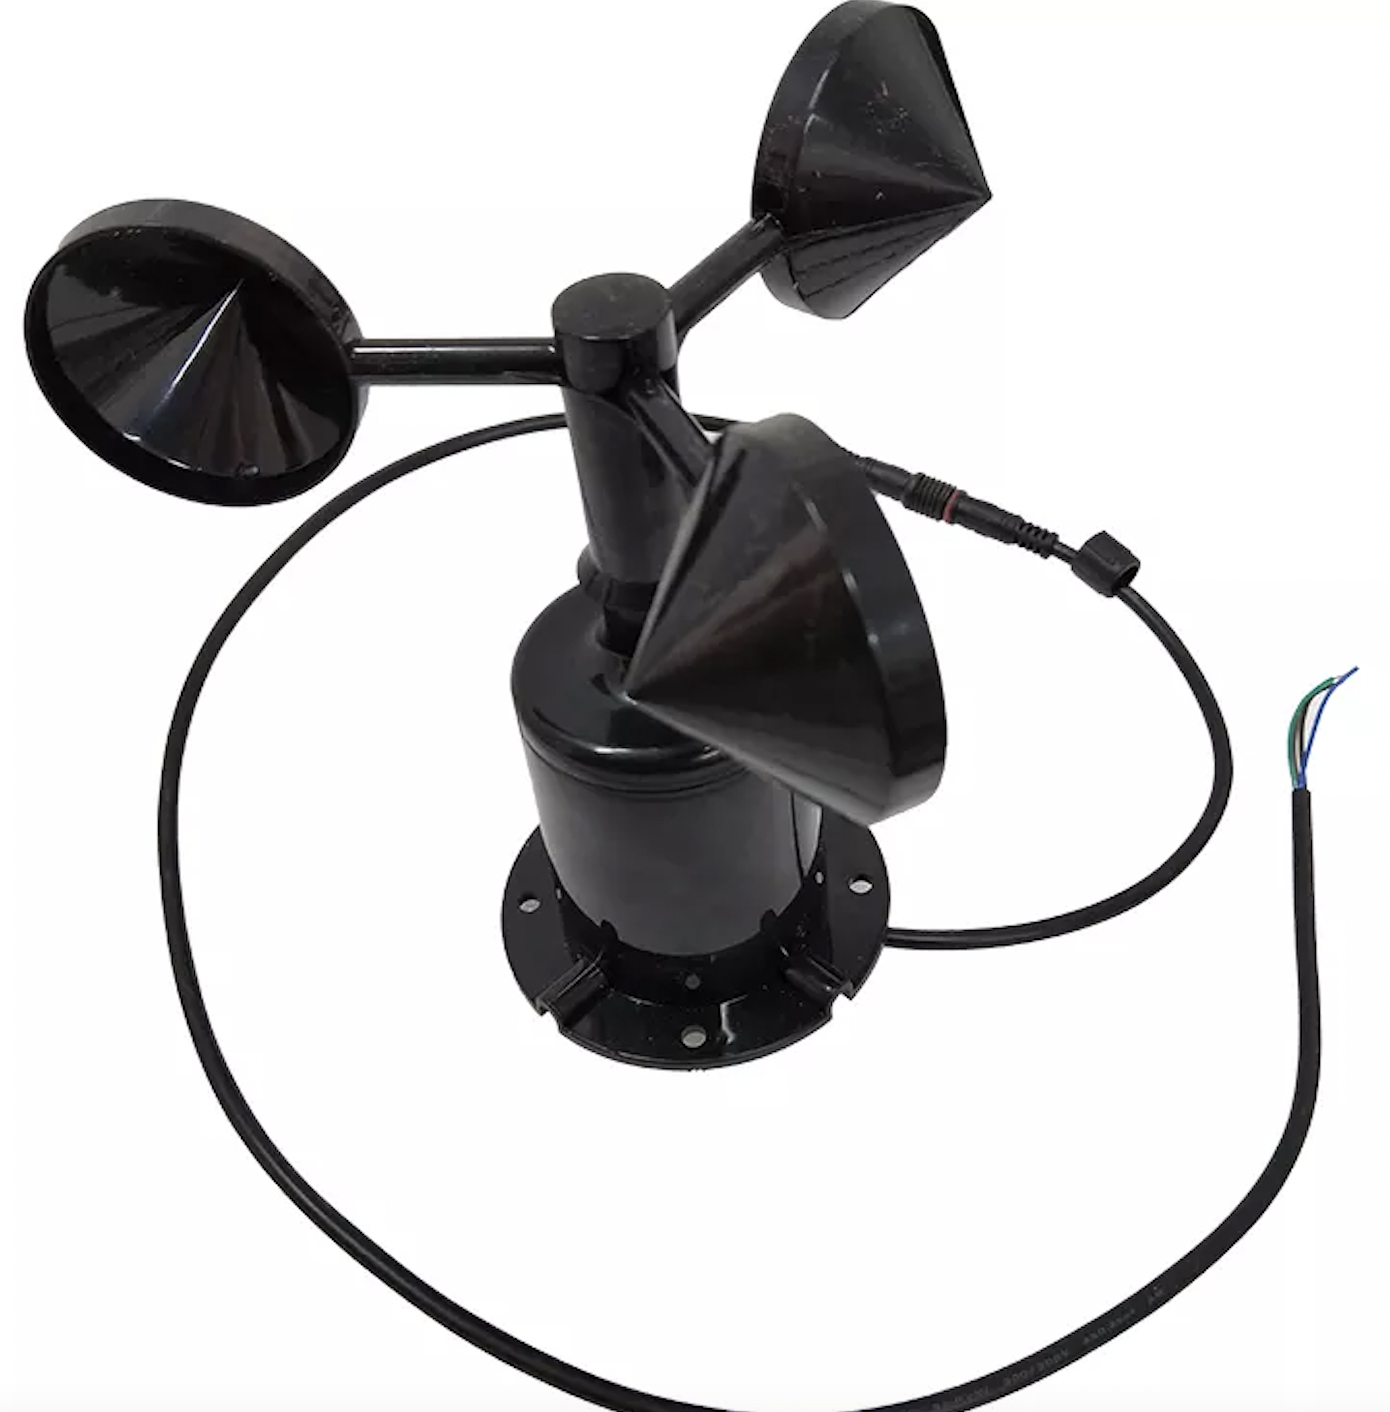
\includegraphics[width=8cm, height=5cm] {BGT-FS1.png}
    \caption{BGT-FS1}
    \label{fig:my_label}
    \end{figure}\hfill \break
\end{itemize}
The process begins by connecting the ESP32 to the breadboard, which is then linked to the power source. The Quectel L86 GPS is used to obtain the three location parameters: latitude, longitude, and altitude. The AM2301B sensor is used to acquire air humidity and ambient temperature, which can be converted to relative humidity. The BGT-FS1 is employed to measure wind speed and pressure. Since it is challenging to obtain values for visibility and cloud ceiling, these parameters will be retrieved online. The other sensors are also connected to the breadboard.
\subsection{Software requirements}
There are numerous websites that provide the values of visibility and cloud ceiling, as well as other parameters, using the location parameters. An example of such websites will be demonstrated.
\newpage
\begin{figure}[h!]
  \centering
    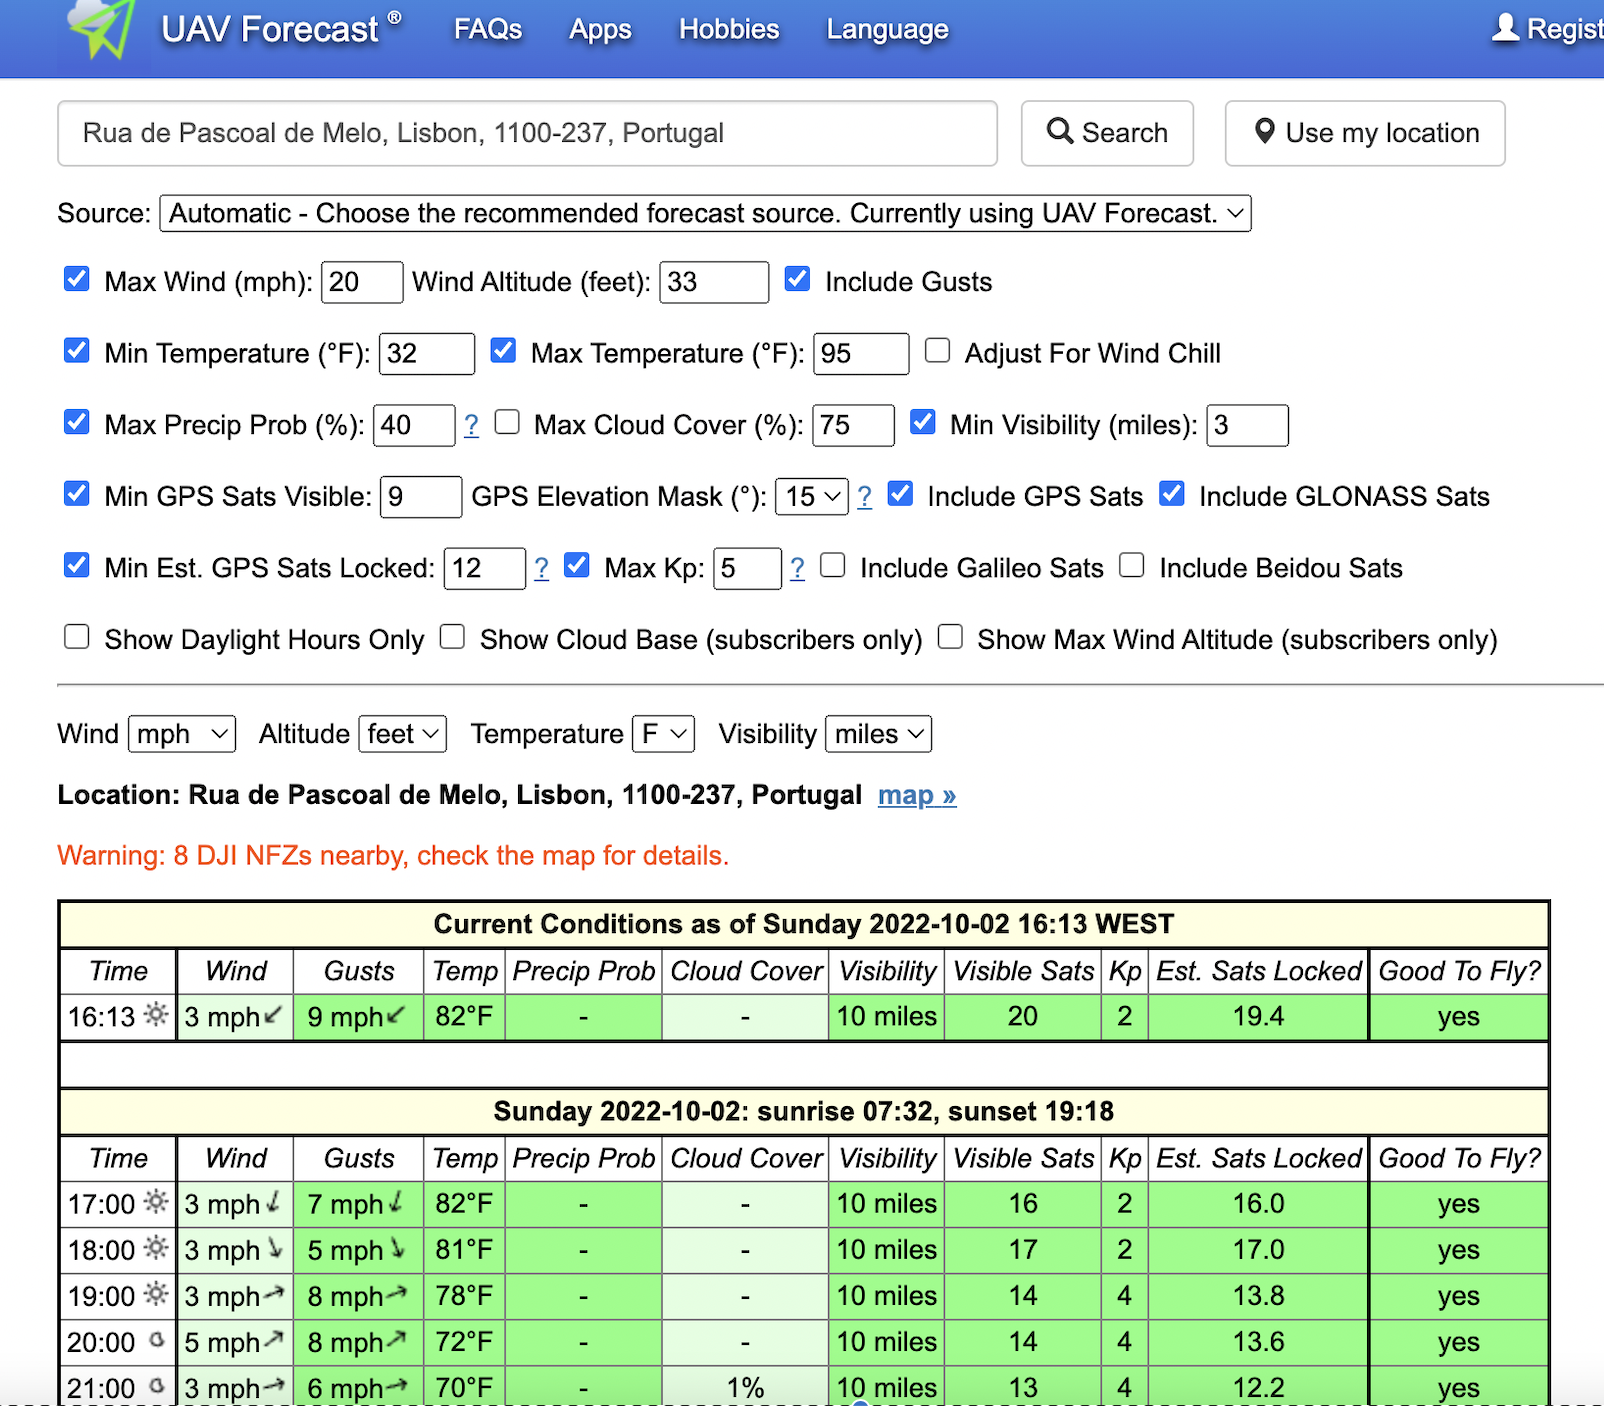
\includegraphics[width=12cm, height=7cm] {website.png}
    \caption{UAV forecast\cite{uav}}
    \label{fig:my_label}
\end{figure}
\hfill \break 
The UAV forecast website is represented in Figure 3.6. It provides the weather forecast and its parameter values every minute, including ambient temperature, pressure, humidity, wind speed, visibility, and cloud ceiling. These weather values can be obtained by using the website.
\hfill \break \\
Taking the measurements using ESP32 sensors will be explained in the programming section.

\section{Programming}
\subsection{Software requirements}
ESP32 can be programmed in different languages and different programming environments. Some of the most common are:

\begin{itemize}
    \item Arduino IDE: written in C++, using cross-platform libraries. IDE is available on Windows, Mac, and Linux.
    \item CircuitPython: MIT-licensed programming language specifically designed for microcontrollers. Programming is done directly on the microcontroller using its pins.
    \item Espressif IDF (IoT Development Framework): Espressif IoT IDE. It has all the features of the Arduino IDE, plus a wide range of optimizations, for use in industrial environments.
    \item LUA : is a powerful programming language often used in IoT development. CooCox IDE offers  native support for LUA.
    \item CooCox IDE: written in C, for advanced users.
    \item MicroPython: open-source, community-driven programming language, designed for microcontrollers.
    \item Net Micro Framework (MNF): It is a software platform designed for the firmware development of microcontrollers.
\end{itemize}

\subsection{Quectel L86 GPS Module Programming}

\subsubsection{Code Explanation}

The necessary libraries are first imported. The machine library is imported for the use of UART1, the time library for the sleep function, the pyb library for the LED function, and the math library for the floor function. Then, UART1 is initialized\cite{q}. After that, three functions are defined:
\begin{itemize}
    \item convert\_to\_degrees: This function takes the latitude and longitude in degrees, minutes, and seconds as input and converts them to decimal degrees. The decimal degrees are calculated by dividing the degrees by 100 and then adding the minutes and seconds to it. The minutes and seconds are calculated by dividing the minutes and seconds by 60 and then adding them to the degrees. The decimal degrees are then rounded off to 4 decimal places.
    \item checksum: This function takes the GPS data as input and calculates the checksum. The checksum is calculated by XORing all the characters in the GPS data. The checksum is then returned.
    \item get\_gps\_data: This function reads the GPS data from the UART1 and then checks if the data is valid. If the data is valid, the latitude and longitude are extracted from the data and converted to decimal degrees. The time, number of satellites, altitude, and checksum are also extracted from the data. The checksum is then calculated and compared with the checksum extracted from the data. If the checksums match, the latitude, longitude, time, number of satellites, and altitude are printed. If the checksums do not match, an error message is printed. The latitude and longitude are then returned.
\end{itemize}

\begin{algorithm}
\caption{GPS }
\begin{algorithmic}[1]
\Procedure{convert\_to\_degrees}{$raw\_value$}
\State $decimal\_value = raw\_value/100.00$
\State $degrees = int(decimal\_value)$
\State $mm\_mmmm = (decimal\_value - int(decimal\_value))/0.6$
\State $position = degrees + mm\_mmmm$
\State %(position)$
\State \Return $ position$ 
\EndProcedure
\\
\Procedure{checksum}{$sentence$}
\State $checksum = 0$
\For{$c$ in $sentence$}
\State $checksum ^= c$
\EndFor
\State \Return $checksum$
\EndProcedure
\\
\Procedure{get\_gps\_data}{}
\State $data = uart.readline()$
\If{$data$ is not None}
\State $data = data.decode('utf-8')$
\If{$data[0:6]$ == 'GPGGA'}
\State $sdata = data.split(",")$
\If{$sdata[2]$ == ''}
\State $lat = 0.0$
\State $lon = 0.0$
\Else
\State $lat = float(convert\_to\_degrees(float(sdata[2])))$
\State $lon = float(convert\_to\_degrees(float(sdata[4])))$
\EndIf
\State \textbf{print}("Latitude: ", lat)
\State \textbf{print}("Longitude: ", lon)
\State \textbf{print}("Time: ", sdata[1])
\State \textbf{print}("Satellites: ", sdata[7])
\State \textbf{print}("Altitude: ", sdata[9])
\State \textbf{print}("Checksum: ", sdata[15])
\State \textbf{print}("Checksum calculated: ", checksum(data[1:-4].encode()))
\State \textbf{print}("
")
\State \Return $lat, lon$
\EndIf
\Else
\State \Return 0.0, 0.0
\EndIf
\EndProcedure
\\
\While{True}
\State get\_gps\_data()
\State time.sleep(1)
\EndWhile
\end{algorithmic}
\end{algorithm}


\subsubsection{Connection with ESP32}
To implement the GPS module with ESP32, the following connections are made:
The GPS module is powered using the 3V3 pin of the ESP32. The GND pin of the GPS module is connected to the GND pin of the ESP32. The TX pin of the GPS module is connected to the RX pin of the ESP32 and the RX pin of the GPS module is connected to the TX pin of the ESP32. 


\subsection{AM2301B Module Programming}
\subsubsection{Code Explanation}

The code to implement the AM2301B module with ESP32 using micropython is pretty straightforward. It takes to initialize the DHT11 sensor and then call the measure() function to get the temperature and humidity values. The measure() function will return the temperature and humidity values in Celsius and percentage respectively\cite{am0}.

\begin{algorithm}
\caption{AM2301B}
\begin{algorithmic}[1]
\Procedure{AM2301B}{$\textbf{dht}$}
\State $dht.measure()$
\State $\textbf{print(dht.temperature())}$
\State $\textbf{print(dht.humidity())}$
\State $time.sleep(2)$
\EndProcedure
\end{algorithmic}
\end{algorithm}

\subsubsection{Connection with ESP32}
To implement the AM2301B module with ESP32, the following connections are required:
\begin{itemize}
    \item The VCC pin of the AM2301B module is connected to the 3.3V pin of the ESP32. 
    \item The GND pin of the AM2301B module is connected to the GND pin of the ESP32.
    \item The DATA pin of the AM2301B module is connected to the GPIO4 pin of the ESP32.
\end{itemize}

\subsection{BGT-FS1}
\subsubsection{Code Explanation}

The code to implement the BGT-FS1 module with ESP32 using micropython is pretty straightforward. The wind speed is calculated by dividing the number of rotations per second by $2\pi$r. 


\begin{algorithm}
\caption{BGT-FS1}
\begin{algorithmic}[1]
\Procedure{rotation}{$pin$}
\State $rotations \gets rotations + 1$
\EndProcedure
\State $sensor \gets machine.Pin(32, machine.Pin.IN)$
\State $interval \gets 1$
\State $rpm \gets 0$
\State $rotations \gets 0$
\State $sensor.irq(trigger=machine.Pin.IRQ_RISING, handler=rotation)$
\While{True}
\State $rpm \gets rotations \times 60 / interval$
\State \textbf{print}($rpm/2\pi r$)
\State $rotations \gets 0$
\State \textbf{time.sleep}($interval$)
\EndWhile
\end{algorithmic}
\end{algorithm}

\subsubsection{Connection with ESP32}
In order to implement the BGT-FS1 module with ESP32, the following connections are required:
\begin{itemize}
    \item BGT-FS1 module pin 1 to ESP32 pin 32
    \item BGT-FS1 module pin 2 to ESP32 pin 3.3V
    \item BGT-FS1 module pin 3 to ESP32 pin GND
\end{itemize}

\section{Data formatting and storage}

The data collected for this study is stored in a comma-separated values (CSV) file. CSV is a format commonly used for storing and exporting data in plain text, and can be created in any program that allows data to be saved in this format.\hfill \break 
\\
The data consists of 17 columns, each with a specific format and meaning. These columns are:

\begin{itemize}
    \item \textbf{Location}: The location of the photovoltaic panel, stored as a string.
    \item \textbf{Date}: The date of the data, stored as an integer in the format YYYYMMDD.
    \item \textbf{Time}: The time of the data, stored as an integer in the format HHMM.
    \item \textbf{Latitude}: The latitude of the photovoltaic panel, stored as a floating-point number.
    \item \textbf{Longitude}: The longitude of the photovoltaic panel, stored as a floating-point number.
    \item \textbf{Altitude}: The altitude of the photovoltaic panel, stored as a floating-point number.
    \item \textbf{YRMODAHRMI}: The date and time of the data, stored as an integer in the format YYYYMMDDHHMM.
    \item \textbf{Month}: The month of the data, stored as an integer.
    \item \textbf{Hour}: The hour of the data, stored as an integer.
    \item \textbf{Season}: The season of the data, stored as a string.
    \item \textbf{Humidity}: The relative humidity of the data, stored as a floating-point number.
    \item \textbf{AmbientTemp}: The ambient temperature of the data, stored as a floating-point number.
    \item \textbf{Wind.Speed}: The wind speed of the data, stored as a floating-point number.
    \item \textbf{Visibility}: The visibility of the data, stored as a floating-point number.
    \item \textbf{Pressure}: The atmospheric pressure of the data, stored as a floating-point number.
    \item \textbf{Cloud.Ceiling}: The height of the cloud ceiling, stored as a floating-point number.
\end{itemize}
The purpose of the data collection is to analyze the relationship between the power output of the photovoltaic panel and the other 16 columns. In the following chapter, this relationship will be analyzed, and a machine learning algorithm will be developed to predict the power output of the photovoltaic panel based on the other 16 columns.

\chapter{Machine learning system}
\noindent\rule{13cm}{1.2pt}\hfill \break
This chapter will present a description of the machine learning system that was developed for predicting the power of a photovoltaic panel. The system was developed using the Python programming language and the scikit-learn library. The development of the machine learning system involved the following steps:
\begin{itemize}
    \item Data exploration
    \item Data preparation
    \item Model selection
    \item Model evaluation
    \item Model deployment
\end{itemize}
\hfill \break
\noindent\rule{13cm}{1.2pt}

\newpage
\hfill \break
\section{Similar Work Review}
The Medium post "Predicting solar power output using machine learning techniques", covers data exploration, data pre-processing, and feature engineering. The authors utilize machine learning techniques to predict solar power output from 12 northern hemisphere locations. The data exploration step involves analyzing the characteristics of the data that will be used to train and evaluate the model, and identifying any potential challenges or issues that may affect the model’s performance. Data pre-processing includes finding and handling outliers in the dataset and data encoding. Feature engineering is used to develop three models, including Random Forest, Light Gradient Boosting Machine, Deep Neural Network, and a stacked ensemble that are compared using the R-squared metric.\\
\\
Overall, the author's research concludes that the Random Forest model was the most accurate in predicting power output, and its performance is comparable to those that include measurements of irradiance. The inclusion of location and weather data without information about irradiance saves time, effort, and cost in data collection. Additionally, the document includes details on state-of-the-art photovoltaic technology and lays out a roadmap for future research and development in the field of photovoltaic panels.
\section{Data Exploration}
Data exploration is an important step in the process of developing a machine learning model. It involves analyzing the characteristics of the data that will be used to train and evaluate the model, and identifying any potential challenges or issues that may affect the model's performance. This process typically includes a combination of summary statistics, visualizations, and other analysis techniques to help understand the nature and structure of the data. By thoroughly exploring the data, researchers and data scientists can gain insights into the data that can guide the development of the machine learning model and help to ensure that it performs well on real-world data.
\begin{figure}[h!]
  \centering
    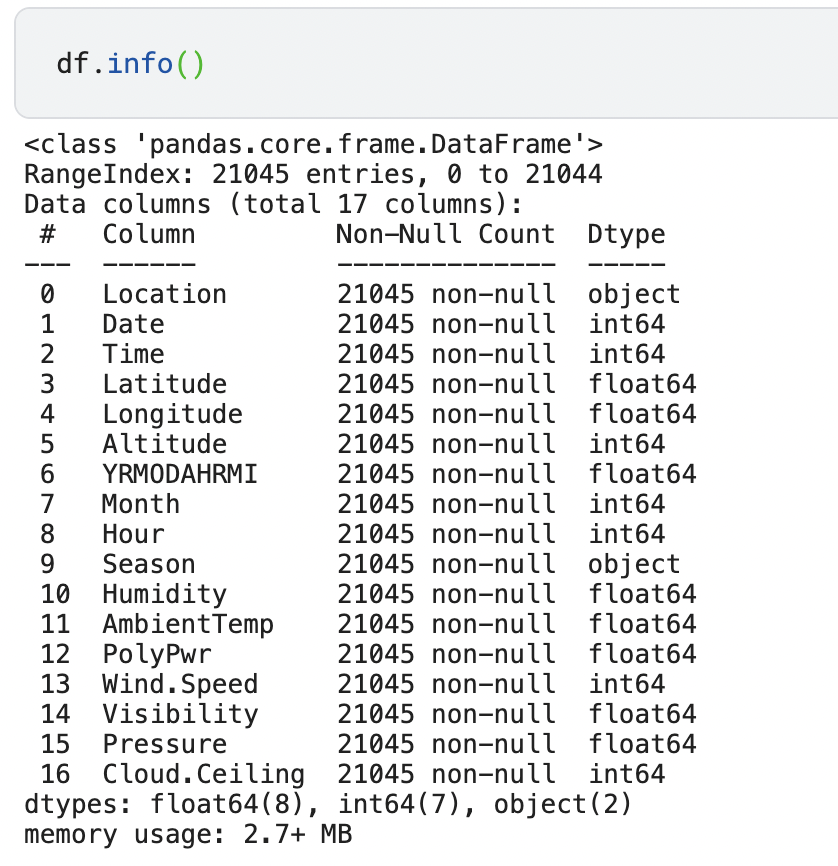
\includegraphics[width=8cm, height=8cm] {info.png}
    \caption{DataFrame.info output}
    \label{fig:my_label}
\end{figure}\\
\\
Figure 4.1 displays the output of data.info() for a dataset that contains 21,045 rows of environmental data. The dataset comprises 17 columns, including location, date, time, latitude, longitude, altitude, and various environmental measurements. The data.info() method provides an overview of the dataset's structure, including the number of non-null values for each column, the data type of each column, and the memory usage of the dataset.\\
\\
As depicted in Figure 4.1, all columns in the dataset have 21,045 non-null values, indicating the absence of missing values. Most columns have a data type of either float64 or int64, suggesting that they contain numerical data. Meanwhile, the 'Location' and 'Season' columns are represented by object data types, which contain categorical data. Furthermore, the output provides information on the amount of memory consumed by the dataset, which is essential for optimizing performance when working with larger datasets.
\subsection{Mean, Standard Deviation and Quartiles}
Mean, standard deviation and quartiles are metric statistics that describe the distribution of the data. 
\subsubsection{Mean}

The mean is the average value of a set of data and is calculated by adding all the values together and then dividing the sum by the total number of values. This provides a summary of the central tendency of the data. The mean can be calculated using the following equation:
\begin{equation}
    \bar{x} = \frac{1}{n}\sum_{i=1}^{n}x_i
\end{equation}


\subsubsection{Standard Deviation}

The standard deviation (SD) is a measure of the dispersion of a set of values from its mean. It's calculated by finding the square root of the variance, which is the average of the squared differences of each value from the mean. The formula for calculating the standard deviation is:
\begin{equation}
    \sigma = \sqrt{\frac{\sum_{i=1}^{n}(x_i - \mu)^2}{n}}
\end{equation}
\subsubsection{Quartiles}
The quartiles are the 25th, 50th, and 75th percentiles of the data. The 25th percentile is the value below which 25\% of the data lies. The 50th percentile is the value below which 50\% of the data lies. The 75th percentile is the value below which 75\% of the data lies. The 50th percentile is the median of the data. \hfill \break 
The Interquartile Range (IQR) is the difference between the 75th and 25th percentiles. It's a measure of the spread of the data. after calculating the quartiles and the IQR, the outliers could be found using the following formula:
\begin{itemize}
    \item lower bound = Q1 - 1.5 \times IQR
    \item upper bound = Q3 + 1.5 \times IQR
\end{itemize}
The values that are below the lower bound or above the upper bound are outliers.\hfill \break 
\\
The mean, standard deviation, and quartiles can be obtained by using the describe function in pandas. A screenshot of the output of the describe() function is shown in Figure 4.2.
\begin{figure}[h!]
  \centering
    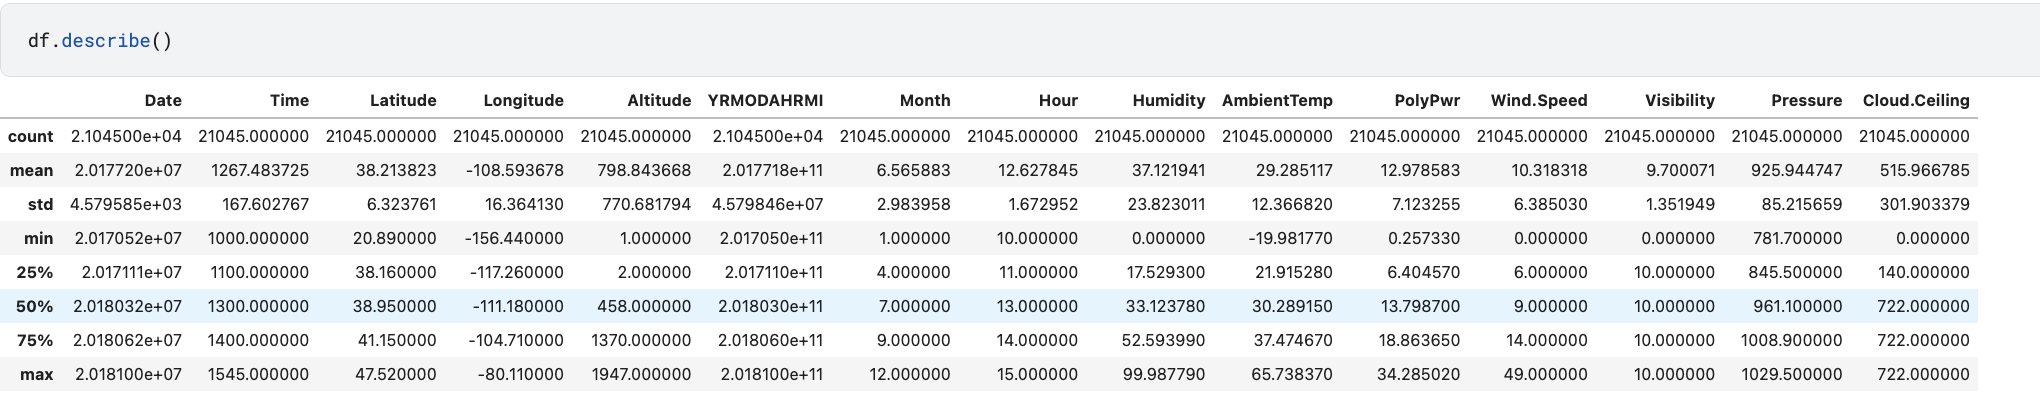
\includegraphics[width=14cm, height=4cm] {describe.png}
    \caption{describe output}
    \label{fig:my_label}
\end{figure}\hfill \break 
\\
Figure 4.2 presents the output of data.describe(), which provides statistical summaries for each column in the dataset. The Date column ranges from 20170520 to 20181001, with a mean of 20177201. The Time column ranges from 1000 to 1545, with a mean of 1267. The Latitude column ranges from 20.89 to 47.52, with a mean of 38.21 and a standard deviation of 6.32. The Longitude column ranges from -156.44 to -80.11, with a mean of -108.59 and a standard deviation of 16.36. The Altitude column ranges from 1 to 1947, with a mean of 798.84 and a standard deviation of 770.68. The YRMODAHRMI column ranges from 201705010000 to 2018100100, with a mean of 2017718123343. The Month column ranges from 1 to 12. The Hour column ranges from 10 to 15. The Humidity column ranges from 0 to 99.99, with a mean of 37.12 and a standard deviation of 23.82. The AmbientTemp column ranges from -19.98 to 65.74°C, with a mean of 29.29 and a standard deviation of 12.37. The PolyPwr column ranges from 0.26 to 34.29, with a mean of 12.98 and a standard deviation of 7.12. The Wind.Speed column ranges from 0 to 49 km/h, with a mean of 10.32 and a standard deviation of 6.39. The Visibility column ranges from 0 to 10, with a mean of 9.70 and a standard deviation of 1.35. The Pressure column ranges from 781.7 to 845.5, with a mean of 925.94 and a standard deviation of 85.22. The Cloud.Ceiling column ranges from 0 to 722, with a mean of 515.97 and a standard deviation of 301.90. The summary statistics presented in Figure 1 provide insights into the range, distribution, and variability of the data in the dataset.
\newpage
\subsection{Data Distribution}
Data distribution is a crucial aspect in understanding the characteristics of a dataset. It provides insights into how the data is spread across different values and helps to identify any patterns or anomalies. The normal distribution, also known as the Gaussian distribution, is the most common and widely studied distribution. In a normal distribution, the data is symmetrically distributed around the mean, median, and mode, and the majority of the data lies within one standard deviation of the mean.\\
\\
However, not all data follow a normal distribution. A skewed distribution is one in which the data is not evenly distributed and has a long tail on one side. A right-skewed distribution has a long tail on the right side, which means that there are a few extreme values towards the right, and the majority of the data is towards the left. In contrast, a left-skewed distribution has a long tail on the left side, indicating that the majority of the data is towards the right and a few extreme values towards the left.\\
\\
In addition to normal and skewed distributions, bimodal data can also be observed. A bimodal distribution is characterized by two peaks, indicating that the data has two modes and two distinct groups of data. For instance, when analyzing students' test scores, researchers may observe two distinct groups - one group of students who performed well and another group who did not perform well.\\
\\
To determine the distribution of data, various statistical techniques and tools can be used. One such tool is the hist function in pandas, which can be used to create a histogram of the data. The histogram helps to visualize the distribution of data and identify any patterns or anomalies that may be present. In the code snippet above, the output of the hist() function for each column is shown in the figures, which helps to analyze the data distribution of each column. 
\begin{figure}
    \centering
    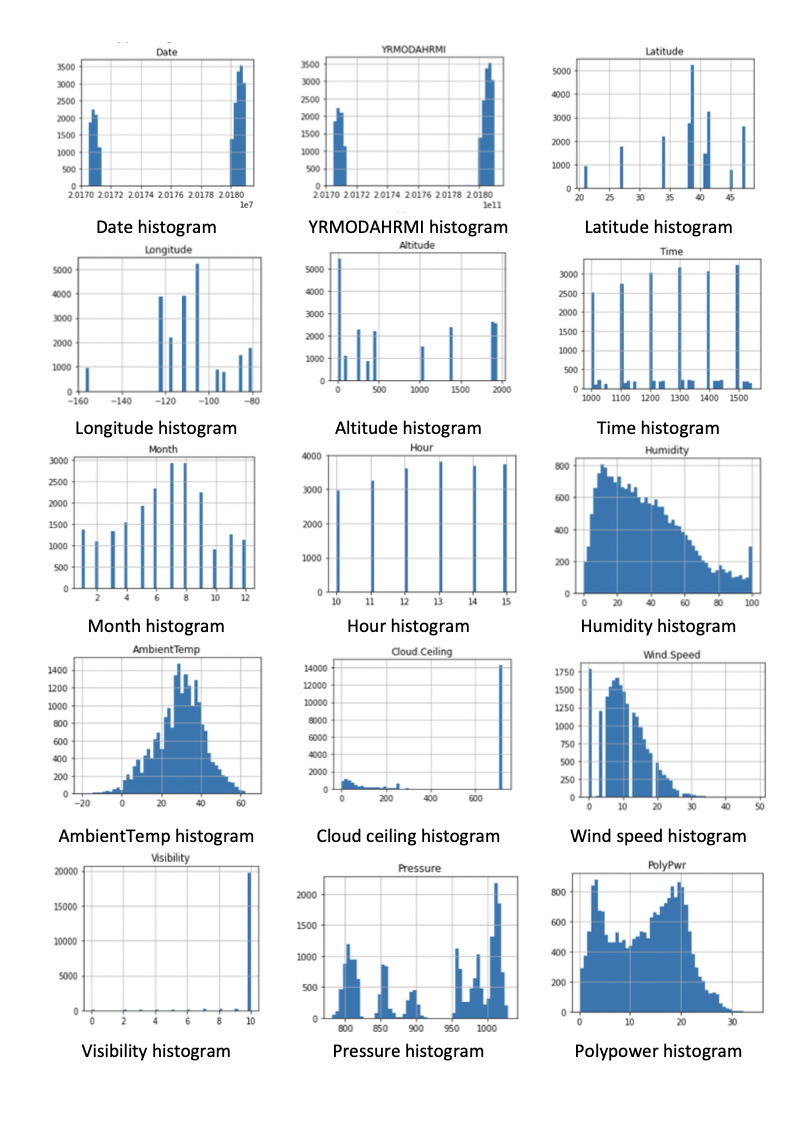
\includegraphics[width=12cm, height=18cm]{123.png}
    \caption{Features Histograms}
\end{figure}\newpage \hfill \break 
\\
Based on the histograms displayed above, it has been observed that the date and YRMODAHRMI features share identical data. This finding suggests a high degree of correlation between the two features and possible redundancy in the information provided. Further analysis revealed that the YRMODAHRMI feature does not offer any additional information beyond the date feature. Consequently, it is recommended that this feature be removed from the dataset, as doing so could simplify the dataset, reduce the feature space's dimensionality, and potentially enhance the machine learning algorithm's performance. Furthermore, removing this feature could aid in reducing model complexity and improving interpretability by eliminating any potential multicollinearity between the features.

\subsection{Correlation between the columns}

the correlation is a statistical measure that indicates the extent to which two or more variables fluctuate together. This means that when one variable is above its mean, the other is likely to be above its mean as well. When computing correlation, it is important to remember that correlation does not imply causation. Correlation measures only the extent of the linear relationship between two variables. It tells us nothing about whether and how strongly the variables are related in some other way. If the correlation is negative, it means that the two variables are inversely related. If one variable increases, the other decreases. If one variable decreases, the other increases. But if the correlation is positive, it means that the two variables are directly related. If one variable increases, the other increases. If one variable decreases, the other also decreases. However, the correlation between Longitude and other features is found to be very weak. As a result, it has been decided to drop the Longitude variable.
If the correlation is zero, it means that the two variables are not related. Figure 4.3 shows the correlation between the columns of our data.

\begin{figure}[h!]
  \centering
    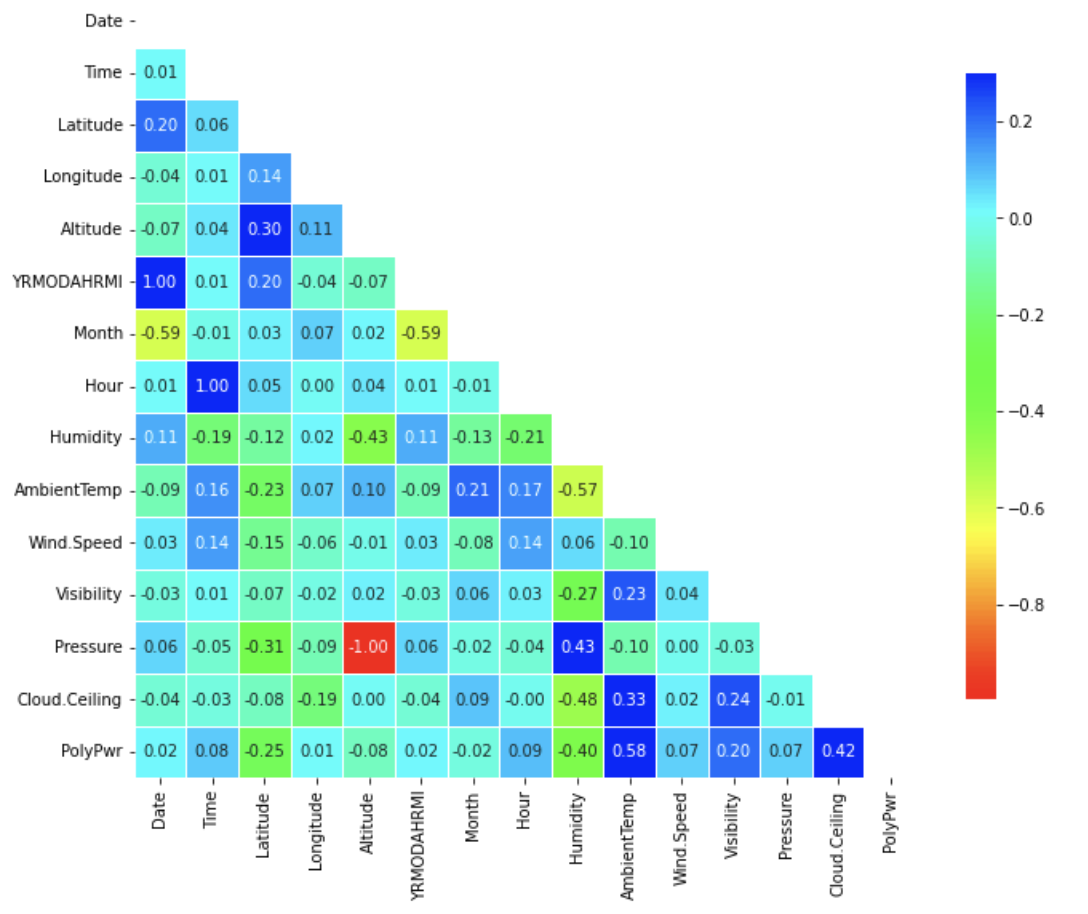
\includegraphics[width=10cm, height=5.8cm] {corr.png}
    \caption{Correlation between available features}
    \label{fig:my_label}
\end{figure}
\hfill \break 
\\
The analysis of the data in the plot above shows that there is a high negative correlation between humidity and ambient temperature. This is because when the temperature is high, the air becomes dry, leading to a decrease in humidity. Humidity is defined as the ratio of the actual water vapor pressure to the maximum or saturation water vapor pressure in a stable temperature. Therefore, the high correlation between humidity and temperature is due to the fact that when the temperature is stable, humidity depends only on pressure. Additionally, the amount of cloud cover can impact the temperature. When there are more clouds, less sunlight is received by the Earth, which leads to a decrease in temperature. However, the height of the cloud ceiling can also impact the temperature. When the clouds are situated at a higher altitude, they can reflect the sun's rays back through the Earth, causing an increase in temperature. This can explain the high correlation between humidity and temperature in the dataset. Overall, these findings suggest that humidity and ambient temperature are closely related and can be used to better understand the atmospheric conditions of a given environment.\\
\\
Before explaining the other correlations between the data, let stop on an important point. The Location should have a high impact on the data but due to its format it's not checked in the correlation analyses. Subsequently, correlation plots will be presented for each location. Figure 4.5 shows the different values of the location feature and the count of each value.
\begin{figure}[h!]
  \centering
    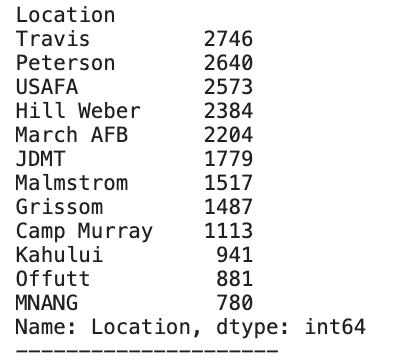
\includegraphics[width=8cm, height=6.5cm] {count.png}
    \caption{Location values}
    \label{fig:my_label}
\end{figure} \newpage
\hfill \break 
\\
There are a total of 12 distinct values for the location feature. Travis, Peterson, USAFA, Hill Weber, March AFB, JDMT, Malmsrom, Grissom, Camp Murray, Kahului, Offutt, and MNANG. Each location is far from the other one with at least 100 km which means that its has a huge impact on the other features. And the next figures represents the correlation plot of each location.\hfill \break 
\\
\\
\begin{figure}[h!]
    \centering
    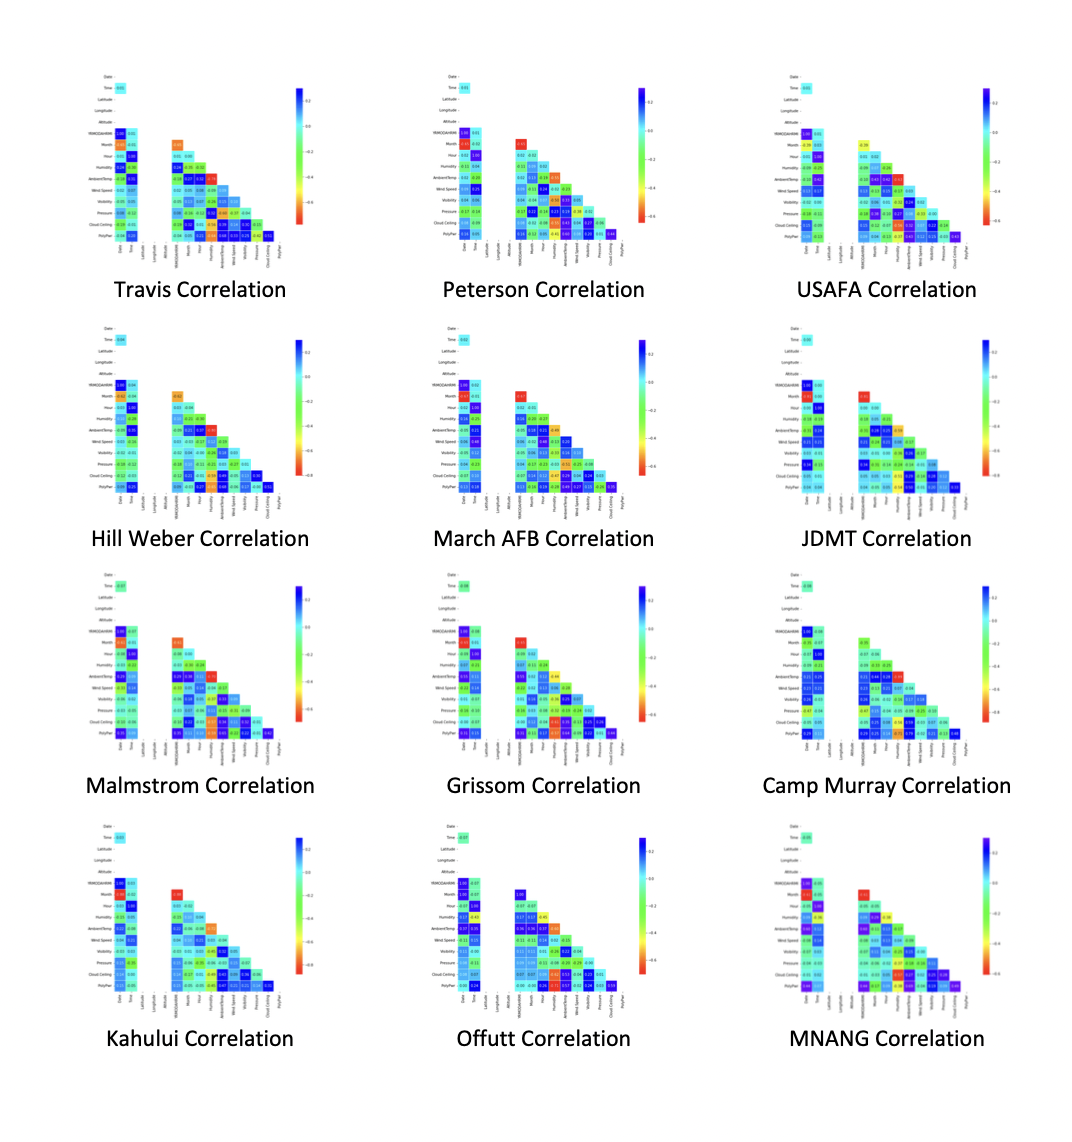
\includegraphics[width=12cm, height=12cm]{1234.png}
    \caption{Features Correlation}
\end{figure}\newpage \hfill \break 
\\
Based on the above figures, it can be concluded that the location feature is crucial, given that the correlation between the features, especially between the features and the Polypower, changes significantly. As a result, the location feature must be encoded during the pre-processing stage. Additionally, it can be observed that the three features, Longitude, Latitude, and Altitude, do not exist, meaning that for this location, these values are identical. In Figure 4.4, a perfect correlation can be seen between Pressure and Altitude. Hence, this column will be removed since its value remains constant for all rows in the same location.\hfill \break 
\\ 
The correlation between the target feature, Polypower, and the other features will now be examined. This correlation will be illustrated in Figure 4.7.
\begin{figure}[h!]
  \centering
    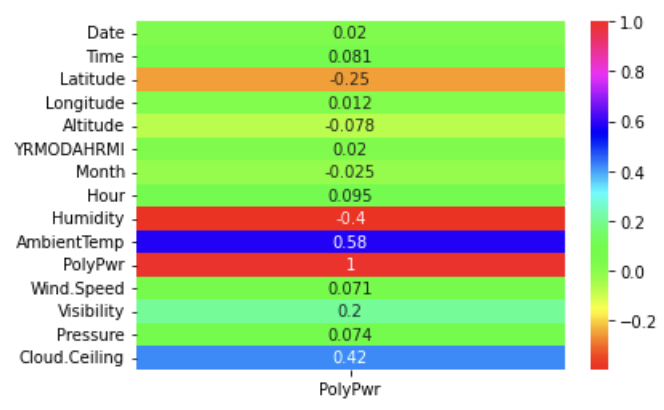
\includegraphics[width=7cm, height=5cm] {polycorr.png}
    \caption{Power correlation}
    \label{fig:my_label}
\end{figure}\hfill \break
\\
The figure presented above provides evidence of a high correlation between power and three variables: temperature, humidity, and cloud ceiling. The plot illustrates a clear positive relationship between power and these three variables. As temperature and humidity increase, so does power consumption. Additionally, a high cloud ceiling is associated with an increase in power consumption. This relationship can be explained by the fact that as temperature and humidity increase, the demand for cooling and air conditioning also increases, which leads to a rise in power consumption. Similarly, a high cloud ceiling can indicate an increase in solar radiation, which can cause an increase in temperature and a subsequent increase in power consumption. These findings have important implications for energy management and suggest that understanding the relationship between weather conditions and power consumption is essential for optimizing energy efficiency. By identifying the key weather variables that impact power consumption, it may be possible to develop more accurate models for predicting energy demand and improving energy management strategies.
\section{Data Pre-processing}
Initially, the YRMODAHRMI, Longitude, and Altitude columns will be removed. Subsequently, the data will be checked for any missing values. Figure 4.33 depicts that the data does not contain any missing values.
\begin{figure}[h!]
  \centering
    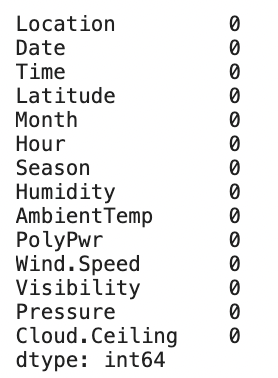
\includegraphics[width=6cm, height=5.5cm] {mv.png}
    \caption{Missing values}
    \label{fig:my_label}
\end{figure}\hfill \break
\\
The figure above depicts a dataset with 0 missing values in all of its features. This is a highly desirable outcome, as missing data can often lead to biased or inaccurate analyses. A dataset with no missing values allows for a more complete and accurate understanding of the relationships between variables and can improve the effectiveness of statistical models and machine learning algorithms. 
\subsection{Outliers}
Outliers are the values that are far from the rest of the data. They can be caused by measurement errors or they can be real values. Box plots are useful to detect outliers within a data set. The next figures present the box-plots of the features of our data.
\begin{figure}[h!]
    \centering
    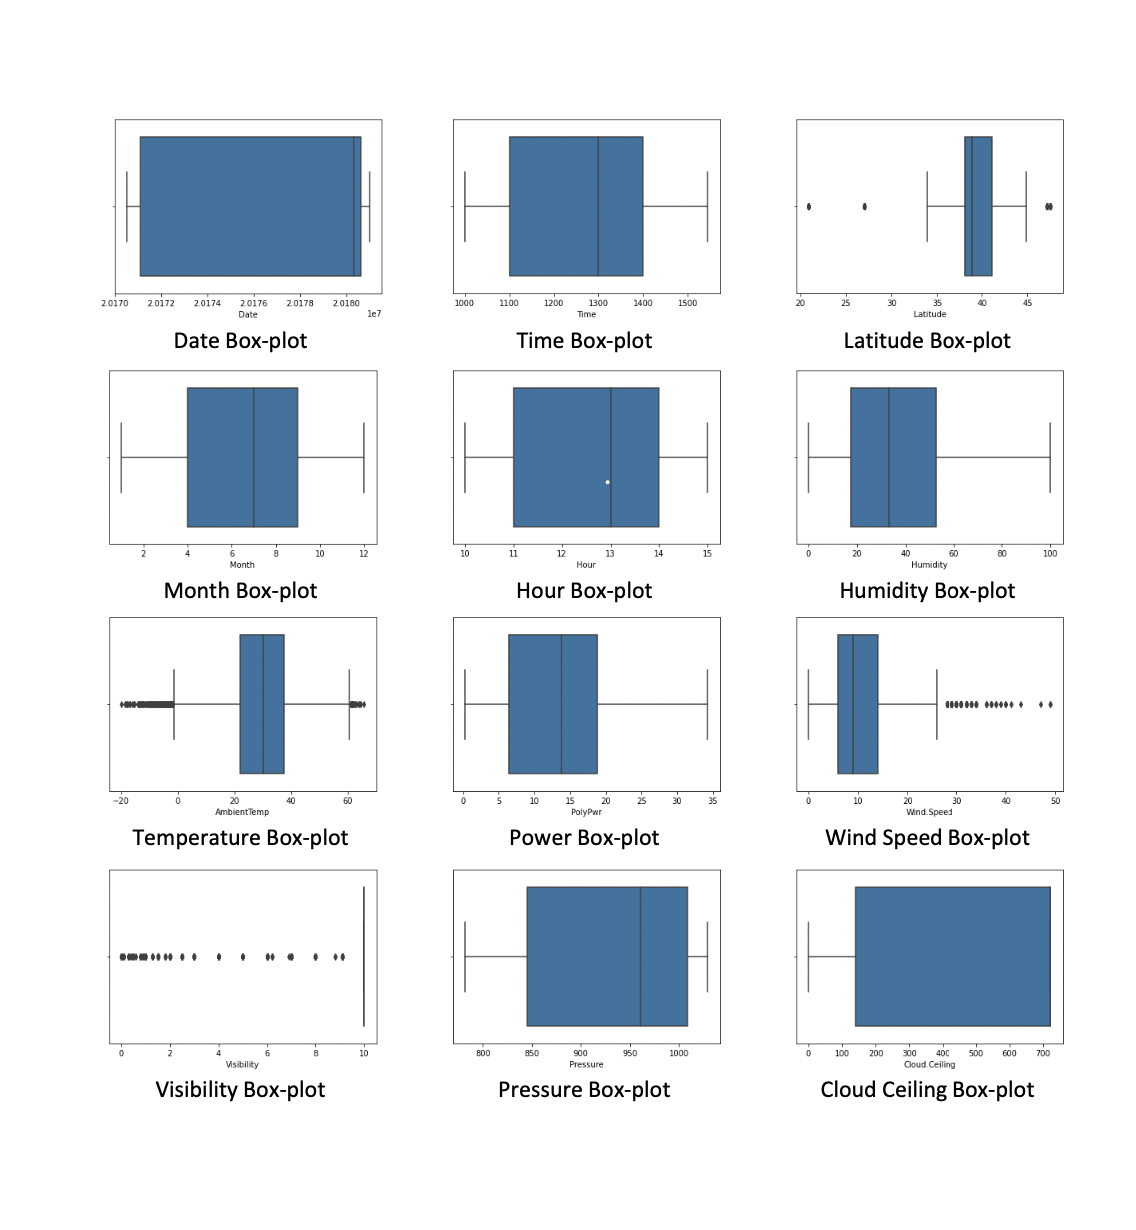
\includegraphics[width=12cm, height=12cm]{1111.png}
    \caption{Features Box-Plot}
\end{figure}\newpage \hfill \break 
\\
Figures above outlines the approach that will be taken to address outliers in the temperature and wind speed features of the dataset. Firstly, temperature outliers above 60 and under -10 will be eliminated as these values are outside the normal range of ambient temperature. The values where the temperature value is between the lower bound and -10 are considered true outliers and will also be removed. Similarly, wind speed outliers above 30 will be eliminated as they are outside the normal range of wind speed. However, instead of eliminating outliers, their values will be replaced with the mean or median, depending on the nature of the data in each location. Box plots for both wind speed and ambient temperature will be created for each location to determine whether the outliers should be replaced with the mean or median. The approach of replacing outliers with the mean or median is being taken as the box plots of both features showed a low distance between the first and third quartiles, indicating that the data values are very close. Box plots for each location will be created for both the wind speed and ambient temperature features to determine the appropriate replacement method for outliers.
\begin{figure}[h!]
    \centering
    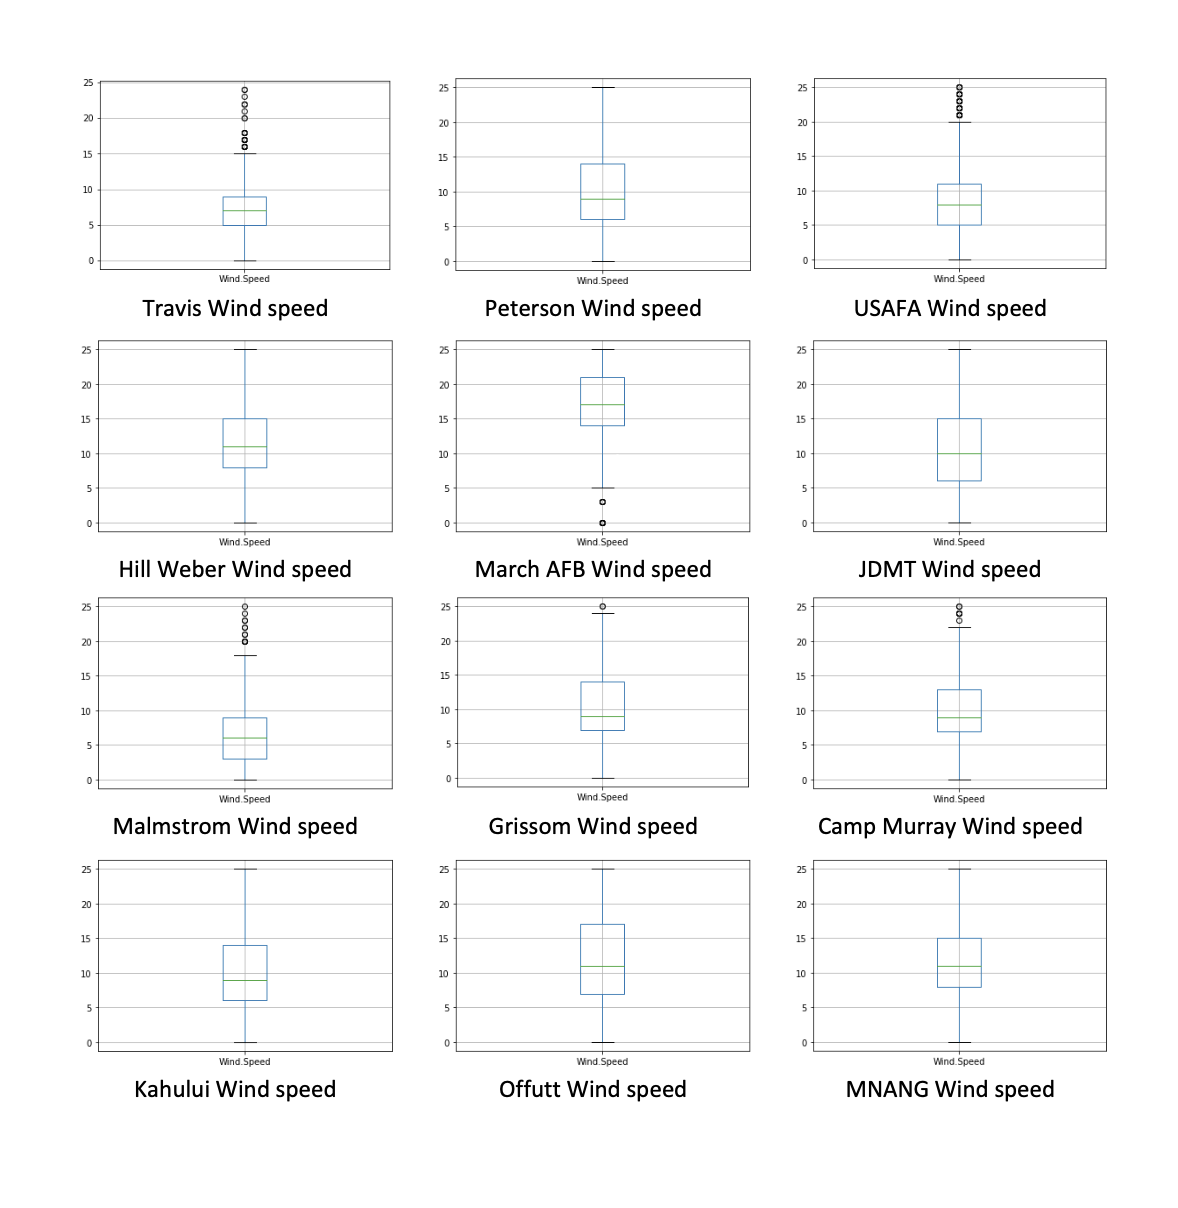
\includegraphics[width=12cm, height=12cm]{2222.png}
    \caption{Wind Speed Box-Plot For Each Location}
\end{figure}\newpage \hfill \break 
\\
The analysis of the figures presented above revealed the presence of outliers in the wind speed feature across six different locations, namely Travis, USAFA, March AFB, Malmstrom, Grissom, and Camp Murray. In order to address the issue of outliers and ensure the accuracy of the data, different methods of replacement were employed depending on the nature of the data in each location. Specifically, the data distribution in Travis, USAFA, and Malmstrom was found to be normal, with the mean being equal to the median. Therefore, it is appropriate to replace the outliers in these locations with the mean. On the other hand, the data in March AFB was positively skewed, with outliers located in the lower bound. In this case, replacement with the median is appropriate. In Camp Murray and Grissom, the data was also positively skewed, but the outliers were located in the upper bound. Therefore, replacing the outliers with the mean is appropriate in these locations. By replacing the outliers with either the mean or median, as appropriate, in each location, the data can be more accurately represented and analyzed.
\begin{figure}[h!]
    \centering
    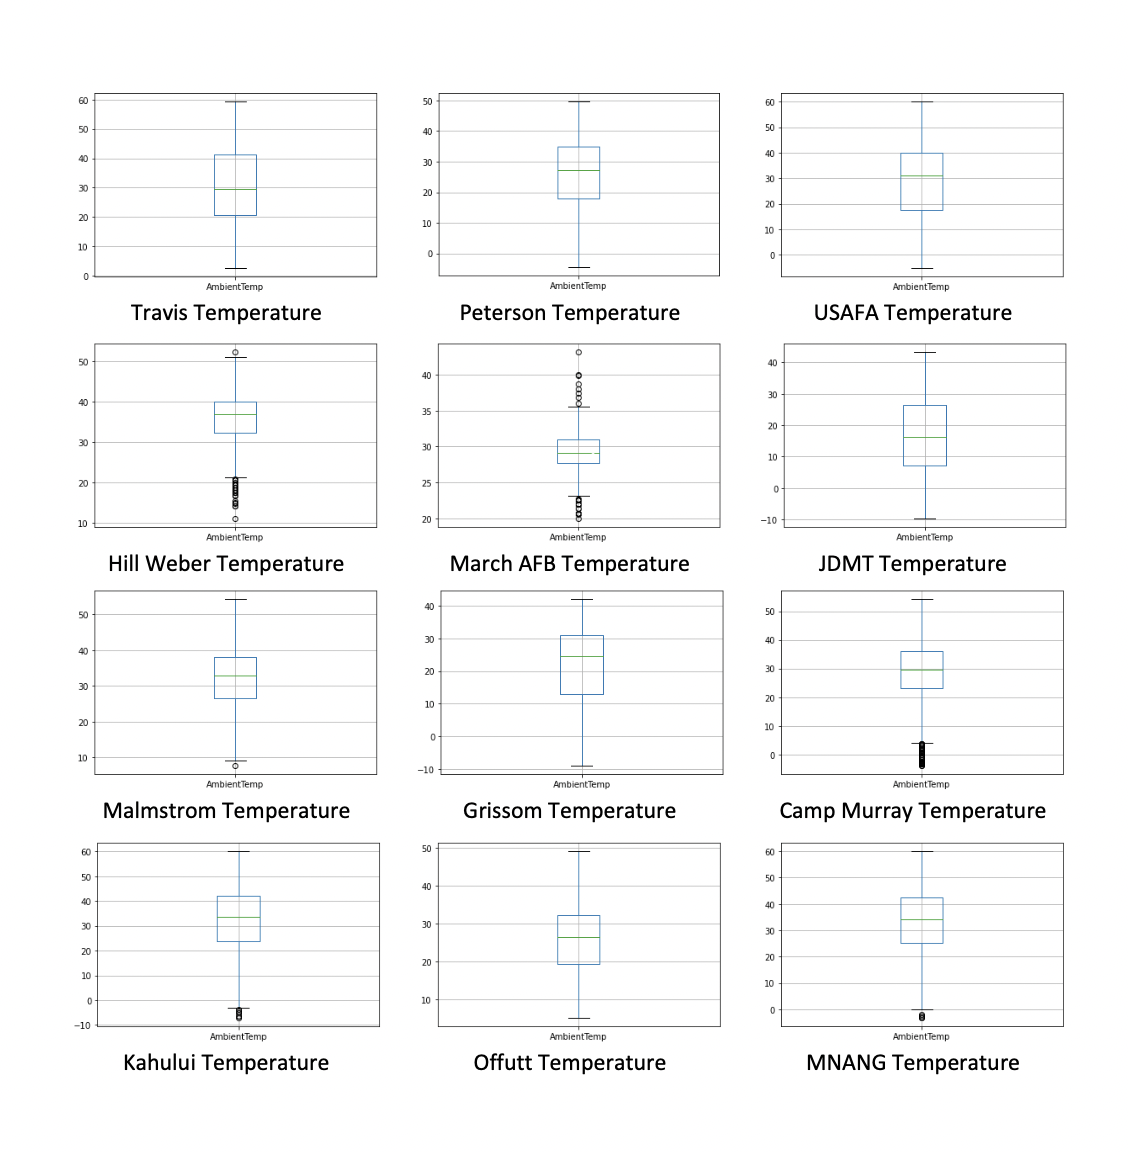
\includegraphics[width=12cm, height=12cm]{3333.png}
    \caption{Temperature Box-Plot For Each Location}
\end{figure}\newpage \hfill \break 
\\
Outliers were identified in the ambient temperature feature in six locations: Hill Weber, March AFB, Malmstrom, Camp Murray, Kahului, and MNANG. The data distribution in MNANG, Camp Murray, Kahului, and March AFB was normal, with the mean being equal to the median. Therefore, in these locations, replacing outliers with the mean is appropriate. In Hill Weber and Malmstrom, the data was negatively skewed, with outliers located in the lower bound. In these locations, replacement with the mean is appropriate. Hence, the outliers in the ambient temperature feature will be replaced with the mean in Hill Weber and Malmstrom, while in the remaining locations, the outliers will be replaced with either the mean or median, as appropriate.
\subsection{Data Encoding}
When dealing with categorical data, the data is typically stored as strings. However, this can lead to issues when attempting to apply mathematical algorithms to the data. To avoid these problems, it is necessary to encode the data using one of the following methodologies:
\begin{itemize}
    \item Nominal encoding : This is the simplest approach and it is used when the order in the category doesn’t matter. Different techniques are used in nominal encoding such as:    \begin{itemize}
        \item One hot encoding : is a popular method for encoding categorical data. This technique uses a binary column to represent each category. While it is an efficient method, one-hot encoding has a major disadvantage in that it typically creates very sparse data. As a result, one-hot encoding is best used for categorical variables with a small number of categories.
        \item Mean Encoding: is a technique for encoding categorical data, which involves creating a column for each category and storing the mean value of the feature for that category. However, this approach is not very memory-efficient, and it may not be as accurate as other encoding techniques.
        \item Label Encoding:  is a technique for encoding categorical data, which involves creating a column for each category and storing the category label. However, this approach is not very memory-efficient and may not be as accurate as other encoding techniques.
    \end{itemize}
    \item Ordinal encoding: is a type of categorical data encoding that is a special case of nominal encoding. In ordinal encoding, the order of the categories is significant. The same techniques used in nominal encoding can be applied, but it is essential to consider the order of the categories.
\end{itemize}
The data set contains two categorical features: Location and Season. One-hot encoding will be used for Location since it has only a few categories. For Season, the power revenue follows the order Summer $>$ Spring $>$ Fall $>$ Winter, so an ordinal encoding will be used, with Summer being assigned the value of 4, Spring the value of 3, Fall the value of 2, and Winter the value of 1.

\subsubsection{Cyclical Encoding}
The data contains a cyclic feature such as the hour of the day which repeats after every 24 hours. However, this presents an issue in the model, where the difference between the values of the feature is not accurately represented. For instance, the difference between 23h and 00h would be considered as 23h by the model instead of 1h. To resolve this issue, the feature must be encoded using cyclical encoding. This involves normalizing the feature values to a range of 0 to 2{$\pi$} and then computing the cosine of the resulting values. \hfill \break 
\\
To encode the Time feature, the HHMM value must be transformed to a float number using the following equation:
\begin{equation}
    HHMM = HH\times(\frac{100}{24})\times100 + MM\times(\frac{100}{60})
\end{equation}
The values of the date features were normalized between 0 and 2$\pi$ in order to calculate the cosine. The graph of the resulting feature is presented in Figure 4.12.
\begin{figure}[h!]
  \centering
    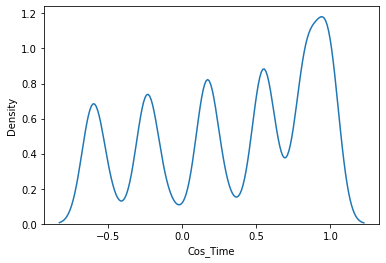
\includegraphics[width=12cm, height=6cm] {aaa.png}
    \caption{Cosine of normalized Time feature}
    \label{fig:my_label}
\end{figure}
\hfill \break 
Figure 4.12 shows the graph of the cosine function of the normalized Time feature. It is noted that for certain values of Time, such as 0.5, there are multiple corresponding values of the cosine function. To address this issue, a new feature is created that presents the sine function, which is also graphed in Figure 4.13.\hfill \break 
\begin{figure}[h!]
  \centering
    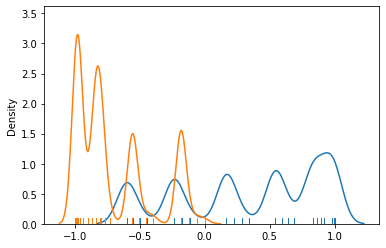
\includegraphics[width=12cm, height=6cm] {bbb.png}
    \caption{Sine of normalized Time feature}
    \label{fig:my_label}
\end{figure} \newpage
\hfill \break 
Figure 4.13 shows the graph of the sine function. The addition of the sine feature allows for unique values to be assigned to each time point, which is important for accurate data analysis. Overall, the addition of the sine feature is a useful approach for avoiding duplicate values in the dataset and ensuring accurate analysis of the data.\\
\\
The same process will be applied to the Date feature. The cosine and sine features are displayed in the two following figures:\hfill \break 
\\
\begin{figure}[h!]
  \centering
  \begin{minipage}[b]{0.45\textwidth}
    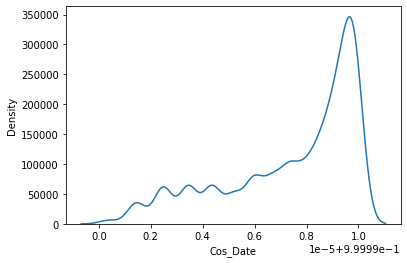
\includegraphics[width=\textwidth]{cs.png}
    \caption{Cosine of normalized Date feature}
  \end{minipage}
  \hfill
  \begin{minipage}[b]{0.45\textwidth}
    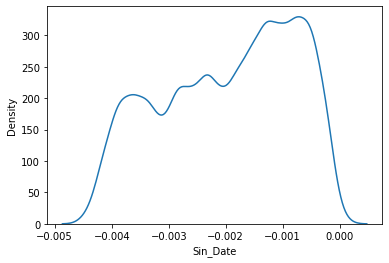
\includegraphics[width=\textwidth]{sn.png}
    \caption{Sine of normalized Date feature}
  \end{minipage}
\end{figure}\break
Figure 4.14 and Figure 4.15 shows the graph both the cosine and sine functions of the normalized Time feature together.\\
\\
The Hour feature contains values between 10 and 15, and based on the knowledge that the average of the maximum temperature is in the afternoon , essentially the model will take it as an order data where 15 is the highest value. But as the conductors of the photovoltaic panel take just the needed quantity of energy and transform the rest into heat, the panel´s internal temperature will increase and at a given level will affect the power out. To increase the model accuracy, another feature will be created from the ambient temperature, this feature will be the time range of the hour feature so the model can know how many hours it had been working. Let's plot the correlation between all the features that include the encoded features. 
\begin{figure}[h!]
  \centering
    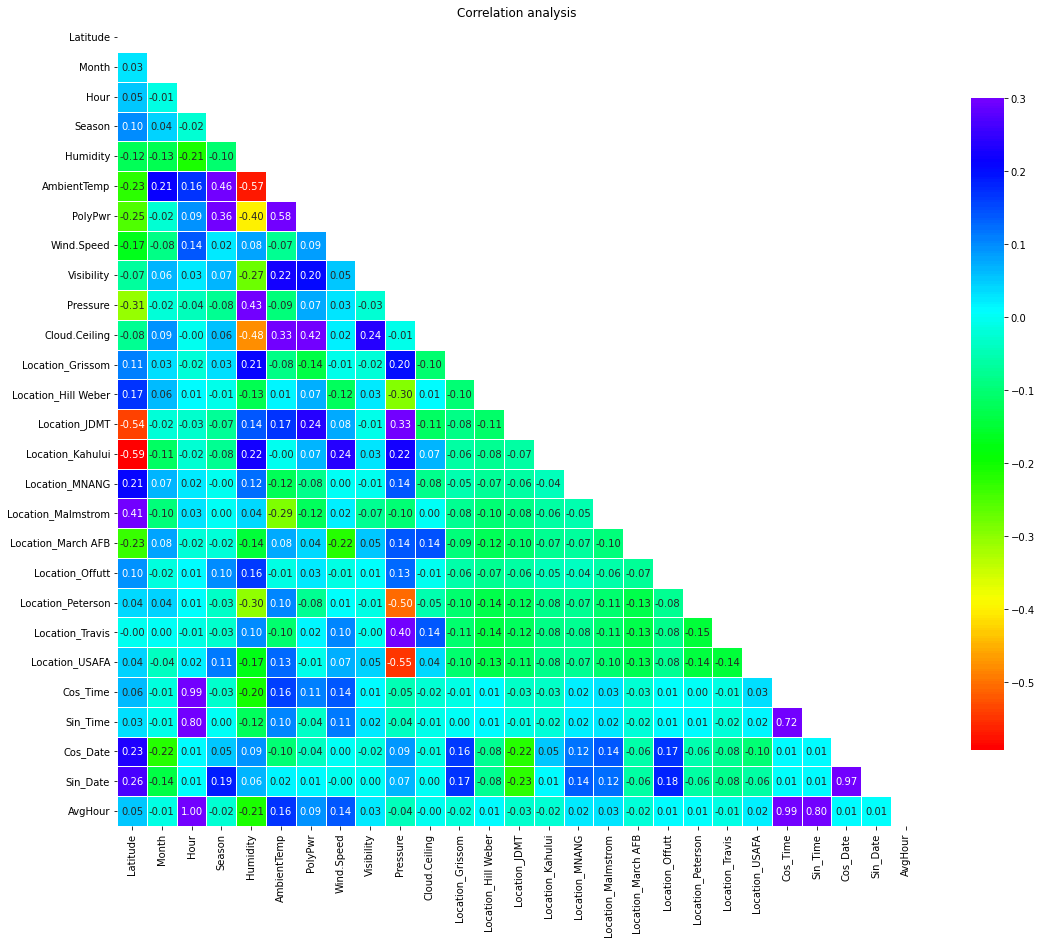
\includegraphics[width=14cm, height=9cm] {cf.png}
    \caption{Correlation between all the features including the encoded features}
    \label{fig:my_label}
\end{figure}
\hfill \break 
\\
The figure above presents the correlation between all the features. According to Figure 4.16, the correlation between the Hour feature and other features is shown to be equivalent to that of the AvgHour feature and other features. Therefore, it is recommended that the Hour feature be dropped in favor of the AvgHour feature, as it provides more information that may be useful for future work. The correlation between the weather features and the encoded location feature is observed to vary between different locations due to the change in location. Additionally, there is a strong correlation observed between the season and both the weather temperature and Polypower. These findings suggest that location and season are important factors to consider in analyzing the data and drawing meaningful conclusions.
\subsubsection{Pipeline}
Because many changes were made to the data, a potential issue that could arise when splitting it into training and testing sets is a difference in distribution between the two sets. In order to ensure that the training and testing data are normalized in the same way and thus able to be used for comparing models, a pipeline will be employed. This pipeline will normalize the data and encode any categorical features, and is essentially a single scikit-learn estimator that chains together multiple processing steps.\\
The pipeline will be composed of the following steps:
\begin{itemize}
    \item One hot encoding for the Location feature.
    \item Ordinal encoding for the Season feature.
    \item Cyclical encoding for the Time and Date features.
    \item Data scaling.
\end{itemize}

\section{Model Creation and Implementation}
\subsection{Model Selection}
Prior to model selection, it is important to note that in the feature encoding step, cyclical features were encoded using the normalized cosine and sine values, resulting in two features for each cyclical feature. Since decision tree-based models process the data on a feature-by-feature basis, employing decision tree models may not be optimal for this dataset.\cite{ce}
\subsubsection{Linear Models}


Linear models are a good choice for our problem because they are fast to train and they are easy to interpret. They are also good for high-dimensional data. The linear models that will be used are:
\begin{itemize}
    \item Linear Regression: is a linear approach for modeling the relationship between a scalar response and one or more explanatory variables. The case of one explanatory variable is called simple linear regression. The process is called multiple linear regression for more than one explanatory variable. \cite{scikit-learn} The model is defined by the following equation:
    \begin{equation}
        y = w_0 + w_1x_1 + w_2x_2 + ... + w_nx_n
    \end{equation}
    \item Ridge Regression: is a linear model that incorporates L2 regularization, which involves adding a penalty term to the loss function. This penalty term is calculated as the sum of the squared values of the model coefficients. Ridge Regression is an effective model for reducing model complexity when faced with a large number of features\cite{scikit-learn}.  The model is defined by the following equation:
    \begin{equation}
        y = w_0 + w_1x_1 + w_2x_2 + ... + w_nx_n + \alpha \sum_{i=1}^{n} w_i^2
    \end{equation}
    \item Lasso Regression: is a linear model that utilizes L1 regularization, which adds a penalty term to the loss function that is calculated as the sum of the absolute values of the model coefficients. Lasso Regression is a suitable model for reducing model complexity in datasets with a large number of features\cite{scikit-learn}. The model is defined by the following equation:
    \begin{equation}
        y = w_0 + w_1x_1 + w_2x_2 + ... + w_nx_n + \alpha \sum_{i=1}^{n} |w_i|
    \end{equation}
    \item Elastic Net: is a linear model that incorporates both L1 and L2 regularization techniques. It is an appropriate model for reducing model complexity in datasets with a large number of features\cite{scikit-learn}. The model is defined by the following equation:
    \begin{equation}
        y = w_0 + w_1x_1 + w_2x_2 + ... + w_nx_n + \alpha \sum_{i=1}^{n} |w_i| + \alpha \sum_{i=1}^{n} w_i^2
    \end{equation}
\end{itemize}
\subsubsection{Non-Linear Models}
Non-linear models are more complex than linear models, but they can capture more complex patterns in the data. The non-linear models that will be use are:
\begin{itemize}
    \item Support Vector Machine for Regression: is a non-linear model that uses the kernel trick to transform the data into a higher dimension. Then it uses the transformed data to find the best hyperplane that separates the data. These hyperplanes are called support vectors\cite{scikit-learn} . 
    \item K-Nearest Neighbors for Regression: is a non-linear model that uses the distance between the data points to find the nearest neighbors. Then it uses the neighbors to predict the value of the data point\cite{scikit-learn}. 
\end{itemize}
\subsubsection{Neural Network}
Neural networks are a suitable option for handling high dimensional data, data with a significant amount of noise, and datasets with a large number of features. However, in this case, the use of neural networks may not be optimal due to the small dataset. Despite this, the multi-layer perceptron regressor will be employed to gain insight into the potential performance of neural network models for future work. The multi-layer perceptron regressor is defined by the following equation:
\begin{equation}
    y = f(w_0 + w_1x_1 + w_2x_2 + ... + w_nx_n)
\end{equation}
\subsubsection{Stacking Regressor}
Stacking is a technique that uses multiple models to make a prediction. The models are trained on the same data, and then the predictions are combined to make the final prediction. The model is defined by the following equation:
\begin{equation}
    y = \sum_{i=1}^{n} w_i f_i(x)
\end{equation}
\subsection{Model Evaluation}
\subsubsection{Cross Validation}
Cross-validation is a technique that is used to evaluate the performance of a model. It is used to avoid overfitting and to make sure that the model is not biased. The cross-validation technique that will be used is the K-fold cross-validation. In this technique, the data is split into K folds. Then the model is trained K times, each time using a different fold as the testing set and the rest of the folds as the training set. The final score is the average of the K scores\cite{scikit-learn}.
\subsubsection{Metrics}
The metrics that will be used to evaluate the models are:
\begin{itemize}
    \item Mean Absolute Error (MAE) : is the average of the absolute differences between the predictions and the actual values. MAE is a suitable metric to use when the data contains outliers\cite{scikit-learn}. 
    \item Mean Squared Error (MSE) : is the average of the squared differences between the predictions and the actual values. MSE is a suitable metric to use when there are no outliers in the data\cite{scikit-learn}. 
    \item R2 Score: also known as the coefficient of determination, is a metric that provides information on the proportion of variance in the data that is explained by the model. R2 Score is an appropriate metric to use when the objective is to assess the model's ability to explain the variability in the data\cite{scikit-learn}. 
\end{itemize}
\section{Results}
\subsection{Linear Models}
\subsubsection{Linear Regression}
\begin{table}[h]
\centering
\begin{tabular}{|c|c|c|c|}
\hline
\textbf{Metric} & \textbf{Value} \\ \hline
Mean Absolute Error & 3.5945 \\ \hline
Mean Squared Error & 22.1607 \\ \hline
R2 Score & 0.5629 \\ \hline
\end{tabular}
\caption{Linear Regression Results}
\end{table}
\break \hfill 
\\
Table 4.1 presents the performance of linear regression model. The model has a MAS of 3.5945, an MSS of 22.1607, and an R-squared value of 0.5629.
\subsubsection{Ridge Regression}
\begin{table}[h]
\centering
\begin{tabular}{|c|c|c|c|}
\hline
\textbf{Metric} & \textbf{Value} \\ \hline
Mean Absolute Error & 3.5943 \\ \hline
Mean Squared Error & 22.1584 \\ \hline
R2 Score & 0.5630 \\ \hline
\end{tabular}
\caption{Ridge Regression Results}
\end{table}
\hfill \break
\\
Table 4.2 presents the performance of a ridge regression model. The model has a MAS of 3.5943, an MSS of 22.1584, and an R-squared value of 0.5630.
\subsubsection{Lasso Regression}
\begin{table}[h]
\centering
\begin{tabular}{|c|c|c|c|}
\hline
\textbf{Metric} & \textbf{Value} \\ \hline
Mean Absolute Error & 4.5193 \\ \hline
Mean Squared Error & 30.6571 \\ \hline
R2 Score & 0.3954 \\ \hline
\end{tabular}
\caption{Lasso Regression Results}
\end{table}
\hfill \break
\\
Table 4.3 presents the performance of a lasso regression model. The model has a MAS of 4.5193, an MSS of 30.6571, and an R-squared value of 0.3954.
\subsubsection{Elastic Net}
\begin{table}[h]
\centering
\begin{tabular}{|c|c|c|c|}
\hline
\textbf{Metric} & \textbf{Value} \\ \hline
Mean Absolute Error & 4.4210 \\ \hline
Mean Squared Error & 29.0551 \\ \hline
R2 Score & 0.4270 \\ \hline
\end{tabular}
\caption{Elastic Net Results}
\end{table}
\hfill \break
\\
Table 4.4 presents the performance of an elastic net model. The model has a MAS of 4.4210, an MSS of 29.0551, and an R-squared value of 0.4270.
\subsection{Non-Linear Models}
\subsubsection{Support Vector Machine for Regression}
\begin{table}[h]
\centering
\begin{tabular}{|c|c|c|c|}
\hline
\textbf{Metric} & \textbf{Value} \\ \hline
Mean Absolute Error & 2.7350 \\ \hline
Mean Squared Error & 18.3983 \\ \hline
R2 Score & 0.6372 \\ \hline
\end{tabular}
\caption{Support Vector Machine for Regression Results}
\end{table}
\hfill \break
\\
Table 4.5 presents the performance of a support vector machine (SVM) regression model. The model has a MAS of 2.7150, an MSS of 18.3983, and an R-squared value of 0.6372.
\subsubsection{K-Nearest Neighbors for Regression}
\begin{table}[h]
\centering
\begin{tabular}{|c|c|c|c|}
\hline
\textbf{Metric} & \textbf{Value} \\ \hline
Mean Absolute Error & 2.9926 \\ \hline
Mean Squared Error & 20.1517 \\ \hline
R2 Score & 0.6023 \\ \hline
\end{tabular}
\caption{K-Nearest Neighbors for Regression Results}
\end{table}
\hfill \break
\\
Table 4.6 presents the performance of a K-nearest neighbor (KNN) regression model. The model has a MAS of 2.9926, an MSS of 20.1517, and an R-squared value of 0.6023.
\subsection{Neural Network}
\begin{table}[h]
\centering
\begin{tabular}{|c|c|c|c|}
\hline
\textbf{Metric} & \textbf{Value} \\ \hline
Mean Absolute Error & 2.7909 \\ \hline
Mean Squared Error & 16.8960 \\ \hline
R2 Score &  0.6679 \\ \hline
\end{tabular}
\caption{Neural Network Results}
\end{table}
\hfill \break
\\
Table 4.7 presents the performance of a neural network regression model. The model has a MAS of 2.7909, an MSS of 16.8969, and an R-squared value of 0.6679.
\subsection{Stacking Regressor}
\begin{table}[h]
\centering
\begin{tabular}{|c|c|c|c|}
\hline
\textbf{Metric} & \textbf{Value} \\ \hline
Mean Absolute Error & 2.9039 \\ \hline
Mean Squared Error & 18.9112 \\ \hline
R2 Score &  0.6301 \\ \hline
\end{tabular}
\caption{Stacking Regressor Results}
\end{table}
\hfill \break
\\
Table 4.8 presents the performance of a stacking regressor model. The model has a MAS of 2.9039, an MSS of 18.9112, and an R-squared value of 0.6301. Stacking is an ensemble learning technique that combines multiple regression models to improve their overall performance.\\
\\
The support vector machine (SVM) regression model has the lowest Mean Absolute Square (MAS) and Mean Squared Square (MSS) values, indicating better accuracy in predicting the target variable. It also has the highest R-squared value, indicating that it explains the highest proportion of the variation in the dependent variable. The neural network model and the K-nearest neighbor (KNN) regression model also performed well, with relatively low MAS and MSS values and high R-squared values.\\
\\
The linear regression, ridge regression, and elastic net models performed relatively poorly compared to the other models. The lasso regression model performed the worst, with the highest MAS and MSS values and the lowest R-squared value.\\
\\
Finally, the stacking regressor model performed well, with low MAS and MSS values and a high R-squared value.\\
\\
In conclusion, the support vector machine (SVM) regression model, the neural network model, and the K-nearest neighbor (KNN) regression model are the best performing models for the given dataset, while the lasso regression model is the worst performing model. However, the stacking regressor model also performed well and is worth considering as an option. Therefore, a hyperparameter tuning should be performed to optimize the performance of these models further. 
\subsection{Hyperparameter Tuning}
Hyperparameters are parameters that pertain to the model itself, rather than the data. They are utilized to control the model, and are not learned by the model, but rather set by the user. To determine the optimal hyperparameters for a model, various techniques can be employed, including Grid Search. This technique involves defining a grid of hyperparameters, and then training the model for each combination of hyperparameters. The best combination of hyperparameters is determined by the one that yields the highest score\cite{scikit-learn}. 
\subsubsection{Support Vector Machine for Regression}
\begin{itemize}
    \item kernel: is the kernel type to be used in the algorithm. It can be ‘linear’, ‘poly’, ‘rbf’, ‘sigmoid’, ‘precomputed’, or a callable. The linear kernel is the default one\cite{scikit-learn}. 
    \item C: is the penalty parameter C of the error term. It controls the trade-off between smooth decision boundaries and classifying the training points correctly. If C is too low, the penalty for miss-classifying the training points is too low and the model will not be able to learn the data. If C is too high, the penalty for miss-classifying the training points is too high and the model will overfit the data\cite{scikit-learn}. 
    \item gamma: is the kernel coefficient for ‘rbf’, ‘poly’, and ‘sigmoid’. If gamma is ‘auto’ then 
    \begin{equation}
    \centering
        \frac{1}{n_{features}}
    \end{equation} 
    will be used instead. If gamma is ‘scale’ then 
    \begin{equation}
        \frac{1}{n_{features} \times X.var()}
    \end{equation} will be used instead\cite{scikit-learn}. 
\end{itemize}
Results of the Grid Search:
\begin{table}[h]
\centering
\begin{tabular}{|c|c|c|c|}
\hline
\textbf{Hyperparameter} & \textbf{Value} \\ \hline
kernel & rbf \\ \hline
C & 100 \\ \hline
gamma & scale \\ \hline
\end{tabular}
\caption{Support Vector Machine for Regression Hyperparameter Tuning Results}
\end{table} \\
\\
Table 4.9 shows the hyperparameters and their corresponding values for a support vector machine (SVM) regression model. The kernel used for this model is the radial basis function (rbf), which is a popular kernel for SVMs. The C value is set to 100, which controls the trade-off between achieving a low training error and a low testing error. The gamma value is set to 'scale', which means that it is calculated as the inverse of the number of features in the input data. Gamma determines the influence of a single training example on the decision boundary. 
\subsubsection{K-Nearest Neighbors for Regression}
\begin{itemize}
    \item n\_neighbors: is the number of neighbors to use by default for kneighbors queries\cite{scikit-learn}. 
    \item weights: is the weight function used in prediction. Possible values: ‘uniform’: uniform weights. All points in each neighborhood are weighted equally. ‘distance’: weight points by the inverse of their distance. in this case, closer neighbors of a query point will have a greater influence than neighbors who are further away\cite{scikit-learn}. 
    \item algorithm: is the algorithm to be used by the NearestNeighbors module to compute pointwise distances and find nearest neighbors.
    \item leaf\_size: is the leaf size passed to BallTree or KDTree. This can affect the speed of the construction and query, as well as the memory required to store the tree. The optimal value depends on the nature of the problem\cite{scikit-learn}. 
\end{itemize}
Results of the Grid Search:
\begin{table}[h]
\centering
\begin{tabular}{|c|c|c|c|}
\hline
\textbf{Hyperparameter} & \textbf{Value} \\ \hline
n\_neighbors & 10 \\ \hline
weights & distance \\ \hline
algorithm & auto \\ \hline
leaf\_size & 10 \\ \hline
\end{tabular}
\caption{K-Nearest Neighbors for Regression Hyperparameter Tuning Results}
\end{table}\\
\\
Table 4.10 shows the hyperparameters and their corresponding values for a K-nearest neighbors (KNN) regression model, which has been tuned for optimal performance. The hyperparameter 'n\_neighbors' is set to 10, which specifies the number of neighbors to consider when making a prediction. The 'weights' hyperparameter is set to 'distance', which weights the contributions of the neighbors according to their distance. The 'algorithm' hyperparameter is set to 'auto', which means that the algorithm automatically chooses the best algorithm based on the input data. Finally, the 'leaf\_size' hyperparameter is set to 10, which is the number of points at which the algorithm switches to brute-force search. 
\subsubsection{Linear Regression}
\begin{itemize}
    \item fit\_intercept : whether to calculate the intercept for this model. If set to False, no intercept will be used in calculations (i.e. data is expected to be already centered)\cite{scikit-learn}. 
    \item n\_jobs : is the number of jobs to use for the computation. This will only provide speedup for n\_targets > 1 and sufficient large problems\cite{scikit-learn}. 
    \item copy\_X : If True, X will be copied; else, it may be overwritten\cite{scikit-learn}. 
    \item positive : When set to True, forces the coefficients to be positive\cite{scikit-learn}. 
\end{itemize}
Results of the Grid Search:
\begin{table}[h]
\centering
\begin{tabular}{|c|c|c|c|}
\hline
\textbf{Hyperparameter} & \textbf{Value} \\ \hline
fit\_intercept & True \\ \hline
n\_jobs & None \\ \hline
copy\_X & True \\ \hline
positive & False \\ \hline
\end{tabular}
\caption{Linear Regression Hyperparameter Tuning Results}
\end{table}\\
\\
Table 4.11 shows the hyperparameters and their corresponding values for a linear regression model, which has been tuned for optimal performance. The hyperparameter 'fit\_intercept' is set to True, which specifies whether or not to calculate the intercept for the model. The 'n\_jobs' hyperparameter is set to None, which means that the number of parallel jobs to use for the computation is set to the number of CPU cores. The 'copy\_X' hyperparameter is set to True, which means that a copy of the input X data is made. The 'positive' hyperparameter is set to False, which means that the coefficients are not constrained to be positive. 
\subsubsection{Ridge Regression}
For this model, the same hyperparameters will be used as the Linear Regression model, with the exception of n\_jobs, in addition to the following hyperparameter:
\begin{itemize}
    \item alpha : is a constant that multiplies the L2 term. This parameter controls the regularization strength. The higher the value of alpha, the more restriction on the coefficients. This makes the coefficients more robust to collinearity\cite{scikit-learn}. 
\end{itemize} \newpage
Results of the Grid Search:
\begin{table}[h]
\centering
\begin{tabular}{|c|c|c|c|}
\hline
\textbf{Hyperparameter} & \textbf{Value} \\ \hline
fit\_intercept & True \\ \hline
copy\_X & True \\ \hline
positive & False \\ \hline
alpha & 1.0 \\ \hline
\end{tabular}
\caption{Ridge Regression Hyperparameter Tuning Results}
\end{table}\\
\\
Table 4.12 presents the hyperparameters and their corresponding values for a Ridge regression model that has been tuned for optimal performance. The hyperparameter 'fit\_intercept' is set to True, which specifies whether or not to calculate the intercept for the model. The 'copy\_X' hyperparameter is set to True, which means that a copy of the input X data is made. The 'positive' hyperparameter is set to False, which means that the coefficients are not constrained to be positive. The 'alpha' hyperparameter is set to 1.0, which controls the regularization strength of the model. 
\subsubsection{Lasso Regression}
In this model, the same hyperparameters as the Linear Regression model will be used, including n\_jobs, in addition to the following hyperparameter:
\begin{itemize}
    \item alpha : is a constant that multiplies the L1 term. This parameter controls the regularization strength. The higher the value of alpha, the more restriction on the coefficients. This makes the coefficients more robust to collinearity\cite{scikit-learn}. 
\end{itemize}
Results of the Grid Search:
\begin{table}[h]
\centering
\begin{tabular}{|c|c|c|c|}
\hline
\textbf{Hyperparameter} & \textbf{Value} \\ \hline
fit\_intercept & True \\ \hline
copy\_X & True \\ \hline
positive & False \\ \hline
alpha & 0.001 \\ \hline
\end{tabular}
\caption{Lasso Regression Hyperparameter Tuning Results}
\end{table}\\
\\
Table 4.13 displays the hyperparameters and their corresponding values for a Lasso regression model that has been tuned for optimal performance. The hyperparameter 'fit\_intercept' is set to True, which specifies whether or not to calculate the intercept for the model. The 'copy\_X' hyperparameter is set to True, which means that a copy of the input X data is made. The 'positive' hyperparameter is set to False, which means that the coefficients are not constrained to be positive. The 'alpha' hyperparameter is set to 0.001, which controls the regularization strength of the model. 
\subsubsection{Elastic Net Regression}
In this model, the same hyperparameters as the Linear Regression model will be used, in addition to the following hyperparameters:
\begin{itemize}
    \item alpha : is a constant that multiplies the L1 term. This parameter controls the regularization strength. The higher the value of alpha, the more restriction on the coefficients. This makes the coefficients more robust to collinearity\cite{scikit-learn}. 
    \item l1\_ratio : is the Elastic Net mixing parameter, with 0 <= l1\_ratio <= 1. For l1\_ratio = 0 the penalty is an L2 penalty. For l1\_ratio = 1 it is an L1 penalty. For 0 < l1\_ratio < 1, the penalty is a combination of L1 and L2\cite{scikit-learn}. 
\end{itemize}
Results of the Grid Search:
\begin{table}[h]
\centering
\begin{tabular}{|c|c|c|c|}
\hline
\textbf{Hyperparameter} & \textbf{Value} \\ \hline
fit\_intercept & True \\ \hline
copy\_X & True \\ \hline
positive & False \\ \hline
alpha & 0.001 \\ \hline
l1\_ratio & 0.0 \\ \hline
\end{tabular}
\caption{Elastic Net Regression Hyperparameter Tuning Results}
\end{table}\\
\\
Table 4.14 shows the hyperparameters and their corresponding tuned values for Elastic Net regression. The fit\_intercept hyperparameter indicates whether to calculate the intercept for the model. The copy\_X hyperparameter is set to True to ensure that the input dataset is copied before being modified. The positive hyperparameter is set to False to indicate that the coefficients should not be constrained to be positive. The alpha hyperparameter is set to 0.001 to control the strength of the regularization. Finally, the l1\_ratio hyperparameter is set to 0.0 to indicate that the regularization is an L2 penalty.
\subsubsection{Neural Network}
\begin{itemize}
    \item momentum : is the momentum for gradient descent update. It will accelerate the learning process\cite{scikit-learn}. 
    \item batch\_size : is the number of samples per gradient update\cite{scikit-learn}. 
\end{itemize}
\break
Results of the Grid Search:
\begin{table}[h]
\centering
\begin{tabular}{|c|c|c|c|}
\hline
\textbf{Hyperparameter} & \textbf{Value} \\ \hline
momentum & 0.3 \\ \hline
batch\_size & 100 \\ \hline
\end{tabular}
\caption{Neural Network Hyperparameter Tuning Results}
\end{table}\\
\\
Table 4.15 shows the hyperparameters and their corresponding tuned values for a neural network. The momentum hyperparameter is set to 0.3, which controls the amount of influence the previous weight update has on the current update. The batch\_size hyperparameter is set to 100, which is the number of samples used in each iteration of training. 
\subsubsection{Stacking Regressor}
\begin{itemize}
    \item final\_estimator : is the meta-estimator to be fitted on the ensemble of the base estimators\cite{scikit-learn}. 
\end{itemize}
Results of the Grid Search:
\begin{table}[h]
\centering
\begin{tabular}{|c|c|c|c|}
\hline
\textbf{Hyperparameter} & \textbf{Value} \\ \hline
final\_estimator & Elastic Net Regression \\ \hline
\end{tabular}
\caption{Stacking Regressor Hyperparameter Tuning Results}
\end{table}\\
\\
Table 4.16 shows the hyperparameters and their corresponding tuned values for a stacking regressor. The final\_estimator hyperparameter is set to Elastic Net Regression, which is the final estimator used in the stacking regressor model. 
\newpage
\section{Model Training}
\label{sec:training}
\subsection{Training Data}
\label{sec:training_data}
\begin{table}[h]
\centering
\begin{tabular}{|c|c|c|c|}
\hline
\textbf{Model} & \textbf{Training R2} \\ \hline
Linear Regression  & 0.5561 \\ \hline
Ridge Regression & 0.5562 \\ \hline
Lasso Regression& 0.5563 \\ \hline
Elastic Net Regression  & 0.5563 \\ \hline
Neural Network & 0.6609 \\ \hline
KNN Regression  & 0.6087 \\ \hline
SVR  & 0.6558 \\ \hline
Stacking model  & 0.6558 \\ \hline
\end{tabular}
\caption{Training Results}
\end{table}  \hfill \break 
\\
Table 4.17 shows that the neural network has the highest training R2 score of 0.6609, which means it has the best performance among all the models. The other models have similar scores ranging from 0.5561 to 0.6558, with Ridge Regression, Lasso Regression, and Elastic Net Regression having almost identical scores. The results suggest that the neural network is the most effective model for this particular dataset, while the other models have moderate performance. \\
\\
In the study\cite{prj}, the choice to use decision tree-based algorithms on cyclic encoded data may not have been ideal. Cyclic encoding involves transforming a feature into two new features that represent different aspects of cyclic patterns, such as time or direction. However, decision tree-based algorithms typically operate by making decisions based on individual features, going feature by feature in a top-down manner. This approach may not be well-suited for cyclic encoded data, as the transformed features may represent cyclical patterns that span across both branches of the decision tree. Consequently, the decision tree algorithm might struggle to effectively capture and utilize the cyclic information encoded in the data.
\chapter{Future Work}
\noindent\rule{13cm}{1.2pt}\hfill \break
This chapter will focus on the future work and improvements that can be made to the modeling and measurement of photovoltaic panels. This will include improving the quality and diversity of the data used to train and evaluate the models, as well as improving the measurement systems used to collect the data. The chapter will also discuss the potential role of government policies and incentives in supporting the growth and development of the PV industry, and the potential benefits of increasing our use of renewable solar energy. Overall, this chapter will provide a roadmap for future research and development in the field of photovoltaic panels.
\hfill \break
\noindent\rule{13cm}{1.2pt}

\newpage
\hfill \break
\section{Generation And Measurement Of Database}
To improve the work, the database needs to be improved. Using a larger and more diverse dataset can provide the model with more information to learn from, which can improve its accuracy and reliability. The data can be measured with greater precision and more precise sensors and measurement systems can also be used to ensure that the model is trained on high-quality and reliable data, which can further improve its performance. However, it is also important to consider the trade-offs and limitations of these approaches, such as the cost and time required to collect and process the data, and the potential for overfitting the model to the training data.\\
There are several parameters that can influence the prediction of power output from a photovoltaic panel, including:
\begin{itemize}
    \item Weather conditions: Factors such as sunlight, temperature, humidity, and wind speed can affect the amount of solar energy that a panel can capture, and therefore its power output.
    \item Time of day: The amount of sunlight and the angle of the sun's rays can vary throughout the day, affecting the panel's power output.
    \item Panel orientation and tilt: The orientation and tilt of the panel can impact how much solar energy it can capture, with optimal angles varying depending on the location and season.
    \item Panel age and maintenance: Over time, a panel's performance may degrade due to factors such as dust and debris, or damage from extreme weather. Regular cleaning and maintenance can help to maintain its power output.
    \item Location and altitude: The amount of sunlight and ambient temperature can vary depending on the panel's location and altitude. For example, a panel at a higher altitude or closer to the equator may receive more sunlight and have a higher power output.
    \item Panel size and type: The size and type of the panel, such as the number of cells and the type of material used, can affect its power output.
    \item External factors: External factors such as shading from nearby objects or changes in the local electrical grid can also impact the panel's power output.
\end{itemize}
It is difficult to determine which of the above parameters are the most important for predicting the power output of a photovoltaic panel, as this can vary depending on the specific conditions and goals of the model. In general, weather conditions are likely to be a significant factor, as they can directly affect the amount of solar energy that a panel can capture. Time of day, panel orientation and tilt, and location and altitude may also be important, as these can impact the amount of sunlight that the panel receives. Panel age and maintenance, panel size and type, and external factors may also play a role, depending on the specific circumstances.
\section{Measurement System}
There are several ways to improve the measurement system for a photovoltaic panel, in order to collect more accurate and reliable data for training and evaluating a machine learning model:
\begin{itemize}
    \item Use high-precision sensors: Using sensors with a higher resolution and accuracy can improve the quality of the data collected by the measurement system. This can help to reduce measurement errors and capture more detailed information about the panel's power output.
    \item Calibrate and maintain the sensors: Regularly calibrating the sensors and ensuring that they are working properly can help to maintain the accuracy of the measurement system. This can include checking for and correcting any drift or bias in the sensors, as well as cleaning and replacing the sensors as needed.
    \item Use multiple sensors: Using multiple sensors to measure different aspects of the panel's power output, such as current, voltage, and temperature, can provide a more complete picture of the panel's performance. This can help to capture more detailed and accurate data, and reduce the impact of any errors or inconsistencies in a single sensor.
    \item Use redundant measurements: Taking multiple measurements of the same quantity, and averaging or otherwise combining the results, can help to reduce the impact of any random errors or noise in the data. This can improve the accuracy and reliability of the measurement system, and provide more robust data for training the machine learning model.
    \item Collect data over a longer period of time: Collecting data over a longer period of time can help to capture the panel's performance under a wider range of conditions and scenarios. This can provide the machine learning model with more information to learn from, and improve its ability to generalize to new situations.
\end{itemize}
\newpage
\section{Machine Learning Algorithm}
\subsection{Feature Engineering}
Training a neural network to perform feature engineering can be a useful approach in some cases. Feature engineering is the process of transforming raw data into features that can be used in machine learning models. It can be a time-consuming and labor-intensive process, especially when working with large and complex datasets. By training a neural network to perform feature engineering, you can potentially automate this process and improve its accuracy and efficiency. However, there are also some potential drawbacks to this approach. Neural networks can be difficult to design and train, and they require a large amount of data and computational resources. Additionally, they can be less transparent and interpretable than other methods, which can make it harder to understand and debug the feature engineering process. As with any machine learning approach, it is important to carefully consider the pros and cons and decide if using a neural network for feature engineering is appropriate for your specific problem.\\
\\
To use a neural network for feature engineering, you would first need to collect and prepare your training data. This would involve cleaning and preprocessing the data to remove any errors or inconsistencies, and transforming it into a format that can be used by a neural network. Next, you would design and train a neural network to perform the feature engineering process. This would involve defining the network architecture, selecting the appropriate algorithms and hyperparameters, and using your training data to train the network. Once the network is trained, you can use it to generate new features from your raw data. These features can then be used as input to a machine learning model, which can be trained to make predictions or perform other tasks. Using a neural network for feature engineering can potentially improve the accuracy and efficiency of the feature engineering process, but it also comes with some potential challenges and limitations.\\
\subsection{Model Creation}
Cyclical encoding is a method for representing cyclical data, such as hours in a day or days in a week, in a way that can be used as input to machine learning algorithms. In this case, decision tree-based algorithms may be a good choice, since they are able to handle nonlinear data and can automatically learn the optimal splits between different categories of the cyclical data.\\
\\
Decision tree-based algorithms typically split the data based on a single feature at each step in the tree. However, these algorithms can handle multiple features and can automatically learn the optimal splits based on all of the available features. In the case of cyclical data that has been transformed using sin and cos, the decision tree algorithm would learn to split the data based on the values of the two new features, rather than the original cyclical data.\\
\\
Training multiple models is one approach that can be used to improve the performance of a machine learning system. By training multiple models and using techniques such as ensembling, you can combine the predictions of multiple models to create a more accurate and robust prediction. This can help to improve the overall performance of your system by reducing the effect of overfitting and capturing a wider range of patterns in the data.\\
\subsection{Models Ensembling}
\subsubsection{Weighted Ensembling}
Weighted ensembling is a method of combining the predictions of multiple models to create a more accurate and robust prediction. In this approach, each model is assigned a weight, which indicates the importance of that model's prediction in the final ensemble prediction. The weight can be determined using a variety of methods, such as by training the models using different algorithms or on different subsets of the data, and then evaluating their performance on a holdout dataset. The ensemble prediction is then calculated by taking a weighted average of the predictions of the individual models, with the weights determined based on the performance of each model. This approach can be effective in improving the overall performance of a machine learning system by combining the strengths of multiple models and reducing the effects of overfitting.
\subsubsection{Optimization}
There are a few different methods that can be used to optimize the weights in a weighted ensembling approach. One common method is to use cross-validation to evaluate the performance of each individual model, and then use the performance metrics from cross-validation to determine the weights for each model. For example, you could use cross-validation to evaluate the accuracy of each model, and then assign higher weights to the models that have higher accuracy. Another approach is to use a machine learning algorithm, such as a neural network, to learn the optimal weights for the ensemble. In this case, you would train the neural network on a dataset that includes the predictions of the individual models, along with the true labels, and the neural network would learn to predict the true labels by learning the optimal weights for the ensemble.
\subsubsection{Using Constraint Programming For Optimization}
In this case, you would specify the constraints that the weights must satisfy, such as the sum of the weights must equal 1, and the constraint solver would search for a set of weights that satisfies all of the constraints. This approach can be effective for finding the optimal weights for an ensemble, particularly if the weights are subject to complex constraints or if there are a large number of possible weight combinations. However, it is important to note that the performance of the ensemble will ultimately depend on the individual models that are included in the ensemble, and optimizing the weights will not improve the performance of the ensemble if the individual models are not accurate. It is also important to carefully evaluate the tradeoffs involved in using constraint programming, as this approach can be computationally expensive and may not be suitable for all types of problems.
\section{Training A Model For Each Group, Then A Model for All}
Training models on individual groups of panels, and then using another algorithm to take into account the relationships between the different groups of panels, is a common approach in machine learning. This can be a powerful way to improve the performance of a predictive model by allowing it to capture complex relationships and dependencies between different groups of data. For example, in the case of panels, training individual models on each group of panels can allow the model to capture the unique characteristics of each group, and then using another algorithm to take into account the relationships between the different groups can allow the model to capture how the groups of panels influence each other.
\section{Government Policies}
Government policies and incentives can play a crucial role in supporting the growth and development of the photovoltaic (PV) industry. By implementing policies and programs that encourage the use of PV panels, governments can help to accelerate the transition to renewable energy and reduce our reliance on fossil fuels. For example, governments can provide financial incentives, such as subsidies or tax credits, to individuals and businesses that install PV panels. This can help to reduce the upfront cost of PV systems, making them more affordable and accessible. Governments can also implement policies that require utilities to generate a certain percentage of their electricity from renewable sources, such as solar energy. This can help to create a stable and reliable market for PV panels, encouraging manufacturers to invest in research and development and drive down the cost of PV technology.\\
\\
In addition to supporting the growth of the PV industry, increasing our use of renewable solar energy can also provide a range of benefits for society. For example, solar energy is a clean and renewable source of electricity, meaning that it does not produce greenhouse gases or other pollutants. This can help to combat climate change and improve air quality, leading to a healthier and more sustainable environment. Solar energy can also provide a more reliable and resilient source of electricity, as it is not subject to the same disruptions and shortages as fossil fuels. This can help to reduce our dependence on fossil fuel imports and improve energy security. In addition, the use of solar energy can create jobs and stimulate economic growth, as it requires a skilled workforce to design, install, and maintain PV panels. Overall, the potential benefits of increasing our use of renewable solar energy are numerous and significant, and implementing policies and incentives to support the growth of the PV industry can help to realize these benefits.
\chapter{Conclusion}
The exploration of photovoltaic panel modeling and measurement through this project has yielded significant insights and results. The development of a machine learning system to predict the power output of a photovoltaic panel has shown the potential for using artificial intelligence to improve the accuracy and reliability of such predictions. This project has demonstrated the criticality of accurate modeling and measurement in order to accurately predict the performance of photovoltaic panels.\\
\\
However, it is important to note that the current model and measurement system do have limitations and there is much room for improvement. For instance, the quality and diversity of the data used to train and evaluate the models can be enhanced, and the measurement systems used to collect this data can be refined. These improvements can lead to the development of more precise and dependable models of photovoltaic panel performance.\\
\\
In addition to these technological advancements, government policies and incentives play a crucial role in the growth and development of the photovoltaic industry. By supporting renewable solar energy, governments can promote its widespread use and encourage a shift towards a more sustainable energy mix.\\
\\
Overall, this project has established a solid foundation for further research and development in the field of photovoltaic panels. The potential for machine learning to aid in understanding and utilizing this important renewable energy source has been highlighted and is deserving of continued attention and investment. With advancements in data collection, measurement systems, and government support, the future of photovoltaic panel performance prediction is bright and holds tremendous promise for a cleaner, greener energy future.

\printindex
\begin{thebibliography}{9}
\bibitem{CAPV} 
M. A. Green and K. Emery, \emph{Photovoltaic Solar Cells: An Overview of Materials and Structures}, Solar Cells: Operating Principles, Technology and System Applications, edited by M. A. Green, Third Edition, 2020.
\bibitem{GSA} 
Basel I. Abed Ismail, \emph{Solar PV Panels - Recent Advances and Future Prospects}, 2023.
\bibitem{RDPP} 
Oumaima Mesbahi, Mouhaydine Tlemcani, Fernando M. Janeiro, Hajjaji Abdeloawahed and K. Kandoussi, \emph{Recent Development on Photovoltaic Parameters Estimation$:$ Total Least Squares Approach and Metaheuristic Algorithms}, Energy Sources, Part A: Recovery, Utilization and Environmental Effects, 44(2):4546-4564,  2022.
\bibitem{PVCS} 
Mina Nezami Savojbolaghi, Erfan Davodian and Mouhaydine Tlemcani, \emph{Characterization and sensitivity analysis of a Photovoltaic cell}, Jornadas do ICT 2022,At: University of Evora, Portugal.
\bibitem{SANPV} 
Oumaima Mesbahi, Mouhaydine Tlemcani, Fernando M. Janeiro, Hajjaji Abdeloawahed and K. Kandoussi, \emph{Sensitivity analysis of a new approach to photovoltaic parameters extraction based on the total least squares method}, Metrology and Measurement Systems, 2021.
\bibitem{MLPV1} 
Mingzhang Pan, Chao L, Ran Gao, Yuting Huang, Hui You, Tangsheng Gu, and Fengren Qin, \emph{Photovoltaic power forecasting based on a support vector machine with improved ant colony optimization}, Journal of Cleaner Production, Volume 277, 20 December 2020, 123948
\bibitem{MLPV2} 
Connor Scott, Mominul Ahsan, and Alhussein Albarbar, \emph{Machine learning for forecasting a photovoltaic (PV) generation system}, Energy Volume 278, 1 September 2023, 127807
\bibitem{MLPV} 
Shahabodin Afrasiabi, Sarah Allahmoradi, Mohammad Salimi, Xiaodong Liang., and C.Y. Chung, \emph{Machine Learning-Based Condition Monitoring of Solar Photovoltaic Systems$:$ A Review}, 2022 IEEE Canadian Conference on Electrical and Computer Engineering (CCECE)At: Halifax, NS, Canada
\bibitem{fig1}
Saleh, Bahaa, and Malvin Carl Teich, \emph{Fundamentals of Photonics}, Wiley, 2007.
\bibitem{atom}
Atkins, Peter, and Julio de Paula, \emph{Physical Chemistry}, Oxford University Press, 2010.
\bibitem{semfig}
Simon Min Sze, and Kwok Kwok NG, \emph{Physics of Semiconductor Devices}, Wiley, 2006.
\bibitem{texbook}
Jangwoo Park, Hong-Geun Kim, Yongyun Cho, and Changsun Shin, \emph{Simple Modeling and Simulation of Photovoltaic Panels Using Matlab/Simulink}, Conference Future Generation Communication and Networking 2014
\bibitem{texbook2}
Neamen, and Donald, \emph{Semiconductor Physics and Devices}, 3rd edition, McGraw-Hill, 2003.
\bibitem{texbook3}
Arno Smets, Klaus Jäger, Olindo Isabella, René van Swaaij, and Miro Zeman, \emph{Solar Energy$:$ The Physics and Engineering of Photovoltaic Conversion, Technologies and Systems}, 2016. 
\bibitem{bib1}
Ben G. Streetman, and Sanjay Kumar Banerjee, \emph{Solid State Electronic Devices}, Prentice Hall, 2006.
\bibitem{kalogiroubook}
Soteris Kalogirou, (2009), \emph{Solar Energy Engineering},
Madrid – España
\bibitem{mughalpaper}
Muhammad Ali Mughal, Qishuang Ma, and Chunyan Xiao, \emph{Photovoltaic Cell Parameter Estimation Using Hybrid Particle Swarm Optimization and Simulated Annealing}, IEEE Journal of Photovoltaics, vol. 7, no. 4, 2017, pp. 1019-1024.

\bibitem{NRM}
Amparo GilAmparo Gil, Javier SeguraJavier Segura, and Nico Temme (2007), \emph{ Numerical methods for special functions. Society for Industrial and Applied Mathematics}, ISBN 978-0-89871-634-4..
\bibitem{prj}

\bibitem{nr2}
Richard L. Burden, J. Douglas Faires, and Annette M. Burden, \emph{Numerical Analysis}, 10th ed. Brooks/Cole, 2015.

\bibitem{texbook4}
Chihchiang Hua, Jongrong Lin, and Chihming Shen, \emph{Implementation of a DSP-controlled photovoltaic system with peak power tracking}, IEEE Journal of Photovoltaics, 1998.
\bibitem{texbook6}
Rashel, Masud Rana, \emph{Modeling Photovoltaic Panels Under Variable Internal and Environmental Conditions with Non-Constant Load}, University of Evora, 2018.
\bibitem{Smith2018} 
Gulam RabbaniGulam Rabbani (2014), \emph{Microcontroller Based Data Acquisition}, System Journal of Chemical Biological and Physical Sciences
\bibitem{Doe2017} 
Jennifer Fox, \emph{Beginning Breadboarding$:$ Physical Computing and the Basic Building Blocks of Computers (The Maker Innovations)}, 2023.
\bibitem{uav}
UAV. (2023, March 11).
\\\textttt{https://www.uavforecast.com/}
\bibitem{q}
CIRCUIT DIGEST. (2018), \emph{Interfacing GPS with Arduino}.
\bibitem{am0}
Rajesh Singh, Anita Gehlot, Bhupendra Singh, and Sushabhan Choudhury. (2018), \emph{Arduino Based Embedded Systems: Interfacing, Simulation, and LabVIEW GUI}, Springer.
\bibitem{prj}
Predicting solar power output using machine learning techniques. (2023, March 01).
\\\textttt{https://towardsdatascience.com/predicting-solar-power-output-using-machine-learning-techniques-56e7959acb1f}

\bibitem{ce}
cyclical features encoding it’s about time. (2023, March 01).
\\\textttt{https://towardsdatascience.com/cyclical-features-encoding-its-about-time-ce23581845ca}

\bibitem{scikit-learn} 
scikit-learn documentation  (2023, February 01).
\\\textttt{https://scikit-learn.org/stable/}


\end{thebibliography}
\end{document}